\chapter{Stato dell'arte}
\label{StatoArte}
\thispagestyle{empty}

%\begin{quotation}
%{\footnotesize
%\noindent{\emph{``Terence: Rotta a nord con circospezione \\
%Bud: Ehi, gli ordini li do io qui!\\
%Terence: Ok, comante\\
%Bud: Rotta a nord\\
%Terence: Soltanto?\\
%Bud: Con circospezione!''}
%}
%\begin{flushright}
%Chi Trova un Amico Trova un Tesoro
%\end{flushright}
%}
%\end{quotation}
\vspace{0.5cm}

\noindent In questo capitolo presentiamo i concetti fondamentali della teoria alla base della \textit{visione artificiale} e dell'elaborazione di segnali e lo studio fatto finora sul problema del \textit{tampering detection}.\\
Nei Paragrafi \ref{modelloCamera} e \ref{rappresentazImmagini} diamo una visione generale del modello della camera e di come vengono rappresentate le immagini digitali, in modo da comprendere meglio gli argomenti trattati nei capitoli successivi.\\
Nel Paragrafo \ref{cdt} illustriamo le tecniche maggiormente utilizzate per identificare cambiamenti nella stazionariet\`a di un segnale o una sequenza di dati.\\
Nel Paragrafo \ref{tamperingSOA} descriviamo le soluzioni al problema del tampering detection presenti nella letteratura scientifica, definendo inoltre i concetti e la terminologia che verr\`a utilizzata nel resto della trattazione.
\section{Modello della camera}
\label{modelloCamera}
Affinch\'e un sistema di visione artificiale possa risolvere il problema per cui \`e stato progettato, \`e necessario che esso sia in grado di acquisire una porzione della realt\`a che lo circonda.
Questo compito viene svolto da un particolare sensore chiamato \textit{camera}, il cui scopo principale \`e quello di creare una \textit{proiezione} dell'ambiente \textit{tridimensionale} in un sistema \textit{bidimensionale}.
Il principio alla base della camera \`e un concetto inventato da \textit{Filippo Brunelleschi} nel XV secolo, chiamato \textit{prospettiva a punto unico di fuga} (\textit{pinhole perspective}) \cite{manetti1976vita}.
Il modello matematico utilizzato considera uno spazio tridimensionale, detto \textit{ambiente}, e un piano bidimensionale chiamato \textit{immagine}. 
I punti su tale piano sono la \textit{proiezione} dell'ambiente tridimensionale.
La proiezione \`e dovuta a un punto, chiamato \textit{centro ottico}, in cui viene convogliata la luce emanata dall'ambiente tridimensionale.
In questa astrazione, ciascun punto dello spazio tridimensionale viene associato univocamente a un punto nel piano immagine attraverso il raggio di luce che passa dal centro ottico.
\begin{figure}[tb]
	\centering
	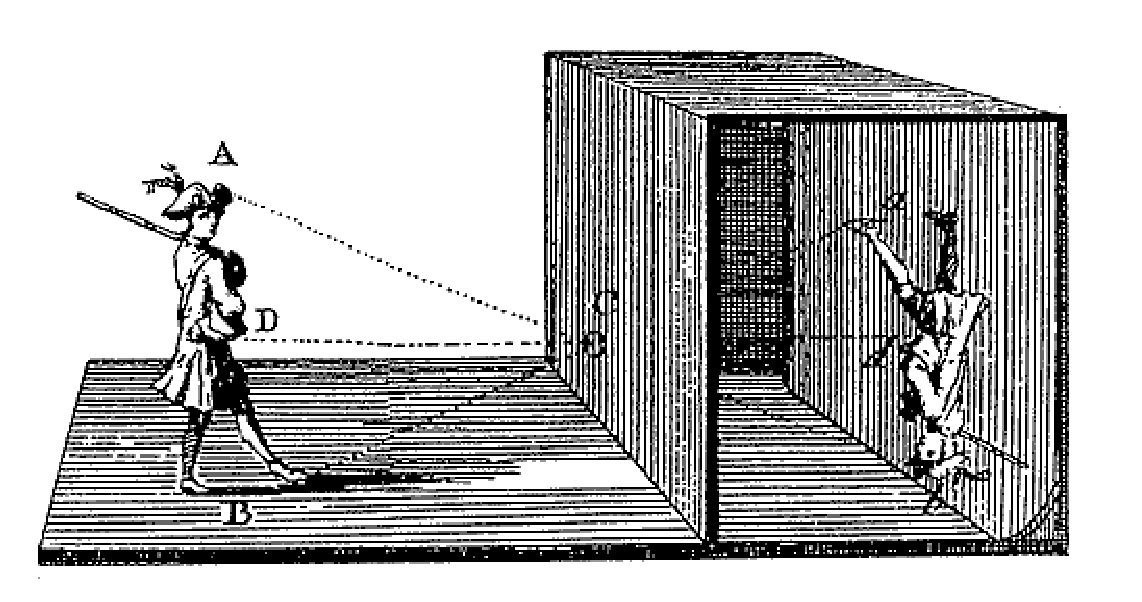
\includegraphics[width=12cm]{./pictures/cameraObscura}
	\caption[Athanasius Kircher, Principio della prospettiva nella camera obscura, 1671]{Athanasius Kircher, Principio della prospettiva nella camera obscura, 1671}
	\label{fig:prospettiva}
\end{figure} 
All'epoca di Brunelleschi, il modello del centro ottico veniva realizzato da una \textit{camera oscura}, come si pu\`o osservare nell'illustrazione in Figura \ref{fig:prospettiva}, mentre nei moderni sistemi di acquisizione viene realizzato tramite \textit{lenti ottiche}. 
\subsection{La matrice prospettica della camera}
\begin{figure}[tb]
	\centering
	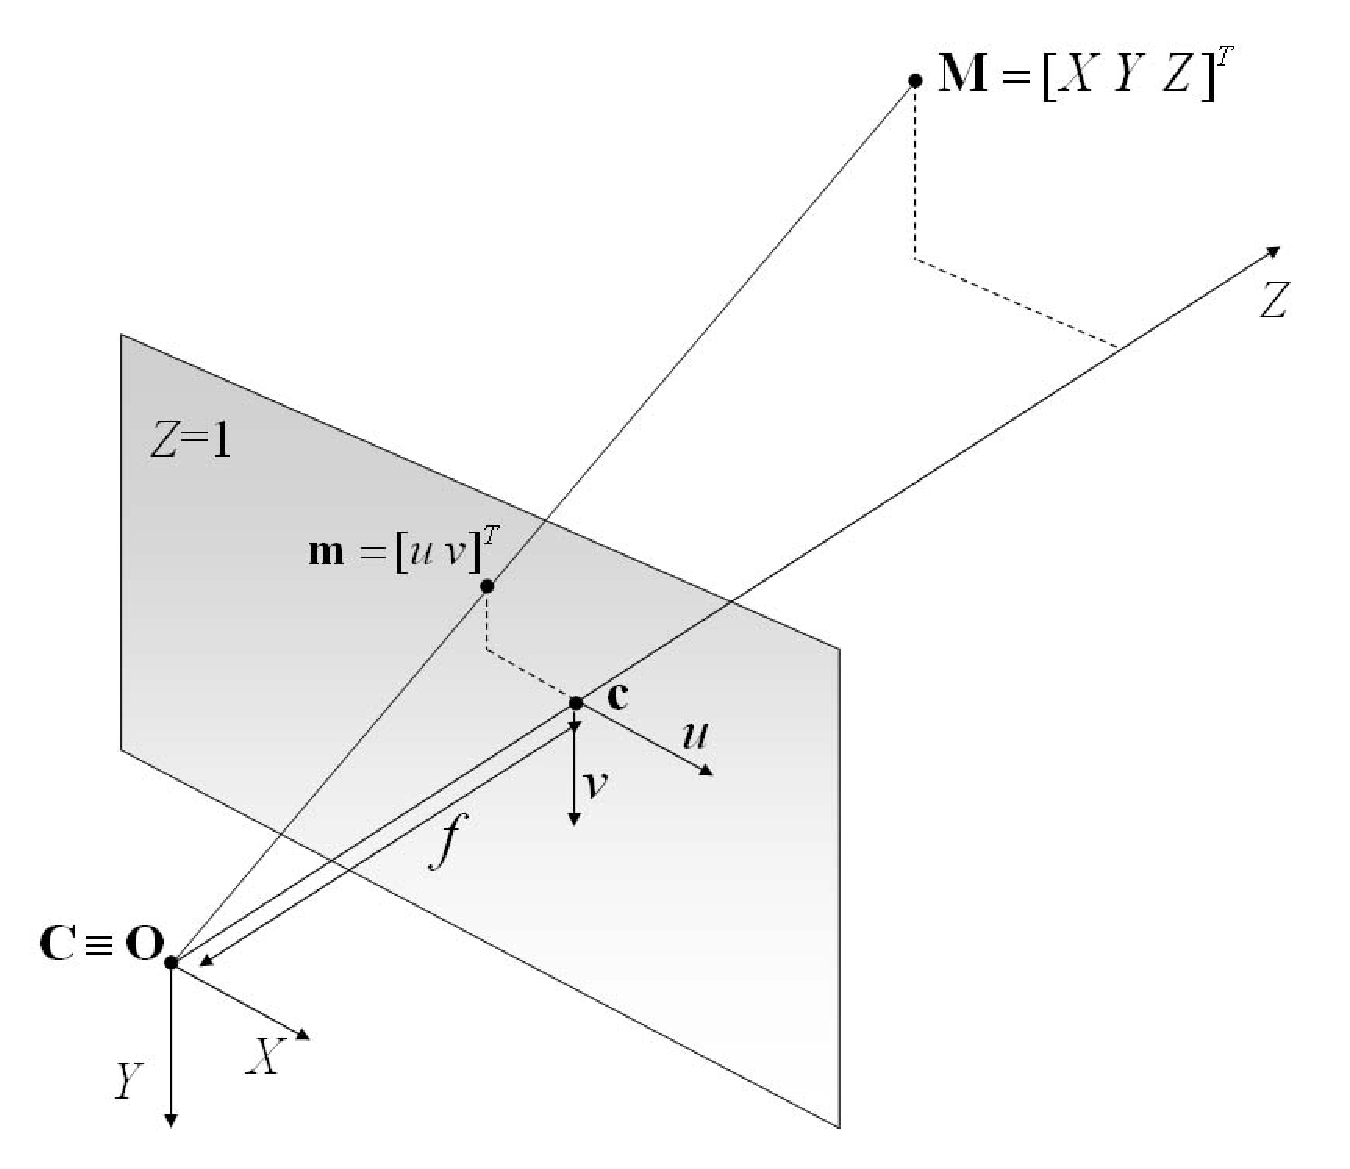
\includegraphics[width=10cm]{./pictures/modelloCamera}
	\caption{Schematizzazione del sistema ottico della camera}
	\label{fig:modelloCamera}
\end{figure} 
Nella Figura \ref{fig:modelloCamera} sono illustrati i concetti che sono utilizzati per descrivere il sistema ottico della camera.
Indichiamo con la lettera maiuscola $\textbf{M}=[X, Y, Z]^\textit{T}$ un qualsiasi punto nello spazio tridimensionale e con la lettera minuscola $\textbf{m} = [u, v]^\textit{T}$ la sua proiezione sul piano immagine dovuta al centro ottico $\textbf{C}$.
La linea che congiunge il centro ottico $\textbf{C}$ perpendicolarmente al piano immagine \`e detta \textit{asse principale}, indicata con $Z$, e il suo punto di intersezione con il piano stesso viene definita \textit{punto principale} $\textbf{c}$.
La distanza tra il punto principale e il centro ottico viene definita \textit{distanza focale},  e viene indicata con $f$.\\
La rappresentazione dei punti viene fatto attraverso le loro \textit{coordinate omogenee}.
In questo modo \`e possibile rappresentare le trasformazioni tra sistemi di coordinate di ordine differente tramite una singola trasformazione matriciale.
Chiamiamo coordinate omogenee di un punto $\textbf{m} = [u,v]$ del piano una qualsiasi terna ordinata $[U,V,W]$ di numeri reali tali che
\[W\neq 0,
\frac{U}{W}=u,
\frac{V}{W}=v.\]
Analogamente, le coordinate omogenee di un punto $\textbf{M}=[x,y,z]$ nello spazio tridimensionale saranno costituite da una quaterna di numeri $[X,Y,Z,W]$ tali che 
\[W\neq 0,
\frac{X}{W}=x,
\frac{Y}{W}=y,
\frac{Z}{W}=z.\]
La coordinata $W$ viene definita \textit{valore di scala}; nel caso $W=1$ le rimanenti coordinate omogenee rappresentano le \textit{coordinate cartesiane} del punto.\\
Consideriamo un punto $\textbf{M}$ nello spazio tridimensionale, rappresentato tramite le coordinate omogenee $[X,Y,Z,1]^\textit{T}$, e il suo punto immagine $\textbf{m}$ rappresentato dalle coordinate omogenee $[u,v,1]^\textit{T}$.
La proiezione della camera pu\`o essere espressa come
\begin{equation}
\label{eq:proiezione}
\textbf{m}=P\textbf{M},
\end{equation}
dove $P$ \`e una matrice di dimensioni $3 \times 4$ chiamata \textit{matrice prospettica} \cite{hartley2003multiple}.
Tale matrice contiene al suo interno informazioni sui parametri della camera a cui \`e associata, e descrive sia la proiezione sul piano immagine che le trasformazioni di camera rispetto al sistema di riferimento tridimensionale.
Formalmente la matrice prospettica viene definita attraverso la concatenazione di due matrici: una che rappresenta i \textit{parametri intrinseci} e un'altra che rappresenta i \textit{parametri estrinseci} \cite{forsyth2002computer}.
\begin{itemize}
	\item I \textit{parametri intrinseci} rappresentano le caratteristiche interne della camera come la distanza focale, il centro focale e le caratteristiche di \textit{distorsione} della lente.
	\item I \textit{parametri estrinseci} rappresentano la posizione della camera rispetto al sistema di riferimento dello spazio tridimensionale.
\end{itemize} 
\subsection{Parametri intrinseci}
\label{intrinsicParam}
La relazione fra le coordinate tridimensionali di un punto $\textbf{M}=[X,Y,Z]$ e le coordinate della sua proiezione $\textbf{m}=[u,v]$ \`e:
\[u=f\cdot \frac{X}{Z},\]
\[v=f\cdot \frac{Y}{Z}.\]
\begin{figure}[tb]
	\centering
	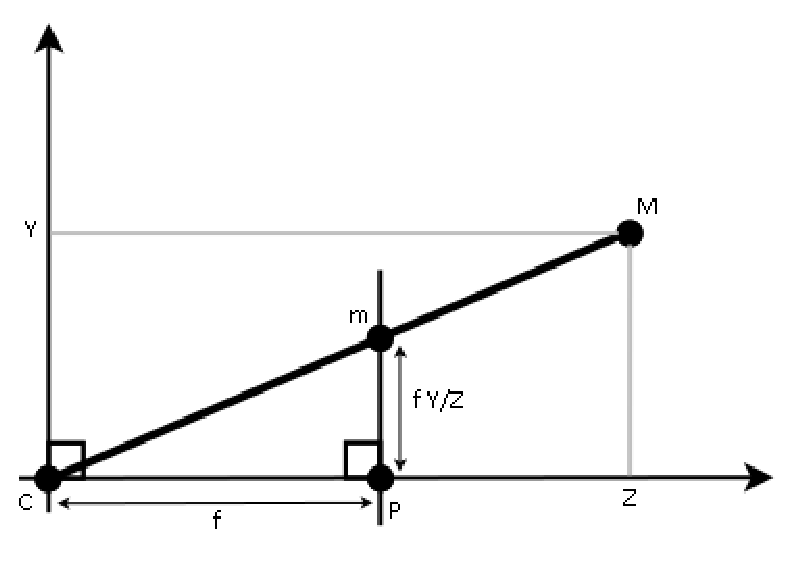
\includegraphics[width=10cm]{./pictures/mappatura2d3d}
	\caption{Similitudini tra triangoli usate nel calcolo dei parametri intrinseci}
	\label{fig:mapping}
\end{figure}
\noindent Tale relazione deriva dalle propriet\`a dei triangoli simili, come mostra la Figura \ref{fig:mapping}.
La \textit{mappatura} viene definita, dunque, dalla seguente relazione:
\begin{equation}
\label{eq:mapping}
[X,Y,Z]^\textit{T} \mapsto \left[f\cdot \frac{X}{Z}, f\cdot \frac{Y}{Z}\right]^\textit{T}.
\end{equation} 
Se il punto nello spazio e la sua proiezione sono rappresentati attraverso le loro coordinate omogenee, la \eqref{eq:mapping} pu\`o essere riscritta come
\begin{equation}
\label{eq:mappingMatrix}
\left[\begin{array}{c}
X \\ Y \\ Z \\ 1
\end{array}\right] \mapsto 
\left[\begin{array}{c}
f \cdot X \\ f \cdot Y \\ Z
\end{array}\right] = 
K \left[\begin{array}{rcl}
I & | & 0
\end{array}\right]
\left[\begin{array}{c}
X \\ Y \\ Z \\ 1
\end{array}\right],
\end{equation}
dove la matrice
\begin{equation}
\label{eq:kSimple}
K = 
\left[\begin{array}{rccl}
f & & \\
& f & \\
& & 1 
\end{array}\right]
\end{equation}

viene detta \textit{matrice di calibrazione} della camera.\\
Nella formula \eqref{eq:mapping} abbiamo assunto che l'origine delle coordinate del piano immagine si trovi nel punto principale, come \`e illustrato nella Figura \ref{fig:modelloCamera}.
Se consideriamo il punto principale di coordinate $[p_u, p_v]$, la \eqref{eq:mapping} diventa
 \begin{equation}
 \label{eq:mappingGeneral}
 [X,Y,Z]^\textit{T} \mapsto \left[f\cdot \frac{X}{Z}+p_u, f\cdot \frac{Y}{Z}+p_v\right]^\textit{T},
 \end{equation}
 mentre la matrice di calibrazione\eqref{eq:kSimple} diventa 
 \begin{equation}
 \label{eq:kGeneral}
 K =
  \left[\begin{array}{rcl}
  f & & p_u \\
  & f & p_v \\
  & & 1 
  \end{array}\right].
 \end{equation}
 Nel caso in cui il sensore della camera sia \textit{digitale}, l'immagine deve essere quantizzata come una matrice di $W$ colonne e $H$ righe, in cui ciascun elemento prende il nome di \textit{pixel} (dalla contrazione di \textit{picture element}).
 \begin{figure}[tb]
 	\centering
 	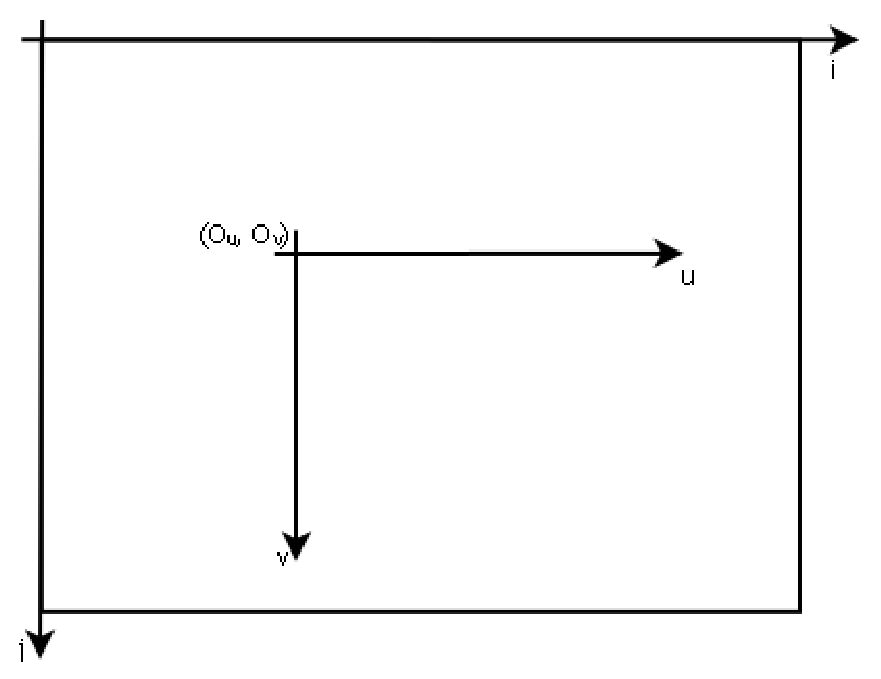
\includegraphics[width=8cm]{./pictures/griglia}
 	\caption{Coordinate di un frame}
 	\label{fig:griglia}
 \end{figure}
 Ogni pixel possiede, quindi, delle coordinate che definiscono la sua posizione sulla matrice del frame.
 Se definiamo con $(i,j)$ le coordinate del generico pixel sulla matrice del frame, dove l'origine \`e posta nell'angolo in alto a sinistra, e con $(O_u, O_v)$ le coordinate del punto principale secondo il sistema di riferimento del frame (si veda a riguardo la Figura \ref{fig:griglia}), possiamo mettere in relazione le coordinate dell'immagine con le coordinate frame nel seguente modo:
 \[ u = (i - O_u) \cdot S_u \]
 e
 \[ v = (j - O_v) \cdot S_v, \]
 dove $S_u$ e $S_v$ sono le dimensioni orizzontali e verticali del singolo pixel.
 \`E necessario introdurre, nella matrice di calibrazione, l'informazione del numero di pixel per unit\`a di distanza in coordinate immagine $m_u$ e $m_v$, rispettivamente nelle direzioni $u$ e $v$, modificando la matrice di calibrazione definita in \eqref{eq:kGeneral} come
 \begin{equation}
 \label{eq:kDigital}
 K =
 \left[\begin{array}{rccl}
 \alpha_u & & u_0\\
 & \alpha_v & v_0\\
 & & 1
 \end{array}\right],
 \end{equation}
 dove $\alpha_u = fm_u$ e $\alpha_v=fm_v$, mentre il punto principale $[p_u, p_v]$ viene riscritto come $[u_0, v_0] = [m_u p_u, m_v p_v]$. \\
 Nel caso in cui la matrice di calibrazione sia nota, la camera viene detta \textit{completamente calibrata}.\\
 La matrice di calibrazione $K$ rappresenta, quindi, il cambio di sistema di riferimento nel piano immagine, ridefinendo il centro della camera $(u_0, v_0)$ in modo che coincida con il punto principale.
 \subsection{Parametri estrinseci}
 La matrice $K$ descritta dall'equazione \eqref{eq:kDigital} \`e valida per camere poste all'origine del sistema di riferimento.
Se consideriamo delle camere poste in un punto arbitrario dell'ambiente, quindi, \`e necessario che le coordinate dei punti, definite nel sistema di riferimento tridimensionale, siano ridefinite secondo il sistema di coordinate della camera.
 \begin{figure}[tb]
 	\centering
 	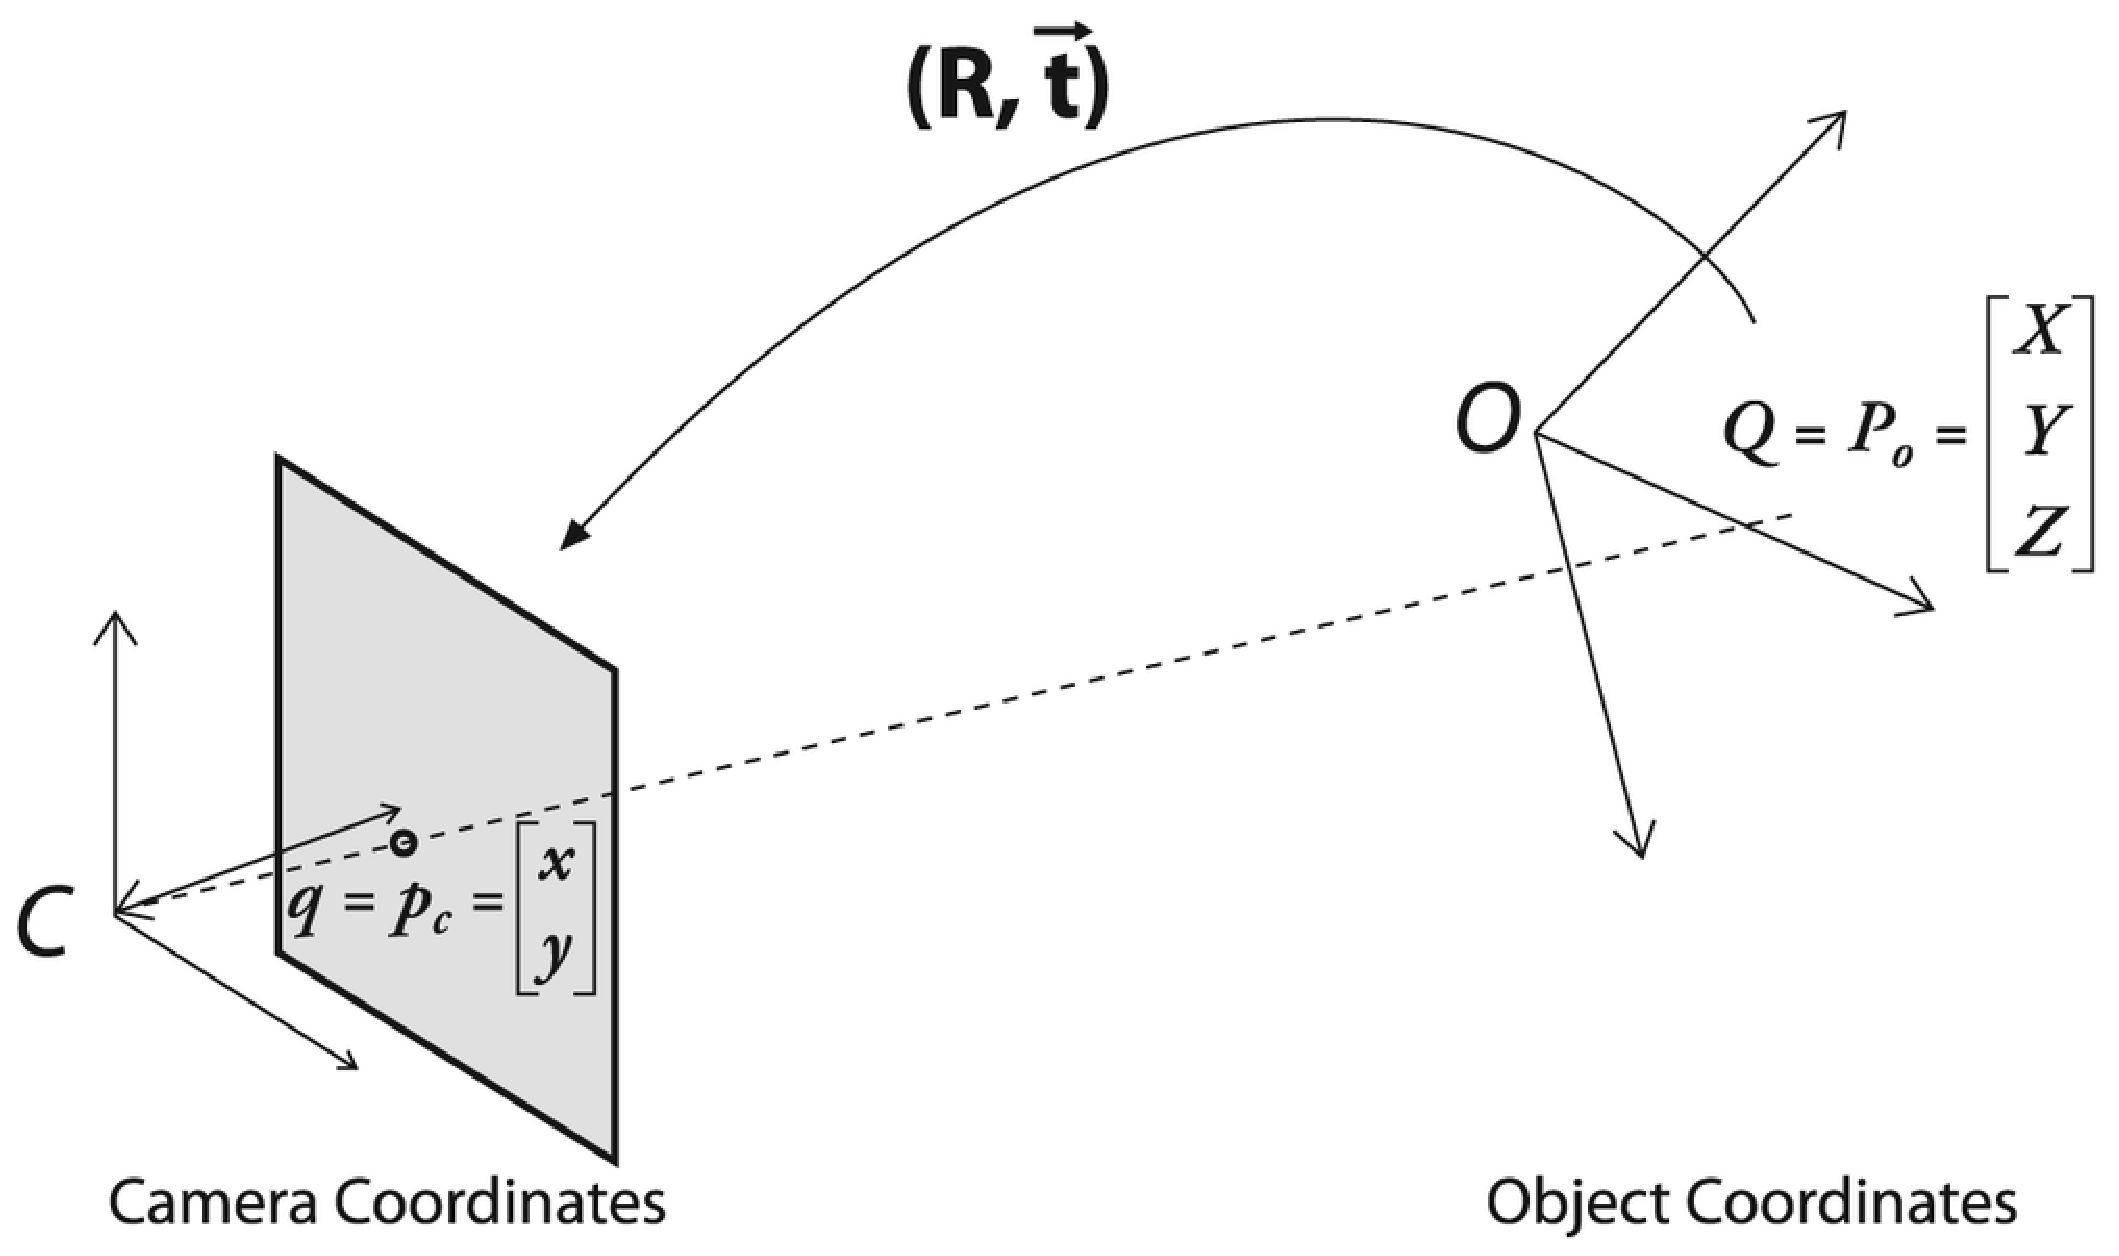
\includegraphics[width=8cm]{./pictures/rt}
 	\caption{Trasformazione dal sistema di coordinate dell'ambiente a quello della camera}
 	\label{fig:rt}
 \end{figure}
Questa trasformazione viene definita attraverso una \textit{rototraslazione}, nello spazio, del sistema di riferimento dell'ambiente, in modo che coincida con quello della camera.
Se $\tilde{\textbf{M}}$ rappresenta le coordinate cartesiane di un punto nel sistema di riferimento dell'ambiente e $\tilde{\textbf{M}}_{cam}$ rappresenta lo stesso punto nel sistema di riferimento della camera, si pu\`o scrivere
\begin{equation}
\label{eq:rototrals1}
\tilde{\textbf{M}}_{cam}=R(\tilde{\textbf{M}} - C),
\end{equation}
dove $C$ rappresenta le coordinate del centro della camera nel sistema di riferimento dell'ambiente, $R$ \`e una \textit{matrice di rotazione} $3 \times 3$ che rappresenta l'orientamento della camera rispetto al sistema di riferimento dell'ambiente e $K$ \`e la matrice di calibrazione della camera.
L'equazione \eqref{eq:rototrals1} pu\`o essere riscritta in forma matriciale: se definiamo $\textbf{M}$ e $\textbf{M}_{cam}$ come le rappresentazioni in coordinate omogenee di $\tilde{\textbf{M}}$ e $\tilde{\textbf{M}}_{cam}$, abbiamo
\[ \textbf{M}_{cam} =  \left[\begin{array}{cc}
R & -RC \\
0 & 1
\end{array}\right] 
\textbf{M}, \]
da cui, riprendendo l'equazione \ref{eq:mappingMatrix},
\begin{eqnarray}
\textbf{m} & = & K \left[\begin{array}{rcl}
I & | & 0
\end{array}\right]\textbf{M}_{cam} \nonumber \\
 & = & K \left[\begin{array}{rcl}
I & | & 0
\end{array}\right] 
\left[\begin{array}{cc}
R & -RC\\
0 & 1 
\end{array}\right] \textbf{M} \nonumber \\
 & = &
K \left[\begin{array}{rcl}
R & | & -RC
\end{array}\right]\textbf{M}. \nonumber
\end{eqnarray}
Possiamo, quindi, scrivere l'equazione della matrice di proiezione della camera come
\[P=K \left[\begin{array}{rcl}
R & | & t
\end{array}\right],\]
dove $t = -RC$ prende il nome di \textit{vettore di traslazione}.
%\section{Monitoraggio video: concetti e terminologia}
%Prima di concentrarci sul problema del tampering detection, definiamo, i concetti e i termini che verranno utilizzati nel seguito della trattazione.\\
%Lo scenario che consideriamo \`e quello di una camera che deve riprendere una particolare \textit{\gls{scena}}.
%\begin{figure}
%	\centering
%	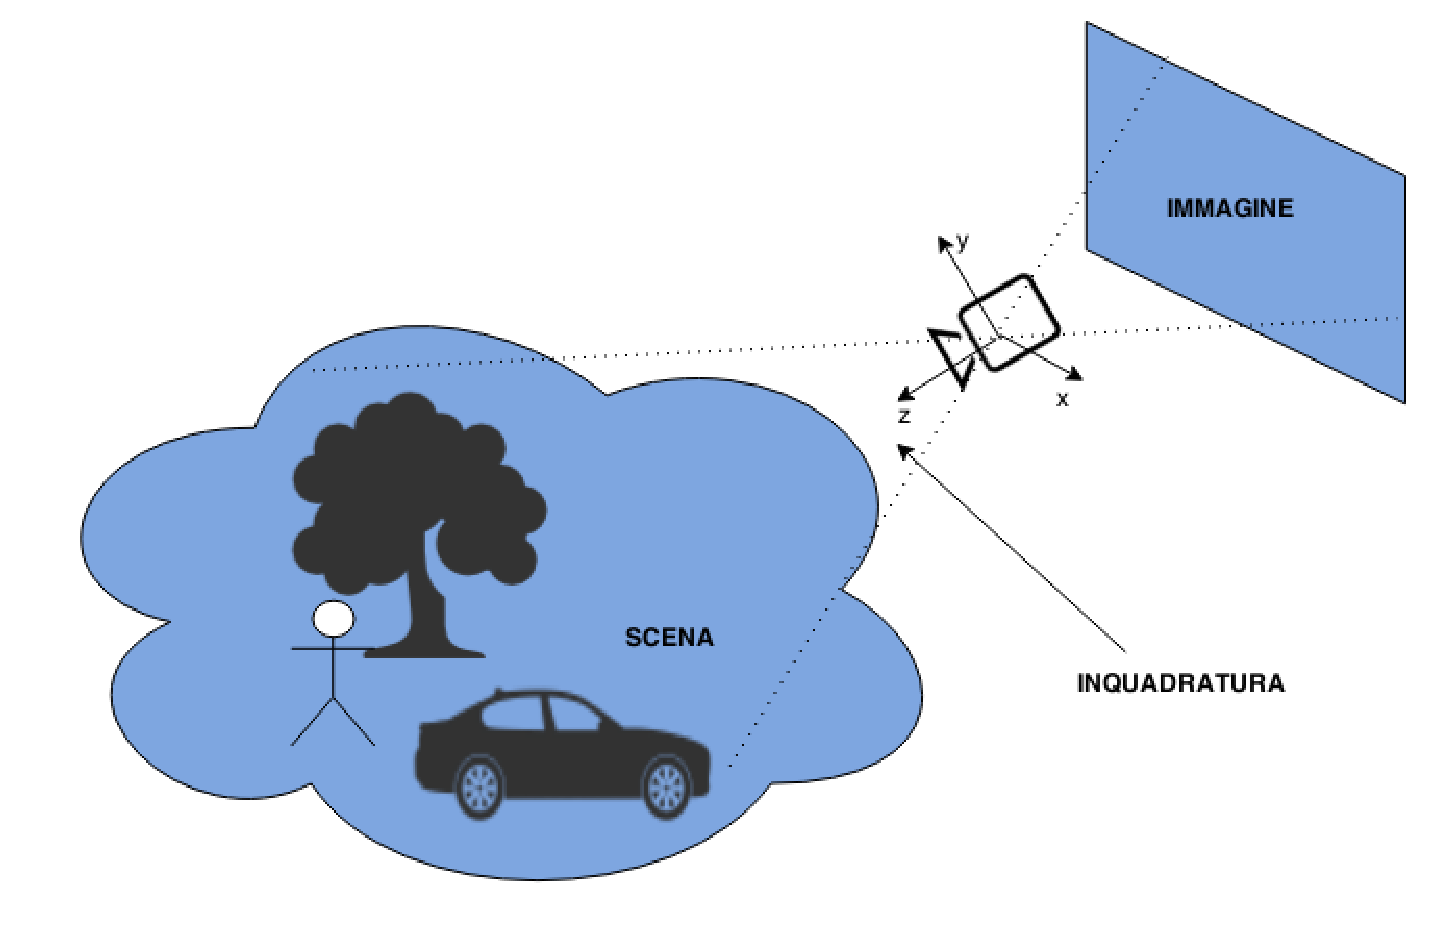
\includegraphics[width=12cm]{./pictures/videoMonitoring}
%	\caption{Sistema di monitoraggio video}
%	\label{fig:videoMonitoring}
%\end{figure}
%\noindent 
%La posizione e l'orientamento della camera determinano l'\textit{\gls{inquadratura}} della scena.
%L'acquisizione, da parte della camera, della scena nell'istante di tempo $i$ viene definita \textit{immagine} o \textit{frame} i-esimo.
%La Figura \ref{fig:videoMonitoring} illustra questi concetti.\\
%Per semplificare l'analisi, considereremo immagini estratte in \textit{scala di grigi}.
%Quindi ciascuna immagine verr\`a rappresentata come una matrice di pixel, in cui ciascun elemento rappresenta l'intensit\`a luminosa (\textit{luma}) del pixel corrispondente.\\
%Nel seguito della trattazione useremo una specifica terminologia.
%Indicheremo con $\mathcal{X}$ l'insieme dei \textit{pixel} costituenti l'immagine acquisita dalla camera,
%\[ \mathcal{X} \subset \mathbb{N}^2, \]
%e con $x \in \mathcal{X}$ il singolo pixel.
%Quando vorremo considerare il frame acquisito all'istante di tempo $i$, useremo $z_i$, con $i=1,\dots , \infty$. 
%In particolare, per indicare il valore della \textit{luminosit\`a} del pixel $x$ per il frame $i$-esimo, useremo il termine $z_i(x)$, con 
%\[ z_i(x) \in [0, 255]. \]
\section{Rappresentazione digitale delle immagini}
\label{rappresentazImmagini}
Nel Paragrafo \ref{intrinsicParam} abbiamo introdotto il concetto di \textit{immagine digitale} come rappresentazione numerica dell'immagine bidimensionale.
	\begin{figure}[tb]
		\centering
		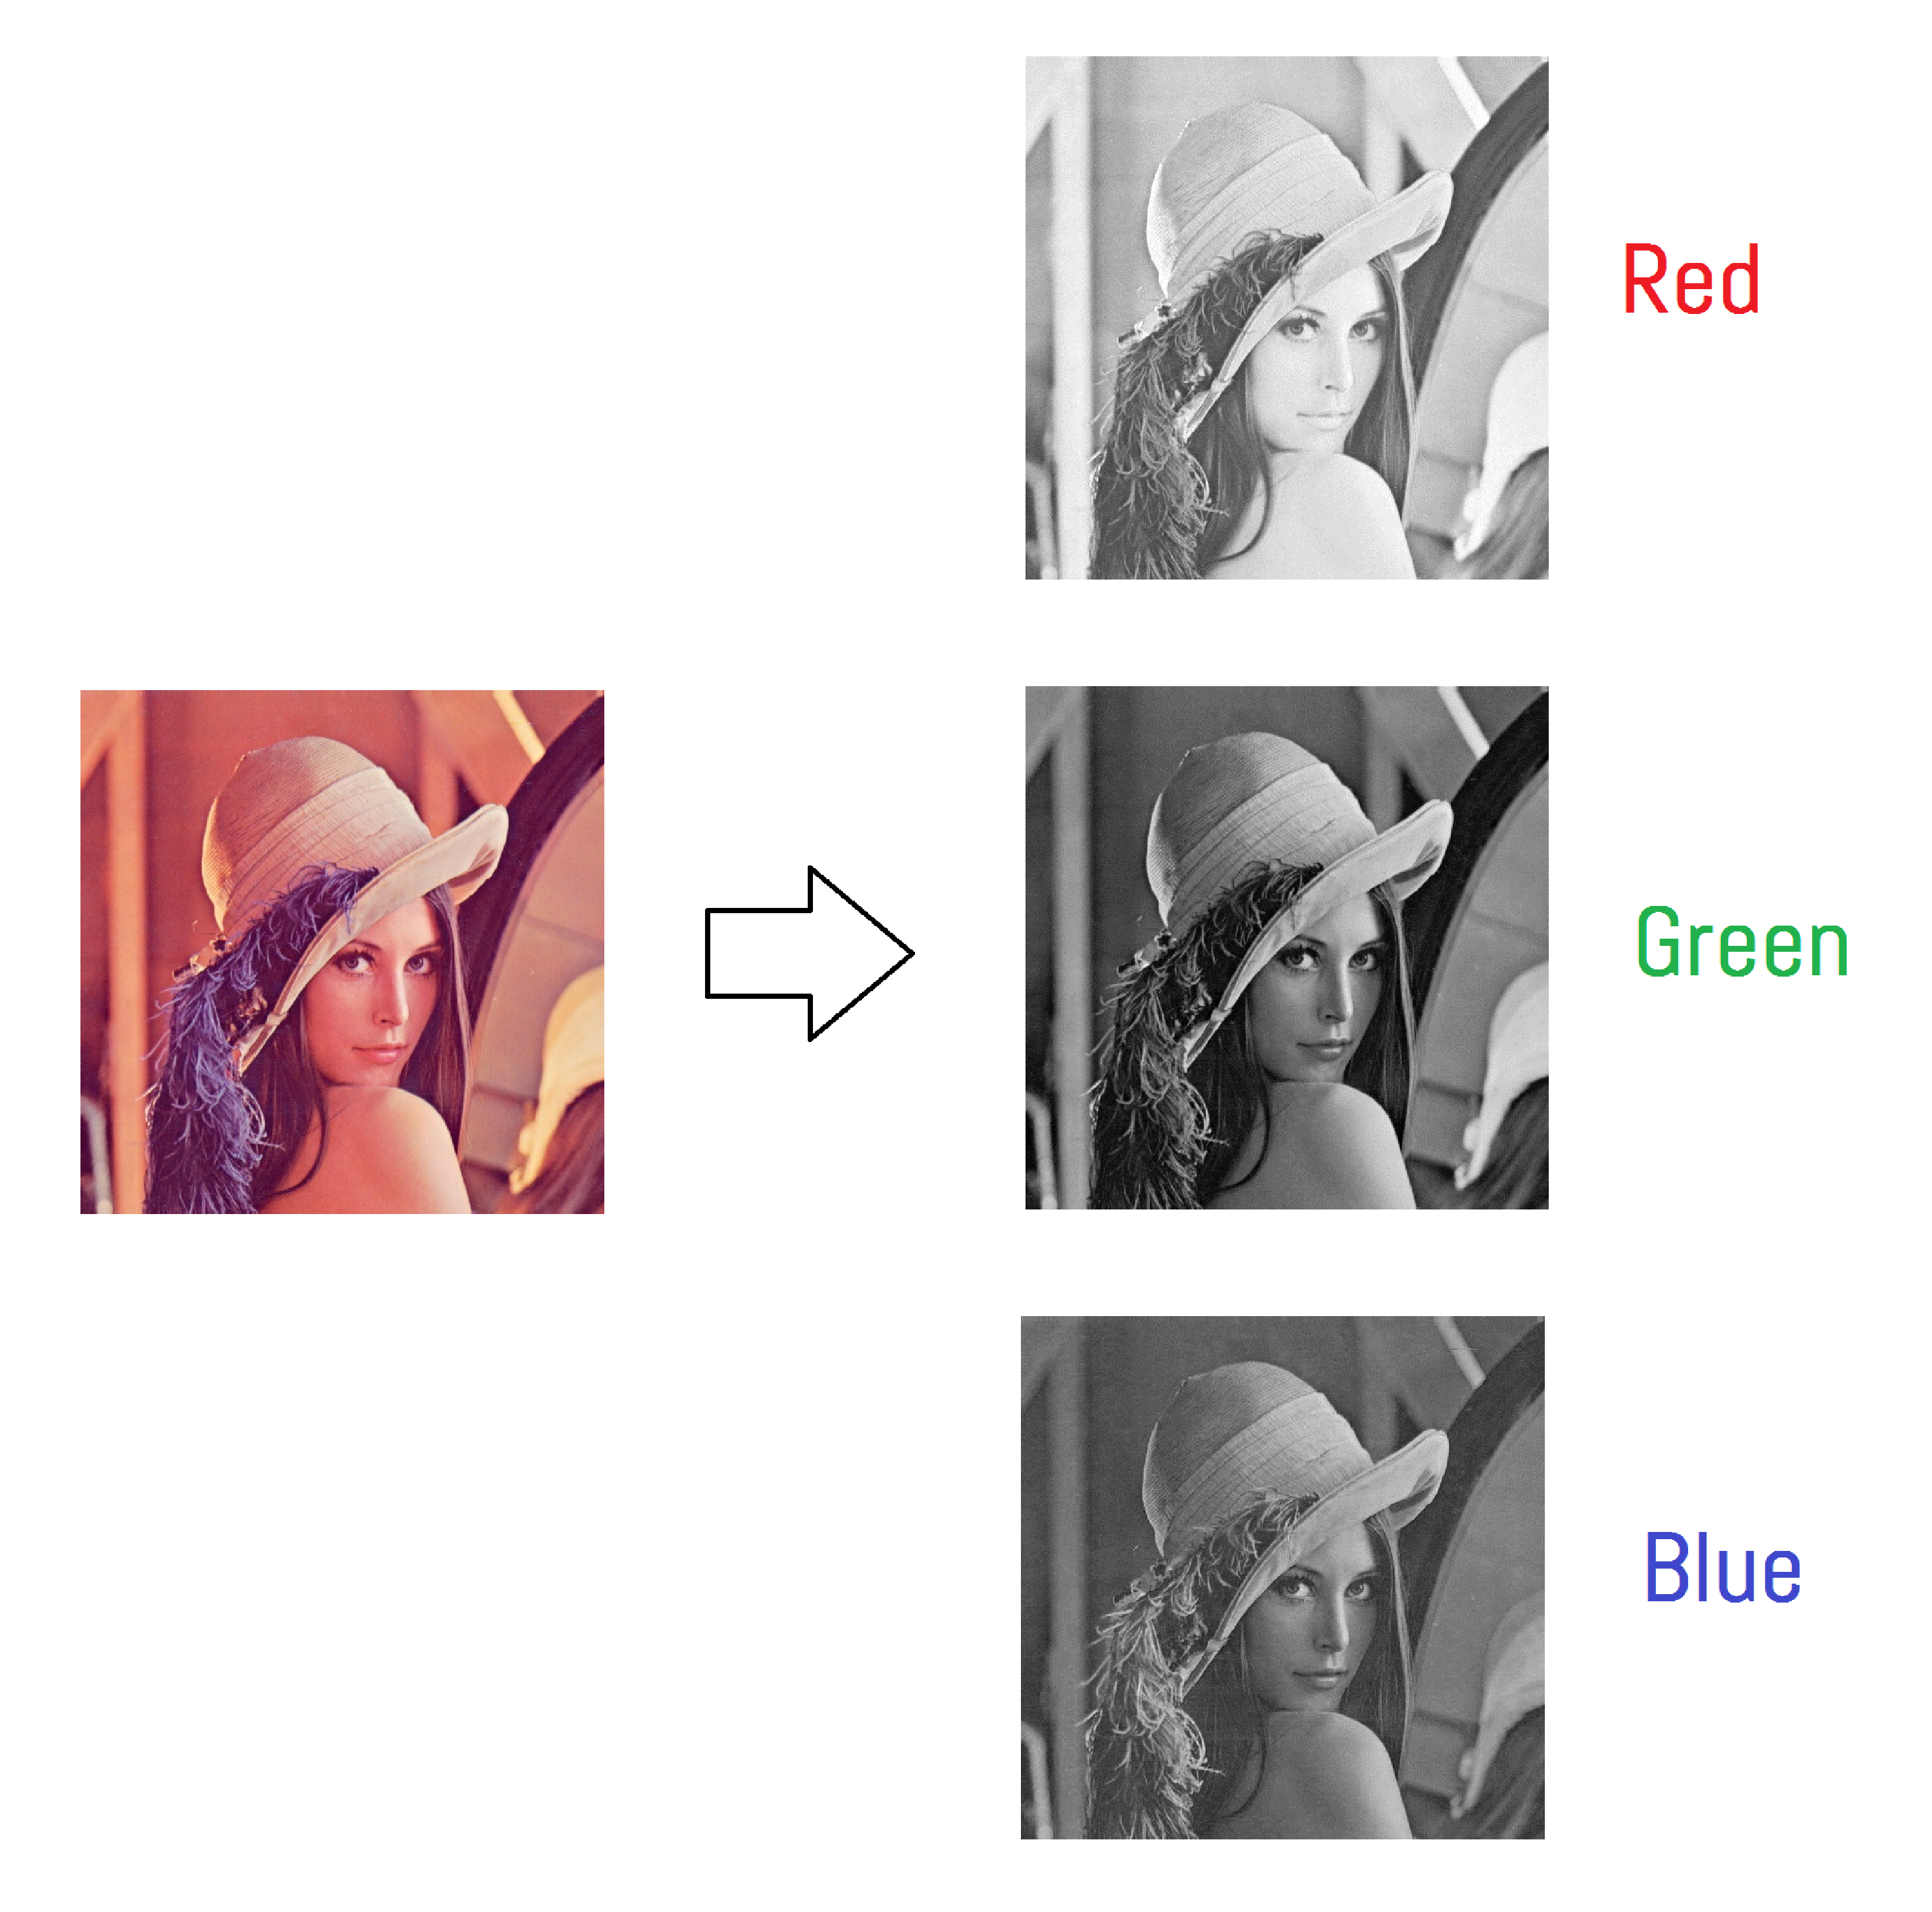
\includegraphics[width=8cm]{./pictures/lenaRGB}
		\caption{Esempio di estrazione dei canali RGB}
		\label{fig:lenaRGB}
	\end{figure}
Esistono vari modi di rappresentare un'immagine in formato digitale.
Le rappresentazioni che a noi interessa considerare sono \cite{forsyth2002computer}:
\begin{itemize}
	\item \textit{scala di grigi}, in cui l'immagine \`e rappresentata come una matrice $\textbf{I}$ di dimensioni $H \times W$, dove l'elemento $\textbf{I}(i,j)$ rappresenta il valore di \textit{intensit\`a luminosa} (\textit{luma}) del pixel di coordinate $(i, j)$;
	\item \textit{RGB}, dove l'immagine \`e rappresentata come una matrice \textit{tridimensionale} $\textbf{I}_{RGB}$ di dimensioni $H \times W \times 3$, in cui vengono memorizzati i livelli di intensit\`a luminosa dei tre colori fondamentali \textit{rosso} (R), \textit{verde} (G) e \textit{blu} (B) per ciascun pixel (Figura \ref{fig:lenaRGB}); 
	\item \textit{YUV}, in cui lo spazio colore viene definito tramite un componente di luma (Y) e due componenti di \textit{crominanza} (UV), che rappresentano rispettivamente i valori di differenza dal colore blu ($U = B - Y$) e dal colore rosso ($V = R - Y$) (Figura \ref{fig:yuv}).
\end{itemize}
Le immagini digitali possono essere memorizzate in diversi formati.
Spesso vengono utilizzati algoritmi di \textit{compressione}, che possono essere
\begin{itemize}
	\item a perdita di informazione (\textit{lossy}), come nel caso delle immagini \textit{JPEG};
	\item senza perdita di informazione (\textit{lossless}), come nel caso dei file d'immagine \textit{PNG} o \textit{GIF}.
\end{itemize}
	\begin{figure}[tb]
		\centering
		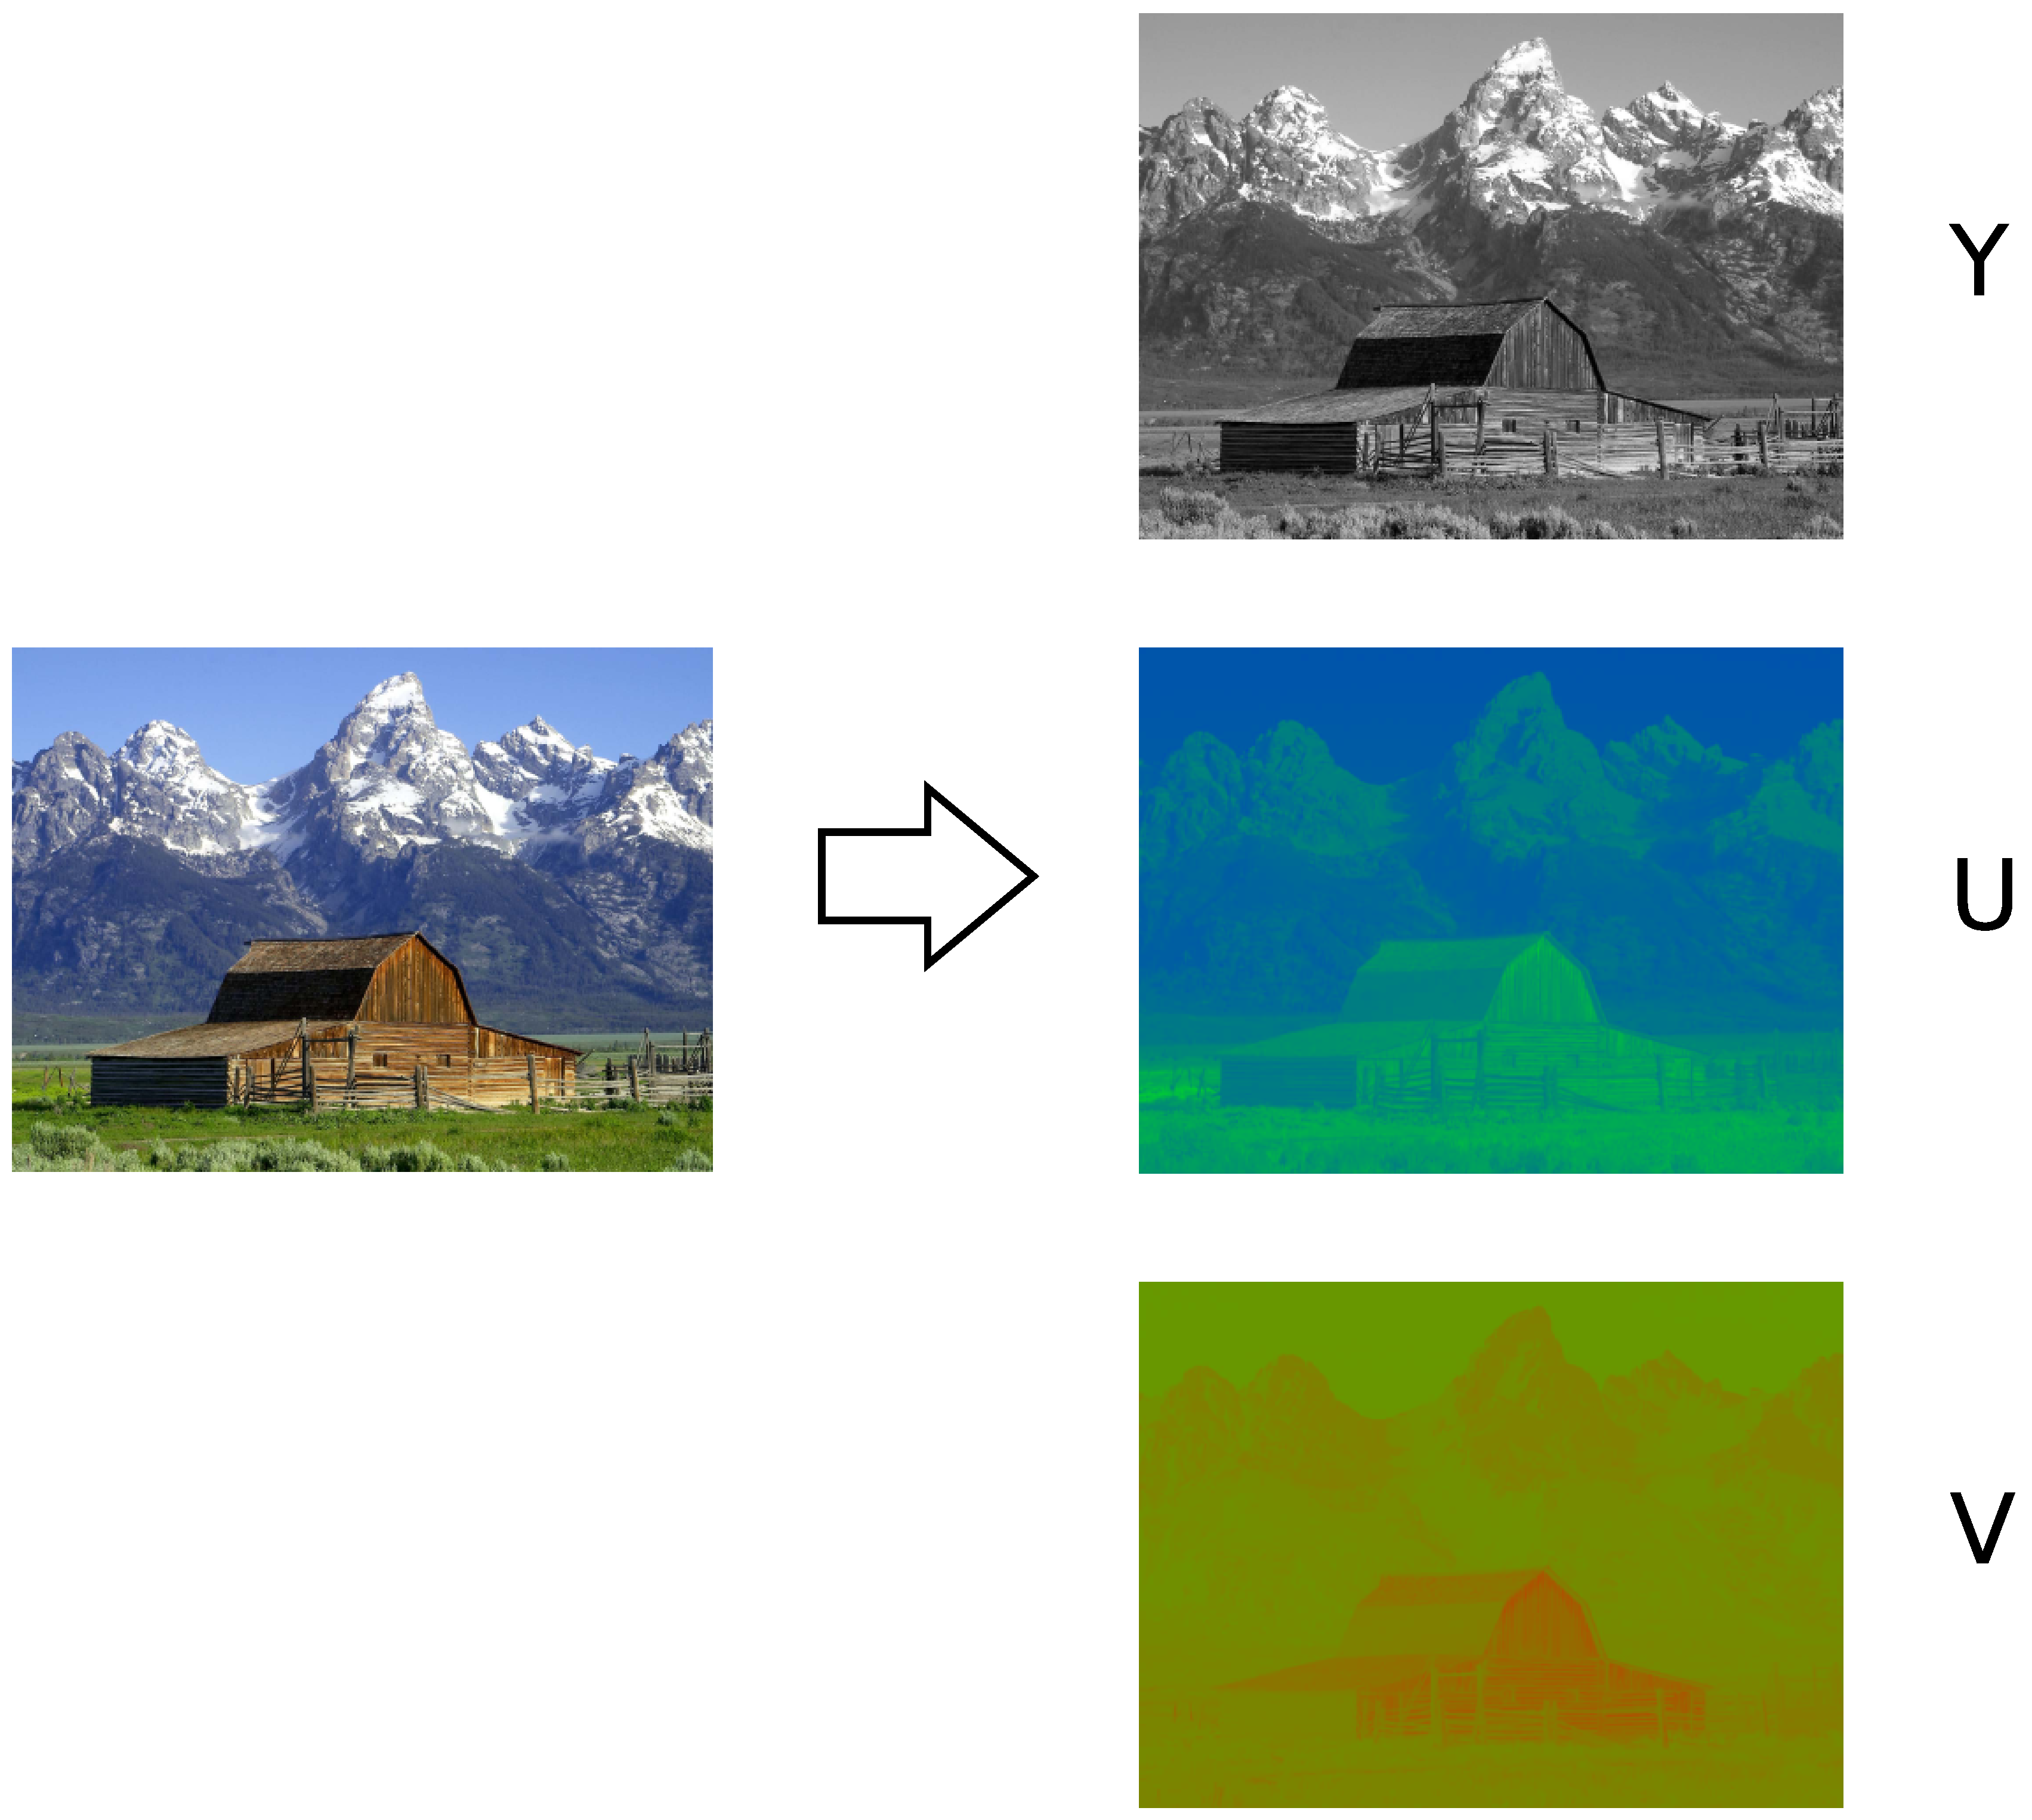
\includegraphics[width=8cm]{./pictures/yuv}
		\caption{Esempio di estrazione dei canali YUV}
		\label{fig:yuv}
	\end{figure}
	



\section{Identificazione del cambiamento nella stazionariet\`a di un processo}
\label{cdt}
Prima di illustrare come \`e stato affrontato il problema del tampering detection nella letteratura scientifica, affrontiamo il problema, pi\`u generale, di come identificare un cambiamento all'interno di un processo.
Una caratteristica, richiesta in molte applicazioni di analisi e elaborazione intelligente di dati, riguarda l'assunzione che il processo generante questi dati non cambi nel tempo \cite{alippi2014intelligence}. In questo caso si parla di processi \textit{stazionari}, ovvero processi dove i dati possono essere considerati generati da un'unica distribuzione probabilistica. \\
In molte situazioni, soprattutto se vengono utilizzati dei sensori per misurare delle grandezze fisiche, si pu\`o incorrere in situazioni in cui questa ipotesi di stazionariet\`a venga meno.
Ad esempio, pu\`o succedere che il sensore si guasti, oppure che fenomeni esterni non permettano un'acquisizione ottimale. 
In questi casi \`e opportuno avere a disposizione degli strumenti in grado di identificare quando la condizione di stazionariet\`a di un processo viene meno, in modo da poter lanciare un allarme a riguardo. 
Le tecniche principalmente utilizzate per questo scopo prendono il nome di \textit{Change-Point Methods} (CPM) e \textit{Change-Detection Tests} (CDT), e verranno illustrate nel resto del paragrafo.	
\subsection{Metodi di Change-Point}
I metodi di Change-Point (CPM) vengono utilizzati per ispezionare una certa sequenza di dati e verificare la sua stazionariet\`a. 
Ci\`o viene fatto verificando che, all'interno della sequenza, esista un istante temporale in cui la distribuzione dei dati cambia (\textit{change point}).\\
In maniera formale possiamo dire che, data una sequenza di dati
\[\mathcal{X}=\{x(t), t = 1,...,n\},\]
essa contiene un change point all'istante $\tau < n$ se \`e possibile
suddividerla in due sotto-sequenze
\[ \begin{array}{l}
\mathcal{A}_\tau = \{x(t), t = 1,...,\tau \}\\
 \mathcal{B}_\tau = \{x(t), t = \tau + 1,...,n \}
\end{array},\]
le quali sono due realizzazioni \textit{indipendenti e identicamente distribuite} (i.i.d.) di due differenti variabili aleatorie con distribuzione $ \mathcal{F}_0 $ e $ \mathcal{F}_1 $.
\`E possibile, quindi,  convertire il problema del change point in uno equivalente dove si valuta se $ \mathcal{A}_\tau $ e $ \mathcal{B}_\tau $ sono generati da due distribuzioni diverse.\\
Il problema, a questo punto, pu\`o essere riformulato come un \textit{test d'ipotesi a due campioni} \cite{ross2009introduction}, dove l'\textit{ipotesi nulla} ($ H_0 $) e l'\textit{ipotesi alternativa} ($ H_1 $) sono le seguenti:
\[ \begin{array}{rcl}
H_0: &  x(t) \sim &  \mathcal{F}_0 \quad  \forall t \\
H_1: &  x(t) \sim &
\begin{cases}
\mathcal{F}_{0} & \text{se } t < \tau \\
\mathcal{F}_{1} & \text{se } t \geq \tau
\end{cases}
\end{array}. \]
Per la valutazione delle ipotesi fatte sopra, occorrono delle opportune \textit{statistiche di test a due campioni} 
\[ \mathcal{T}_\tau = \mathcal{T}(\mathcal{A}_\tau, \mathcal{B}_\tau), \]
in modo da poter comparare $ \mathcal{A}_\tau $ e $ \mathcal{B}_\tau $. In questo modo \`e possibile rifiutare l'ipotesi nulla quando il valore della statistica $ \mathcal{T}_\tau $ supera una certa soglia $ h_{n,\alpha} $, calcolata in funzione di un certo \textit{intervallo di confidenza} $ \alpha $ e del numero di campioni $ n $.\\
Se, ad esempio, consideriamo l'ipotesi che $
\mathcal{A}_\tau $
e $ \mathcal{B}_\tau $ siano generate da due
distribuzioni \textit{gaussiane}, \`e
possibile valutare la dissimilarit\`a tra le
due distribuzioni controllando i due
\textit{valori attesi}. Possiamo usare, come
statistica di test, la \textit{differenza
	standardizzata tra le medie di due
	campioni}, definita come
\[ D_\tau = \sqrt{\frac{\tau(n-\tau)}{n}}
\frac{\overline{\mathcal{A}}_\tau-\overline{\mathcal{B}}_\tau}{S_\tau}, \]
dove $ \overline{\mathcal{A}}_\tau $ e $ \overline{\mathcal{B}}_\tau $ denotano le \textit{medie campionarie} valutate rispettivamente su $ \mathcal{A}_\tau $ e $ \mathcal{B}_\tau $, mentre $ S_\tau $ \`e la \textit{varianza campionaria} valutata \textit{su tutto l'insieme dei dati}.\\
Quando la statistica di test utilizzata,
corrispondente a una specifica partizione
dell'insieme dei dati, non fornisce l'evidenza
necessaria a rifiutare $ H_0, $ l'unica cosa
che \`e possibile stabilire \`e che
nell'istante $ \tau $ scelto non si \`e avuto
un cambiamento nella stazionariet\`a
dell'insieme. \textit{Ci\`o non implica che	l'istante di cambiamento non sia un altro ancora da valutare.} 
In maniera rigorosa \`e necessario valutare, quindi, tutte le possibili partizioni dell'insieme dei dati considerati. 
Le ipotesi nulla e alternativa vengono, perci\`o, modificate nel seguente modo \cite{ross2011nonparametric}:
\[
\begin{array}{rccl}
H_0 :& \forall t, & x(t) \sim & \mathcal{F}_0 \\
H_1 :& \exists \tau & x(t) \sim &
\begin{cases}
\mathcal{F}_{0} & \text{se } t < \tau \\
\mathcal{F}_{1} & \text{se } t
\geq \tau
\end{cases}
\end{array}.
\]
Entrando pi\`u nel dettaglio, per ciascun
punto $ s \in \{2,...,n-1\} $, candidato a
essere un change point, valutiamo la
statistica di test $ \mathcal{T}_s. $ Viene scelto come
change point quello che massimizza la
statistica
\[ M= \argmax_{s=2,...,n-1} (\mathcal{T}_s), \]
corrispondente al valore $ \mathcal{T}_M $ di $\mathcal{T}$
\[ \mathcal{T}_M = \max_{s=2,...,n-1} (\mathcal{T}_s).\]
Una volta trovato $\mathcal{T}_M$ il test va finalizzato
comparando questa statistica con la soglia
$ h_{n,\alpha}, $ in modo da verificare se
l'ipotesi nulla sia da scartare o meno.
\begin{figure}
	\centering
	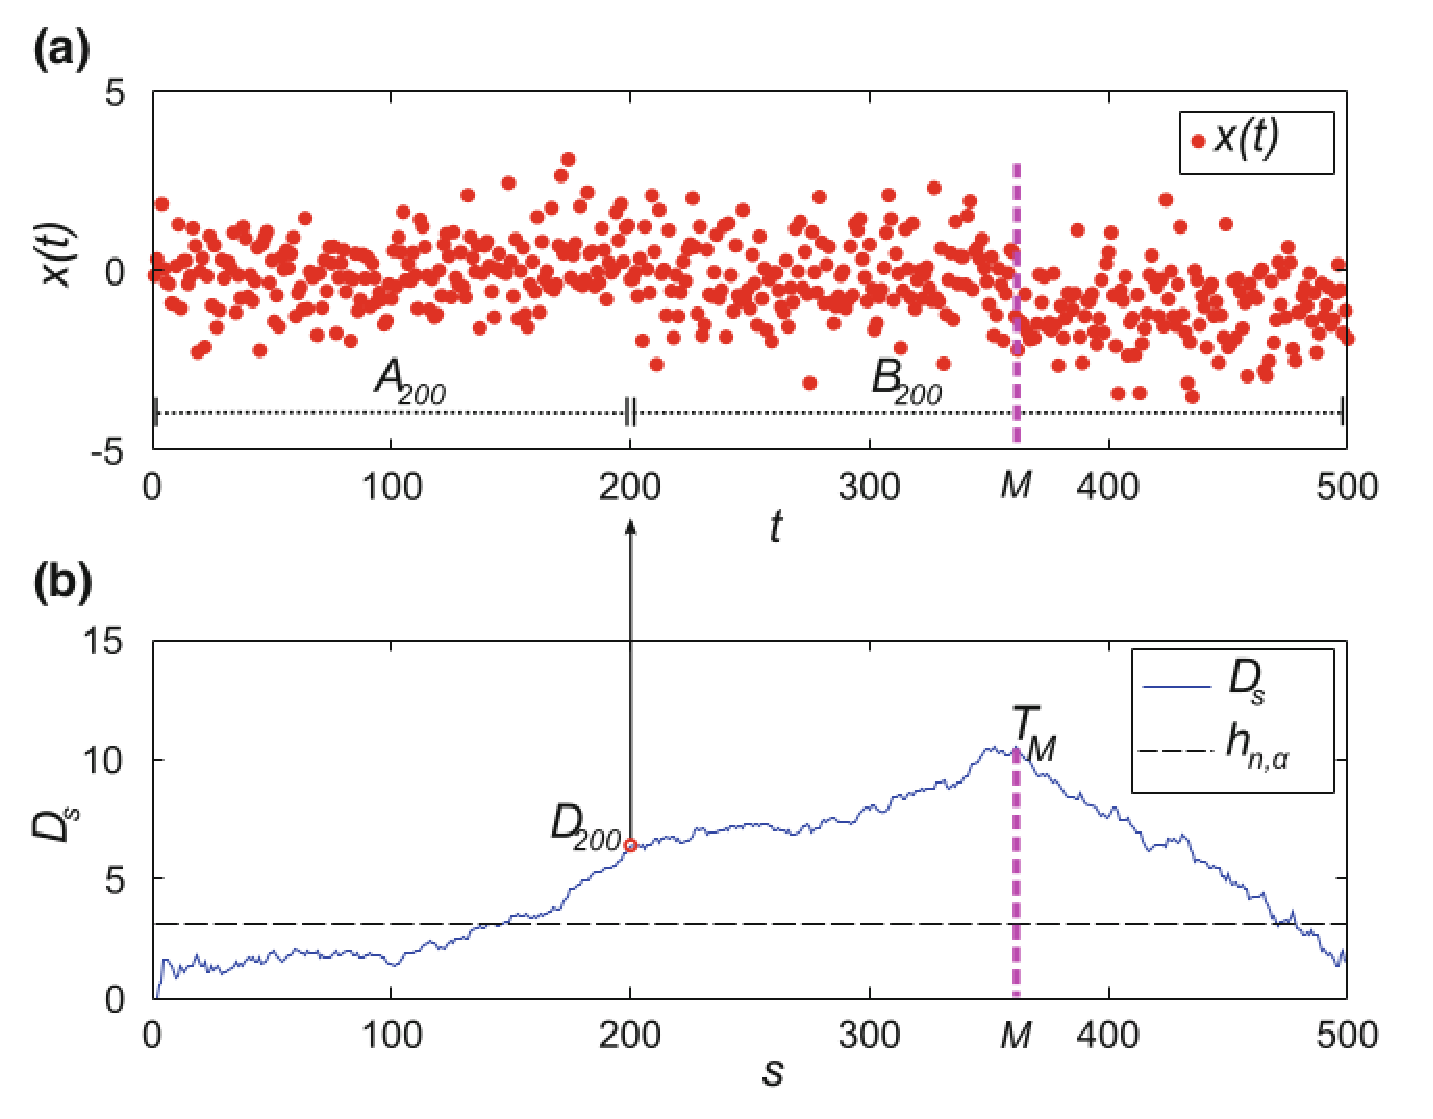
\includegraphics[width=12cm,keepaspectratio]{pictures/CPM}
	\caption{Esempio di CPM}
	\label{fig:CPM}
\end{figure}
Nella Figura \ref{fig:CPM} possiamo vedere un esempio di CPM basato su una statistica \textit{t di Student} \cite{alippi2014intelligence}. La sequenza \`e formata da 500 dati (\textbf{a}) ed \`e stato individuato un cambiamento all'istante $\tau=350$. I valori delle varie statistiche in funzione di s sono visualizzati in (\textbf{b}).\\
Spesso \`e preferibile utilizzare dei test
statistici \textit{non parametrici},
soprattutto quando le distribuzioni dei dati
sono incognite. Le statistiche maggiormente
utilizzate sono quelle basate su
\textit{calcolo del rango}
\cite{ross2011nonparametric}. Quando si ha a
che fare con cambiamenti nella
\textit{localit\`a} dei dati una statistica
solitamente utilizzata \`e quella di
\textit{Mann-Whitney}, mentre quando si
vogliono verificare cambiamenti \textit{di
	scala} \`e possibile utilizzare la
statistica di \textit{Mood}. La statistica di
\textit{Lepage} invece pu\`o risultare utile
per analizzare entrambi i tipi di
cambiamento. Un altro approccio consiste nel
comparare le \textit{distribuzioni empiriche}
dei due insiemi di dati, usando ad esempio la
statistica di \textit{Kolmogorov-Smirnov}.
\subsection{Change-Detection Test}
I metodi di change point sono stati principalmente
pensati per essere eseguiti \textit{a valle} della
completa acquisizione dei dati. Inoltre il suo elevato
costo computazionale fa s\`i che questa tecnica
difficilmente possa essere utilizzabile all'interno di
un sistema embedded. Le tecniche che vengono descritte
in questo paragrafo, che prendono il nome di
\textit{change detection test} (CDT), hanno come scopo
principale quello di fare un processo dei dati
\textit{in linea}, ovvero non appena questi sono
disponibili. Tecniche di questo tipo vengono anche
chiamate \textit{tecniche sequenziali}. La loro
relativa semplicit\`a dal punto di vista
computazionale permette di utilizzarle all'interno di
sistemi embedded ma, rispetto alle tecniche basate su
CPM, abbiamo una latenza (ovvero l'intervallo di tempo
tra l'istante di identificazione del cambiamento e
quello in cui effettivamente questo \`e avvenuto) e un
numero di falsi positivi (viene segnalato un
cambiamento nella distribuzione quando in, realt\`a,
questo non \`e avvenuto) maggiori.
\subsubsection{CDT basati su CUSUM}
Le \textit{carte di controllo per le somme cumulate} (CUMulative SUM control chart, abbreviate in \textit{CUSUM}) \cite{alippi2014intelligence,ross2009introduction} permettono di identificare un cambiamento all'interno di una sequenza di dati in maniera molto accurata utilizzando alcune informazioni \textit{a priori} sul processo generante i dati. Queste informazioni vengono generalmente acquisite durante un \textit{fase di configurazione} del test, in modo da fissare i parametri di test necessari all'analisi.\\
Nel seguito presentiamo due metodi di CDT che
estendono il metodo CUSUM tradizionale rilassando
alcune delle sue assunzioni troppo restrittive.  La
prima variante permette di identificare in maniera
automatica la configurazione dei parametri di test
(\textit{CUSUM adattativo}), mentre la seconda,
chiamata \textit{computational Intelligence CUSUM}
(CI-CUSUM) \`e in grado di considerare un insieme
pi\`u ricco di descrittori in modo da aumentare
l'efficienza nell'identificare i cambiamenti
\cite{alippi2008just}.  
\subparagraph{CUSUM tradizionale e versione adattativa}
Sia \[\mathcal{X}=\{x(t),t=1,...,N\},x(t)\in \mathbb{R}\]
una sequenza di $N$ dati generata da un processo con
densit\`a probabilistica $f_\theta(x)$, che assumiamo
sconosciuta e parametrizzata secondo un vettore
$\theta\in\mathbb{R}^n$. Assumiamo, inoltre, che il
processo cambi la sua stazionariet\`a a un istante
$T^0$ sconosciuto. Questo avvenimento pu\`o essere
modellato come un passaggio dal vettore dei parametri
$\theta_0$ a $\theta_1$, associati rispettivamente
alle densit\`a $f_{\theta_0}(x)$ e
$f_{\theta_1}(x)$. La discrepanza tra le due densit\`a
viene valutata comparando il rapporto tra le
log-verosimiglianze (\textit{log-likelihood ratio})
\[
s(t)=ln\frac{f_{\theta_1}(x(t))}{f_{\theta_0}(x(t))}
\textit{ per ogni } t=1,...,N \]
e la \textit{somma cumulata}
\[ S(t) = \sum^t_{\tau=1} s(\tau) \]
CUSUM identifica un cambiamento in $\mathcal{X}$ all'istante $\widehat{T}$ quando \[g(t)=S(t)-m(t),\] ovvero la differenza tra il valore della somma cumulata all'istante $t$ e il suo valore minimo nel tempo \[m(t)=\min_{\tau=1,...,t}S(\tau),\] supera una certa soglia $h$.\\
Il metodo CUSUM tradizionale assume che i parametri $\theta_0$, $\theta_1$ e la soglia $h$ siano disponibili a priori. La versione adattativa viene incontro a questa assunzione che, generalmente, \`e difficile da soddisfare.\\
La variante prima di tutto genera la sequenza cumulata
$Y=\{y(1),y(2),...\}$, dove $y(s)$ rappresenta il
valore della media campionaria stimata su una
\textit{finestra mobile non sovrapponibile} di
ampiezza $n$ presa da $\mathcal{X}$
\[ y(s) = \frac{1}{n} \sum_{t=(s-1)n+1}^{sn}x(t) \]
Scegliendo $n$ abbastanza grande, per il
\textit{teorema del limite centrale}
\cite{ross2009introduction}, la distribuzione di $Y$
pu\`o essere approssimata con una distribuzione
\textit{gaussiana}. In questo modo, quindi, si pu\`o
utilizzare il metodo CUSUM tradizionale direttamente
sulla sequenza $Y$. I primi $K$ dati di $\mathcal{X}$ vengono
usati come \textit{insieme di configurazione} per i
parametri necessari a identificare il cambiamento. Il
vettore dei parametri $\theta_0$ \`e caratterizzato da
media e varianza di $Y$, stimate attraverso i primi
$K/n$ campioni di $Y$. Il vettore dei parametri
$\theta_1$ viene ottenuto attraverso l'identificazione
di un intorno di confidenza per $\theta_0$, mentre la
soglia $h$ viene calcolata come il valore massimo di
$g(t)$ nella sequenza $Y$
\[ h=\max_{1\leq t\leq N/n}g(t). \]
\noindent L'intera procedura \`e illustrata nella
Figura \ref{fig:adaptiveCUSUM}.
\begin{figure}
	\centering
	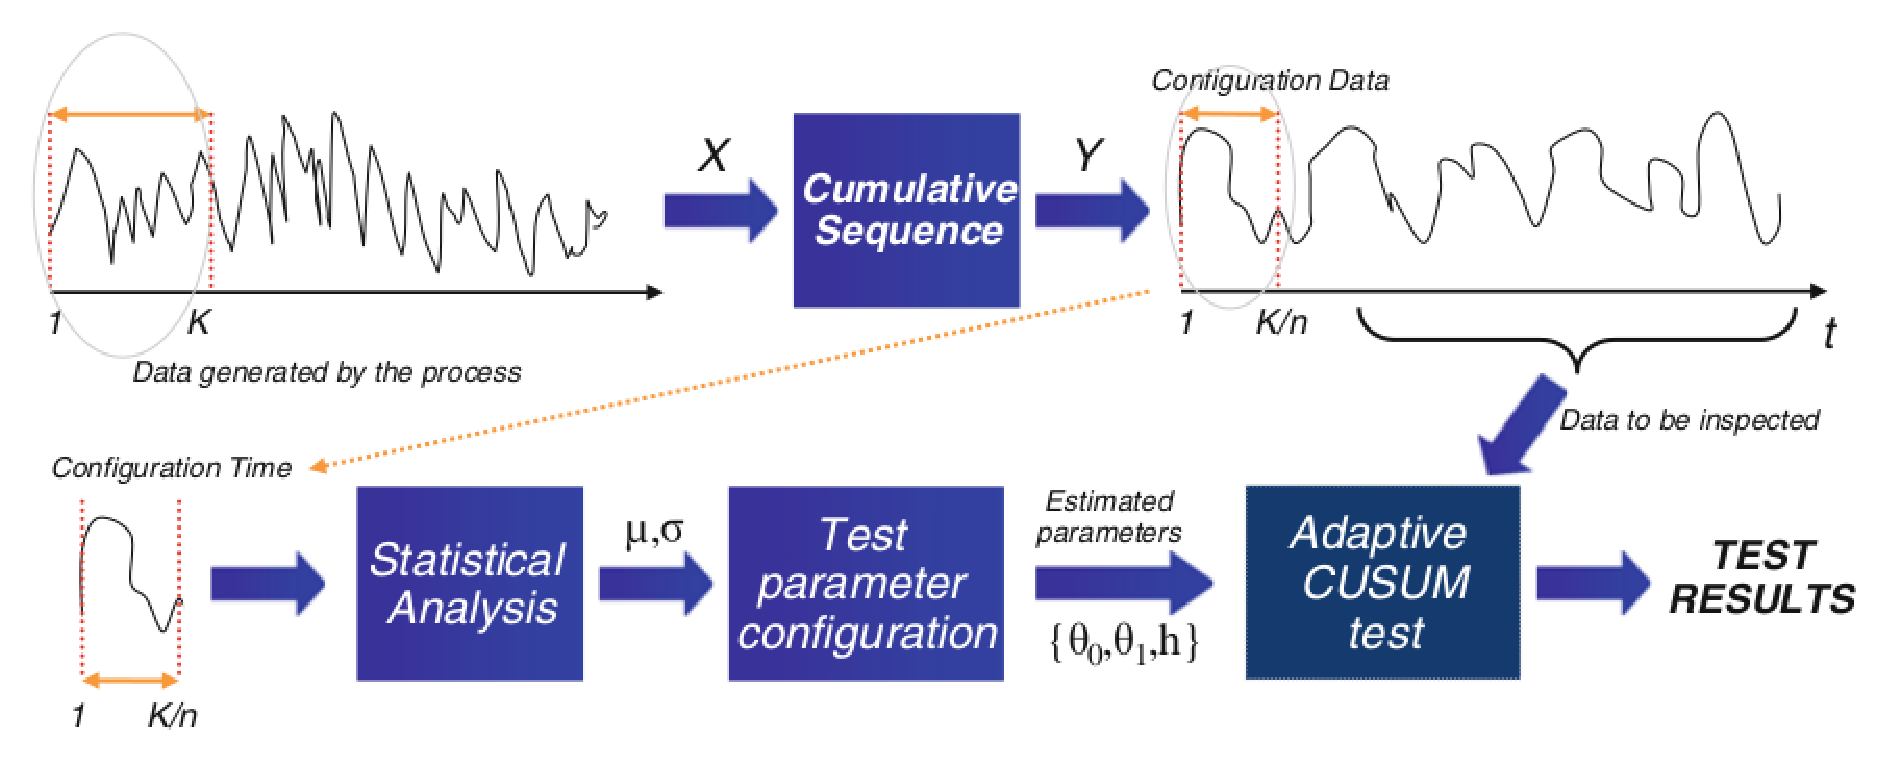
\includegraphics[width=12cm,keepaspectratio]{pictures/adaptiveCUSUM}
	\caption{Procedura del CUSUM
		adattativo}
	\label{fig:adaptiveCUSUM}
\end{figure}
\subparagraph{CI-CUSUM} Il metodo
CI-CUSUM rappresenta un'estensione del
CUSUM adattativo molto potente, in
quanto ciascun descrittore, estratto
dal flusso di dati, pu\`o essere
utilizzato per avere differenti gradi
di sensitivit\`a durante
l'identificazione di un cambiamento.
\begin{figure}
	\centering
	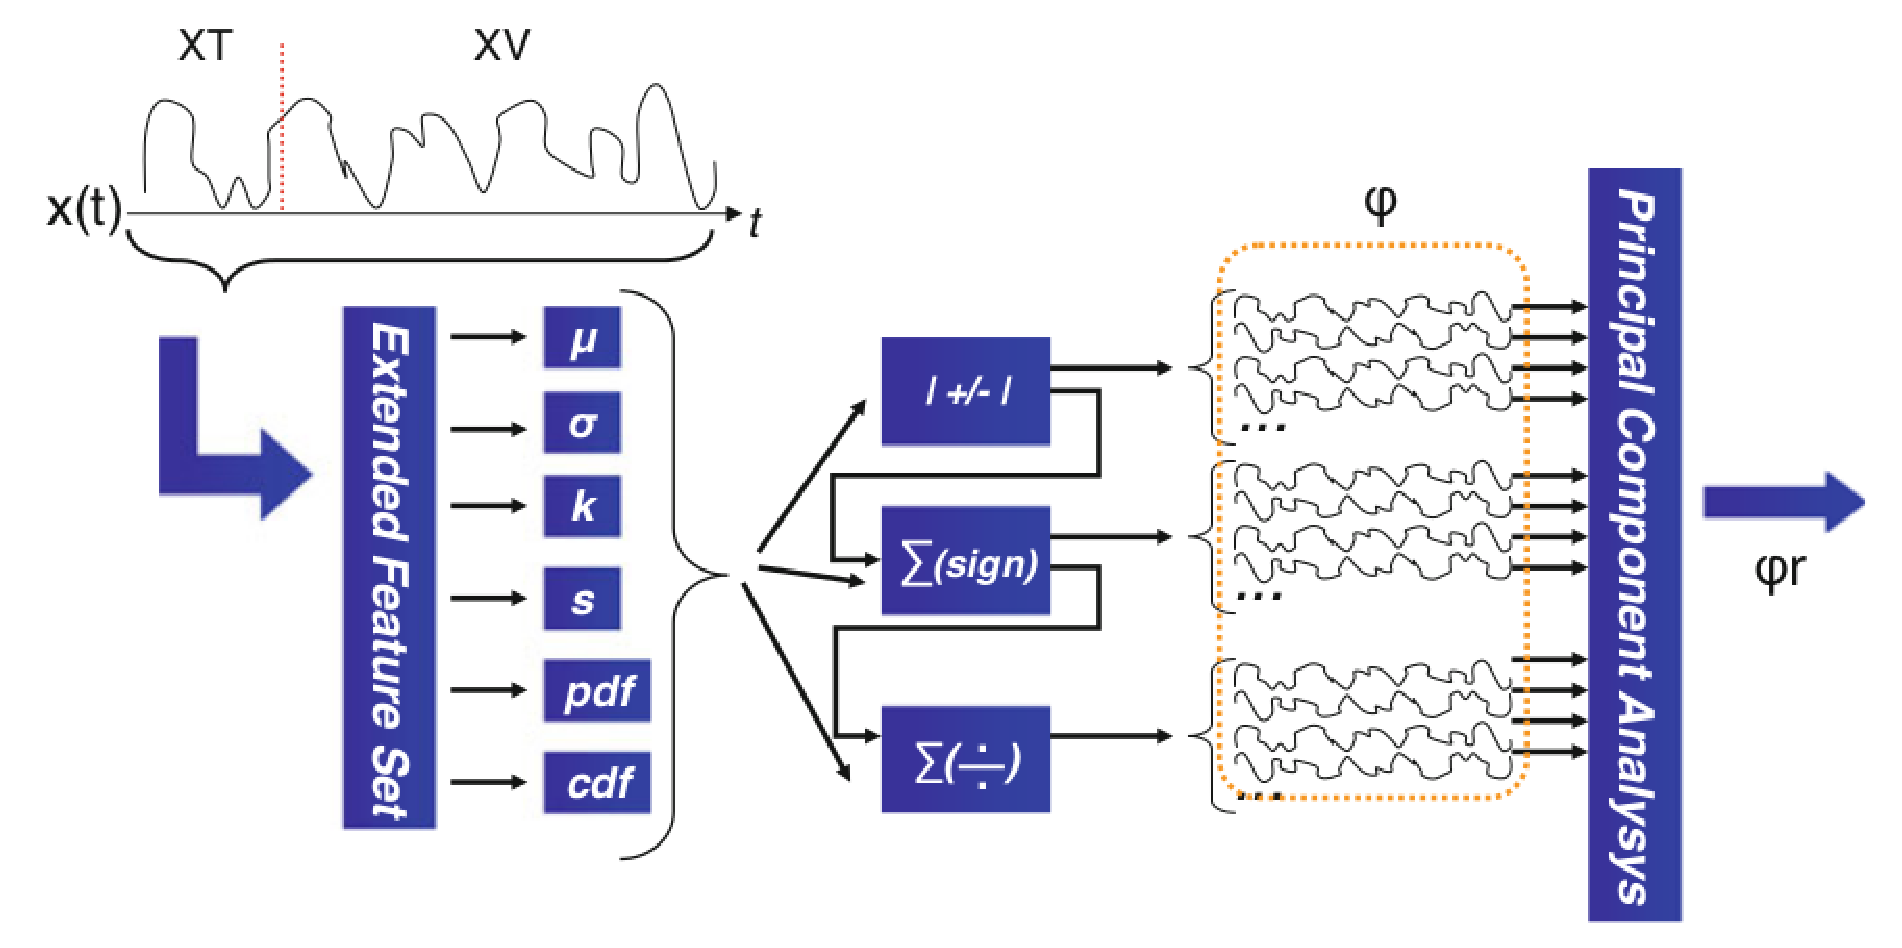
\includegraphics[width=12cm,keepaspectratio]{pictures/CI-CUSUM}
	\caption{Estrazione dei descrittori
		nel metodo CI-CUSUM}
	\label{fig:CI-CUSUM}
\end{figure}
Facciamo riferimento alla Figura \ref{fig:CI-CUSUM}. I descrittori $\varphi$ considerati contengono i principali momenti della distibuzione dei dati, come media e varianza, ma anche momenti superiori al secondo come skewness (\textit{skew}) e kurtosis (\textit{kurt}), oltre che altre informazioni derivate dalla densit\`a probabilistica (\textit{pdf}) e dalla funzione di ripartizione dei dati (\textit{cdf}).\\
A ogni istante queste grandezze
vengono confrontate con quelle
appartenenti all'intervallo di
configurazione (\textit{training set},
indicato in Figura \ref{fig:CI-CUSUM}
come TS), in modo da valutare la
discrepanza tra questi valori. I
descrittori utilizzati sono
\[
\varphi_1(t)=|\mu_0-\mu_V|,\varphi_2(t)=|\sigma_0-\sigma_V|,\]
\[\varphi_3(t)=|\textit{kurt}_0-\textit{kurt}_V|,\varphi_4(t)=|\textit{skew}_0-\textit{skew}_V|, \]
\[\varphi_5(t)=\int_x|\textit{pdf}_0(x)-\textit{pdf}_V(x)|\textit{dx},\]
\[\varphi_6(t)=\int_x|\textit{cdf}_0(x)-\textit{cdf}_V(x)|\textit{dx}, \]
\[ \varphi_{7\leq j\leq 12}(t)=
\sum_{v=1}^{t-1}\textit{sgn}(\varphi_{j-6}(v+1)-\varphi_{j-6}(v)),\]
\[\varphi_{13\leq j\leq 24}(t)=
\sum_{v=1}^{t-1}\frac{\varphi_{j-12}(v+1)}{\varphi_{j-12}(v)} \]
In particolare, i descrittori
$\varphi_5(t)$ e $\varphi_6(t)$
valutano la discrepanza tra la
densit\`a e funzione di ripartizione
correnti e quelle rispettive
dell'intervallo di configurazione. I
descrittori da $\varphi_7(t)$ a
$\varphi_{12}(t)$ vanno ad analizzare
i cambiamenti di segno in elementi
consecutivi e quelli da
$\varphi_{13}(t)$ a $\varphi_{24}(t)$
la somma cumulata del rapporto tra
elementi consecutivi. Per ridurre la
complessit\`a dello spazio dei
descrittori viene applicata
un'\textit{analisi delle componenti
	principali} su $\varphi$, in modo da
avere la trasformata $\varphi_r$. A
questo punto, dato che la
distribuzione di $\varphi_r$ non \`e
nota a priori, viene applicato un
CUSUM adattativo su di essa.
\subsubsection{CDT basati su Intersezione di Intervalli di Confidenza}
La famiglia di tecniche che andiamo ad analizzare adesso \`e in grado di identificare cambi di stazionariet\`a, in un flusso di dati, monitorando l'evoluzione nel tempo di un certo numero di descrittori estratti dai dati stessi.
L'ipotesi principale che viene fatta \`e che le osservazioni della sequenza monitorata siano \textit{indipendenti e identicamente distribuiti} (\textit{i.i.d.}) e generati da una distribuzione \textit{gaussiana}.
\subparagraph{ICI-CDT}
In \textit{ICI-CDT} (Intersection of Confidence Intervals Change Detection Test) \cite{alippi2011just}, i descrittori sono estratti attraverso una \textit{fenestratura} dei dati disponibili in sotto-sequenze composte da $n$ istanze. Per ciascuna sotto-sequenza calcoliamo media e  varianza campionarie che, per il \textit{teorema del limite centrale} \cite{ross2009introduction}, possono essere considerate distribuite in maniera gaussiana. Entrando nel dettaglio, se consideriamo $s$ come l'\textit{s-esima} sotto-sequenza, i descrittori estratti sono:
\[ M(s)=\frac{\sum\limits_{t=(s-1)n+1}^{ns}x(t)}{n} \text{ , e } V(s)=\left(\frac{\left(\sum\limits_{t=(s-1)n+1}^{ns}(x(t)-M(s))^2\right)}{n-1}\right)^{h_0}, \]
dove il parametro $h_0$ \`e un esponente utilizzato per generare un'approssimazione gaussiana della varianza campionaria.\\
ICI-CDT utilizza una prima sequenza dei dati in cui si assume l'assenza di cambiamenti nella distribuzione. Tale sequenza prende il nome di \textit{insieme di training} e viene indicata con $O_{T_0}$. Da questa sequenza viene stimato il parametro $h_0$ e si configura il CDT. La configurazione avviene attraverso le due sequenze di descrittori $\{M(s), s=1,...,S_0\}$ e $\{V(s), s=1,...,S_0\}$, con $S_0=T_0/n$.\\
Calcoliamo quindi le medie $\hat{\mu}^M_{S_0}$, $\hat{\mu}^V_{S_0}$ e le deviazioni standard $\hat{\sigma}^M_{S_0}$, $\hat{\sigma}^V_{S_0}$ dei descrittori nell'insieme di training, ovvero:
\[ \hat{\mu}^M_{S_0}=\frac{\sum\limits_{s=1}^{S_0}M(s)}{S_0} \text{ , e } \hat{\sigma}^M_{S_0}=\sqrt{\frac{\sum\limits_{s=1}^{S_0}(M(s)-\hat{\mu}^M_{S_0})^2}{S_0-1}}, \]
e
\[ \hat{\mu}^V_{S_0}=\frac{\sum\limits_{s=1}^{S_0}V(s)}{S_0} \text{ , e } \hat{\sigma}^V_{S_0}=\sqrt{\frac{\sum\limits_{s=1}^{S_0}(V(s)-\hat{\mu}^V_{S_0})^2}{S_0-1}}. \]
Queste stime definiscono gli \textit{intervalli di confidenza} per i descrittori media e deviazione standard che, sotto la condizione di stazionariet\`a, sono definiti come:
\[I_{S_0}^M= \left[\hat{\mu}^M_{S_0}-\Gamma \hat{\sigma}^M_{S_0} \text{, } \hat{\mu}^M_{S_0}+\Gamma \hat{\sigma}^M_{S_0}\right], \]
\[I_{S_0}^V= \left[\hat{\mu}^V_{S_0}-\Gamma \hat{\sigma}^V_{S_0} \text{, } \hat{\mu}^V_{S_0}+\Gamma \hat{\sigma}^V_{S_0}\right], \]
dove $\Gamma>0$ \`e un parametro che controlla l'ampiezza dell'intervallo di confidenza e, quindi, la probabilit\`a che un descrittore appartenga all'intervallo sotto l'ipotesi di stazionariet\`a. \\
Una volta che la fase di training viene completata, ICI-CDT diventa operativo e pu\`o essere utilizzato per identificare cambiamenti nella stazionariet\`a del flusso di dati. Non appena sono disponibili $n$ dati, viene creata una nuova sequenza $s$ e si calcolano i descrittori che andranno a popolare gli intervalli $I_{s}^{M}$ e $I_{s}^{V}$.\\
A questo punto \`e possibile applicare la \textit{regola dell'intersezione degli intervalli di confidenza} (ICI-rule) \cite{goldenshluger1997spatially}. Questa regola verifica se una nuova istanza di un descrittore possa essere intesa come una realizzazione della gi\`a esistente distribuzione gaussiana. Se ci\`o non viene verificato, allora \`e avvenuto un cambiamento nella distribuzione.\\
Da un punto di vista operazionale, per ciascuna sequenza $s$ vengono calcolati gli intervalli di confidenza dei descrittori come \`e stato fatto per quelli dell'insieme di training. ICI-CDT individua un cambiamento all'interno della sotto-sequenza $\hat{s}$ se
\[\bigcap_{s<\hat{s}}I_s^M \neq \varnothing \text{ e } \bigcap_{s\leq\hat{s}}I_s^M = \varnothing \]
oppure
\[\bigcap_{s<\hat{s}}I_s^V \neq \varnothing \text{ e } \bigcap_{s\leq\hat{s}}I_s^V = \varnothing \]
e il tempo di identificazione $\hat{T}=n\hat{s}$ corrisponde all'ultimo termine della sotto-sequenza $\hat{s}$.\\
\begin{figure}
	\centering
	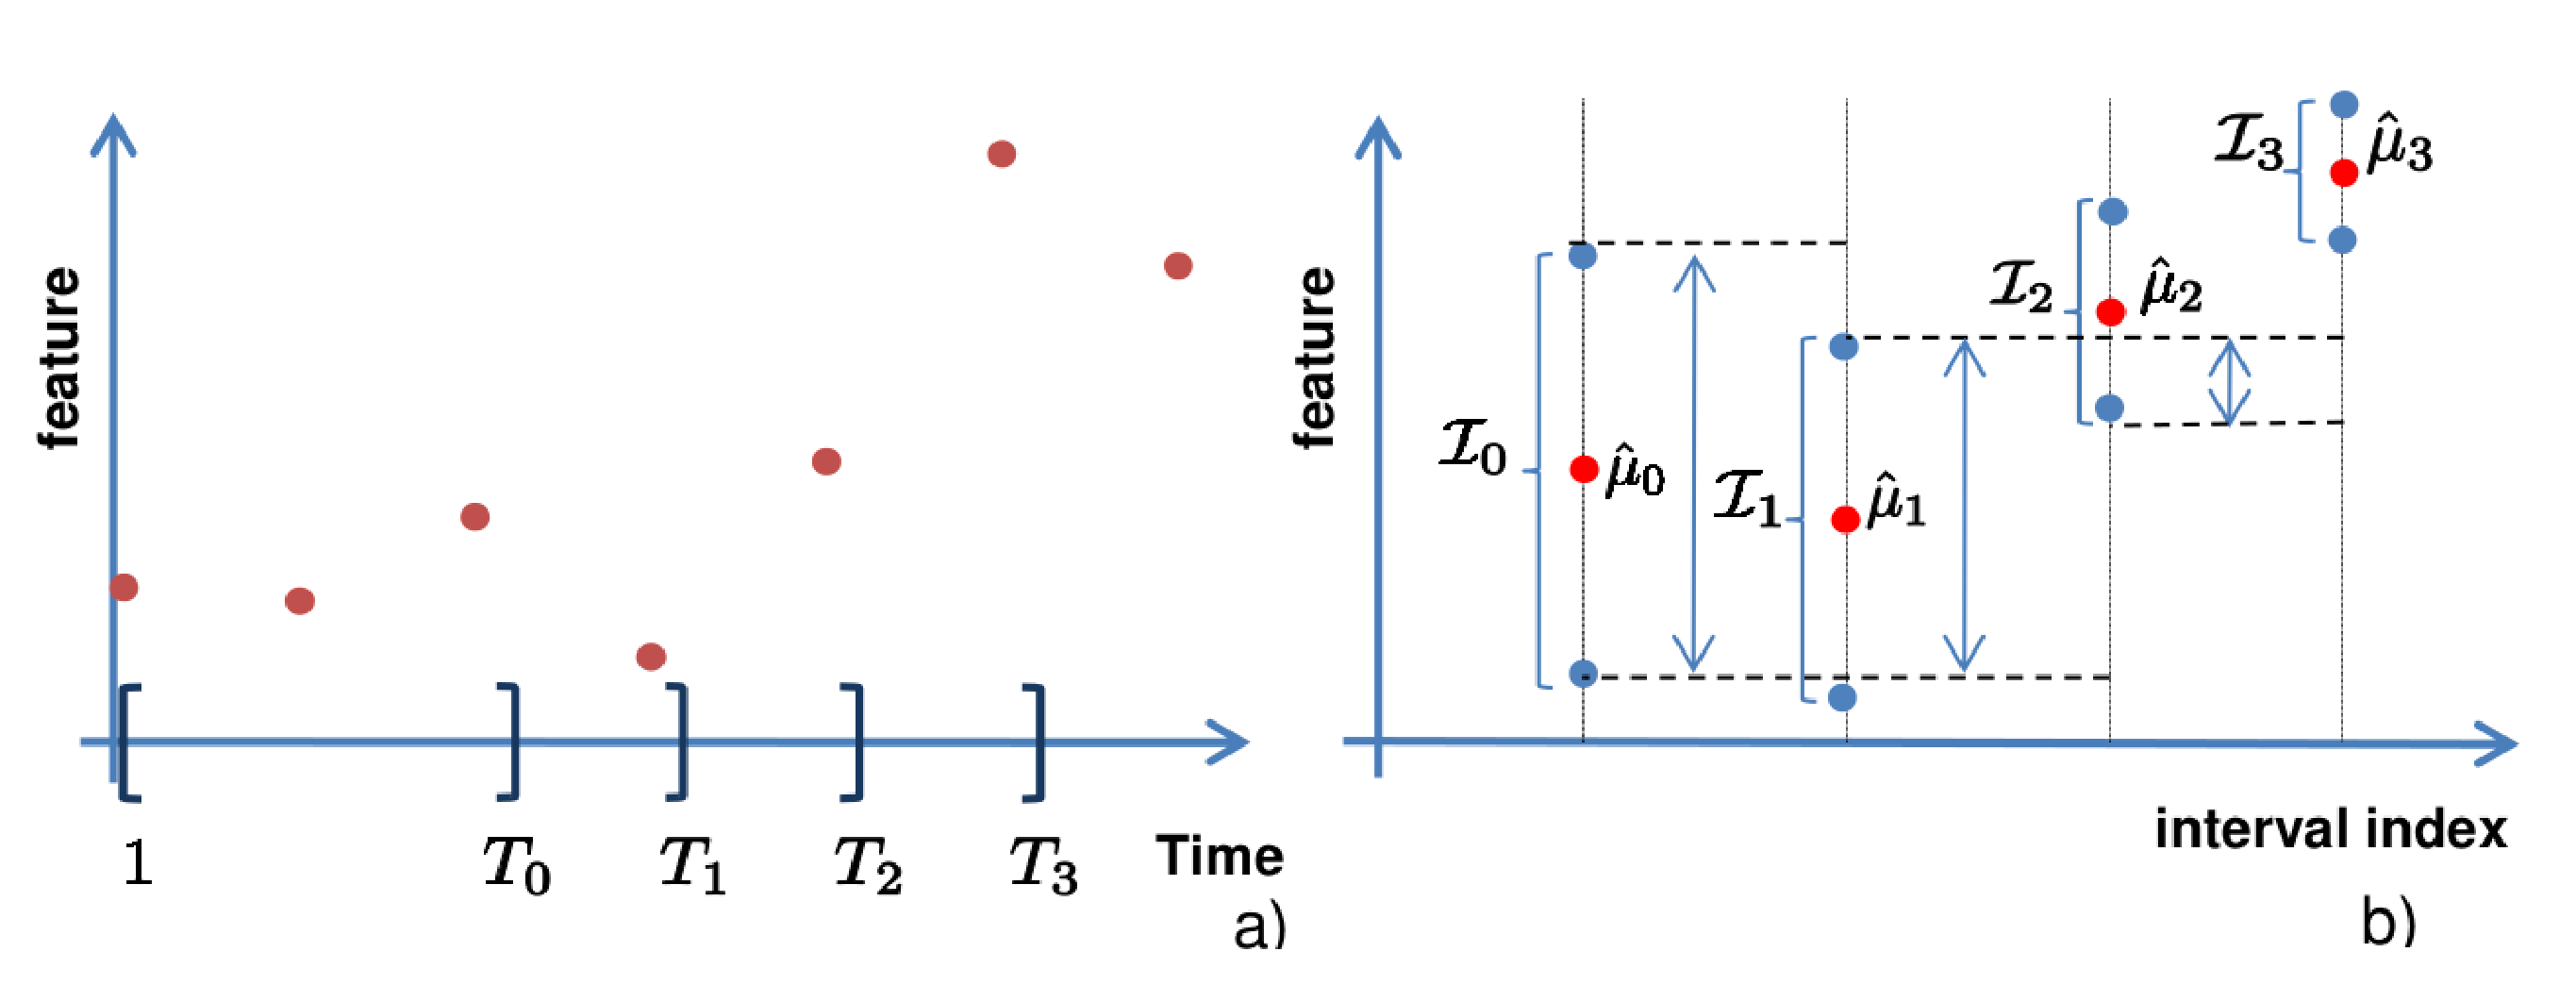
\includegraphics[width=12cm,keepaspectratio]{pictures/ICIrule}
	\caption{Esempio di come opera la regola dell'intersezione degli intervalli di confidenza (ICI-rule)}
	\label{fig:ICIrule}
\end{figure}
La Figura \ref{fig:ICIrule} illustra un esempio di come opera ICI-rule.\\
In \textbf{a} vengono rappresentati i valori dei descrittori e l'insieme di intervalli $\{[1,T_0], [1,T_1], [1,T_2], [1,T_3]\}$, mentre in \textbf{b} sono illustrati gli stimatori delle medie e i loro intervalli di confidenza. In questo caso ICI-rule individua un cambiamento nell'intervallo $[1,T_2]$, dato che $I_0 \cap ...\cap I_2 \neq \varnothing$ e $I_0 \cap ...\cap I_3 = \varnothing$.\\
Il principale problema di questa tecnica consiste nella sua \textit{intrinseca} latenza, dovuta al fatto che opera a finestre. 
Per risolvere questo limite \`e possibile applicare delle trasformazioni sui dati in modo da renderli approssimativamente gaussiani. Le trasformazioni pi\`u utilizzate sono quelle di \textit{Box-Cox}   \cite{box1964analysis}, per dati positivi, e di \textit{Manly}, \cite{manly1976exponential} che pu\`o essere utilizzato anche per dati negativi. Usando questo tipo di trasformazioni possiamo evitare di lavorare a finestre e utilizzare un approccio \textit{elemento  per elemento} \cite{boracchi2014reconfigurable}.           
\subparagraph{CDT di tipo gerarchico} 
Un altro problema di ICI-CDT consiste nel fatto che esso genera un numero molto elevato di falsi positivi. Per fare in modo che questo numero si abbassi, impattando il meno possibile sul tempo di esecuzione, \`e possibile fare un CDT di tipo \textit{gerarchico} \cite{alippi2011hierarchical}, basato su due livelli:
\begin{itemize}
	\item Il primo livello \`e composto da ICI-CDT, e opera sequenzialmente su tutti i dati.
	\item Il secondo livello consiste in un test d'ipotesi statistico in grado di validare o rifiutare l'ipotesi di avvenuto cambiamento. Questo livello viene attivato ogni volta che viene identificato un cambiamento da ICI-CDT.
\end{itemize}
\begin{figure}
	\centering
	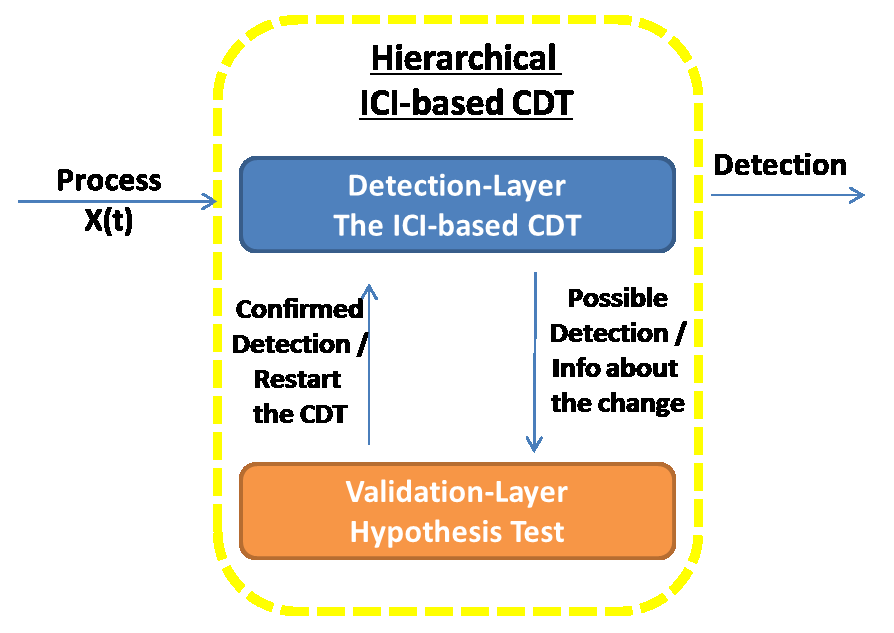
\includegraphics[width=8cm,keepaspectratio]{pictures/Hierarchical_ICI_based_CDT_Scheme}
	\caption{Schema del modo di operare del CDT di tipo gerarchico}
	\label{fig:HierarchicalCDT}
\end{figure}
Uno schema di come opera questo tipo di CDT \`e visualizzato nella Figura \ref{fig:HierarchicalCDT}.
Il CDT di tipo gerarchico \`e progettato in modo da avere un primo livello molto efficiente dal punto di vista del tempo di esecuzione, anche se ci\`o si traduce in un numero elevato di falsi positivi. Questo limite viene mitigato usando nel secondo livello della gerarchia un test pi\`u efficiente dal lato del numero di falsi positivi prodotti. Il fatto che il secondo livello ha un tempo di esecuzione maggiore non \`e un problema, in quanto esso viene attivato solamente nei casi in cui il primo livello della gerarchia segnala un possibile cambiamento nella distribuzione dei dati.
\section{Tampering Detection}
\label{tamperingSOA}
Nei moderni sistemi di videosorveglianza troviamo spesso algoritmi in grado di identificare particolari eventi all'interno della scena ripresa dalla camera. 
Ad esempio \`e possibile avere un software in grado di identificare le targhe delle automobili che superano il limite di velocit\`a, oppure la presenza di oggetti incustoditi in una stazione \cite{Targhe}.
Affinch\'e questi algoritmi funzionino correttamente, \`e importante che l'\textit{affidabilit\`a} del sistema di acquisizione sia preservata.
Questa propriet\`a viene soddisfatta quando:
\begin{itemize}
	\item la camera mantiene la stessa inquadratura nell'area di interesse;
	\item tutti gli elementi della scena sono distinguibili all'interno dell'immagine.
\end{itemize}
%In un'applicazione di monitoraggio video consideriamo che la camera, in condizioni di funzionamento ottimale, mantenga la stessa inquadratura nel tempo e che sia in grado di acquisire, in maniera nitida, tutti gli elementi di interesse presenti nella scena.
Definiamo \gls{tampering} un qualsiasi evento che determini un cambio di inquadratura o che non permetta la corretta acquisizione di una parte o della totalit\`a della scena.
Possiamo classificare gli eventi di tampering in quattro categorie:
\begin{itemize}
	\item sfocature,
	\item spostamenti della camera,
	\item occlusioni dell'obiettivo,
	\item guasti della camera.
\end{itemize}
La letteratura scientifica presenta molte tecniche in grado di affrontare il problema dell'identificazione di questo tipo di eventi.
%Per affrontare il problema dell'identificazione di questo tipo di eventi, la letteratura scientifica offre molte tecniche che permettano l'identificazione automatica di eventi in grado di compromettere la corretta ripresa della scena da parte della videocamera.
\begin{figure}[tb]
	\centering
	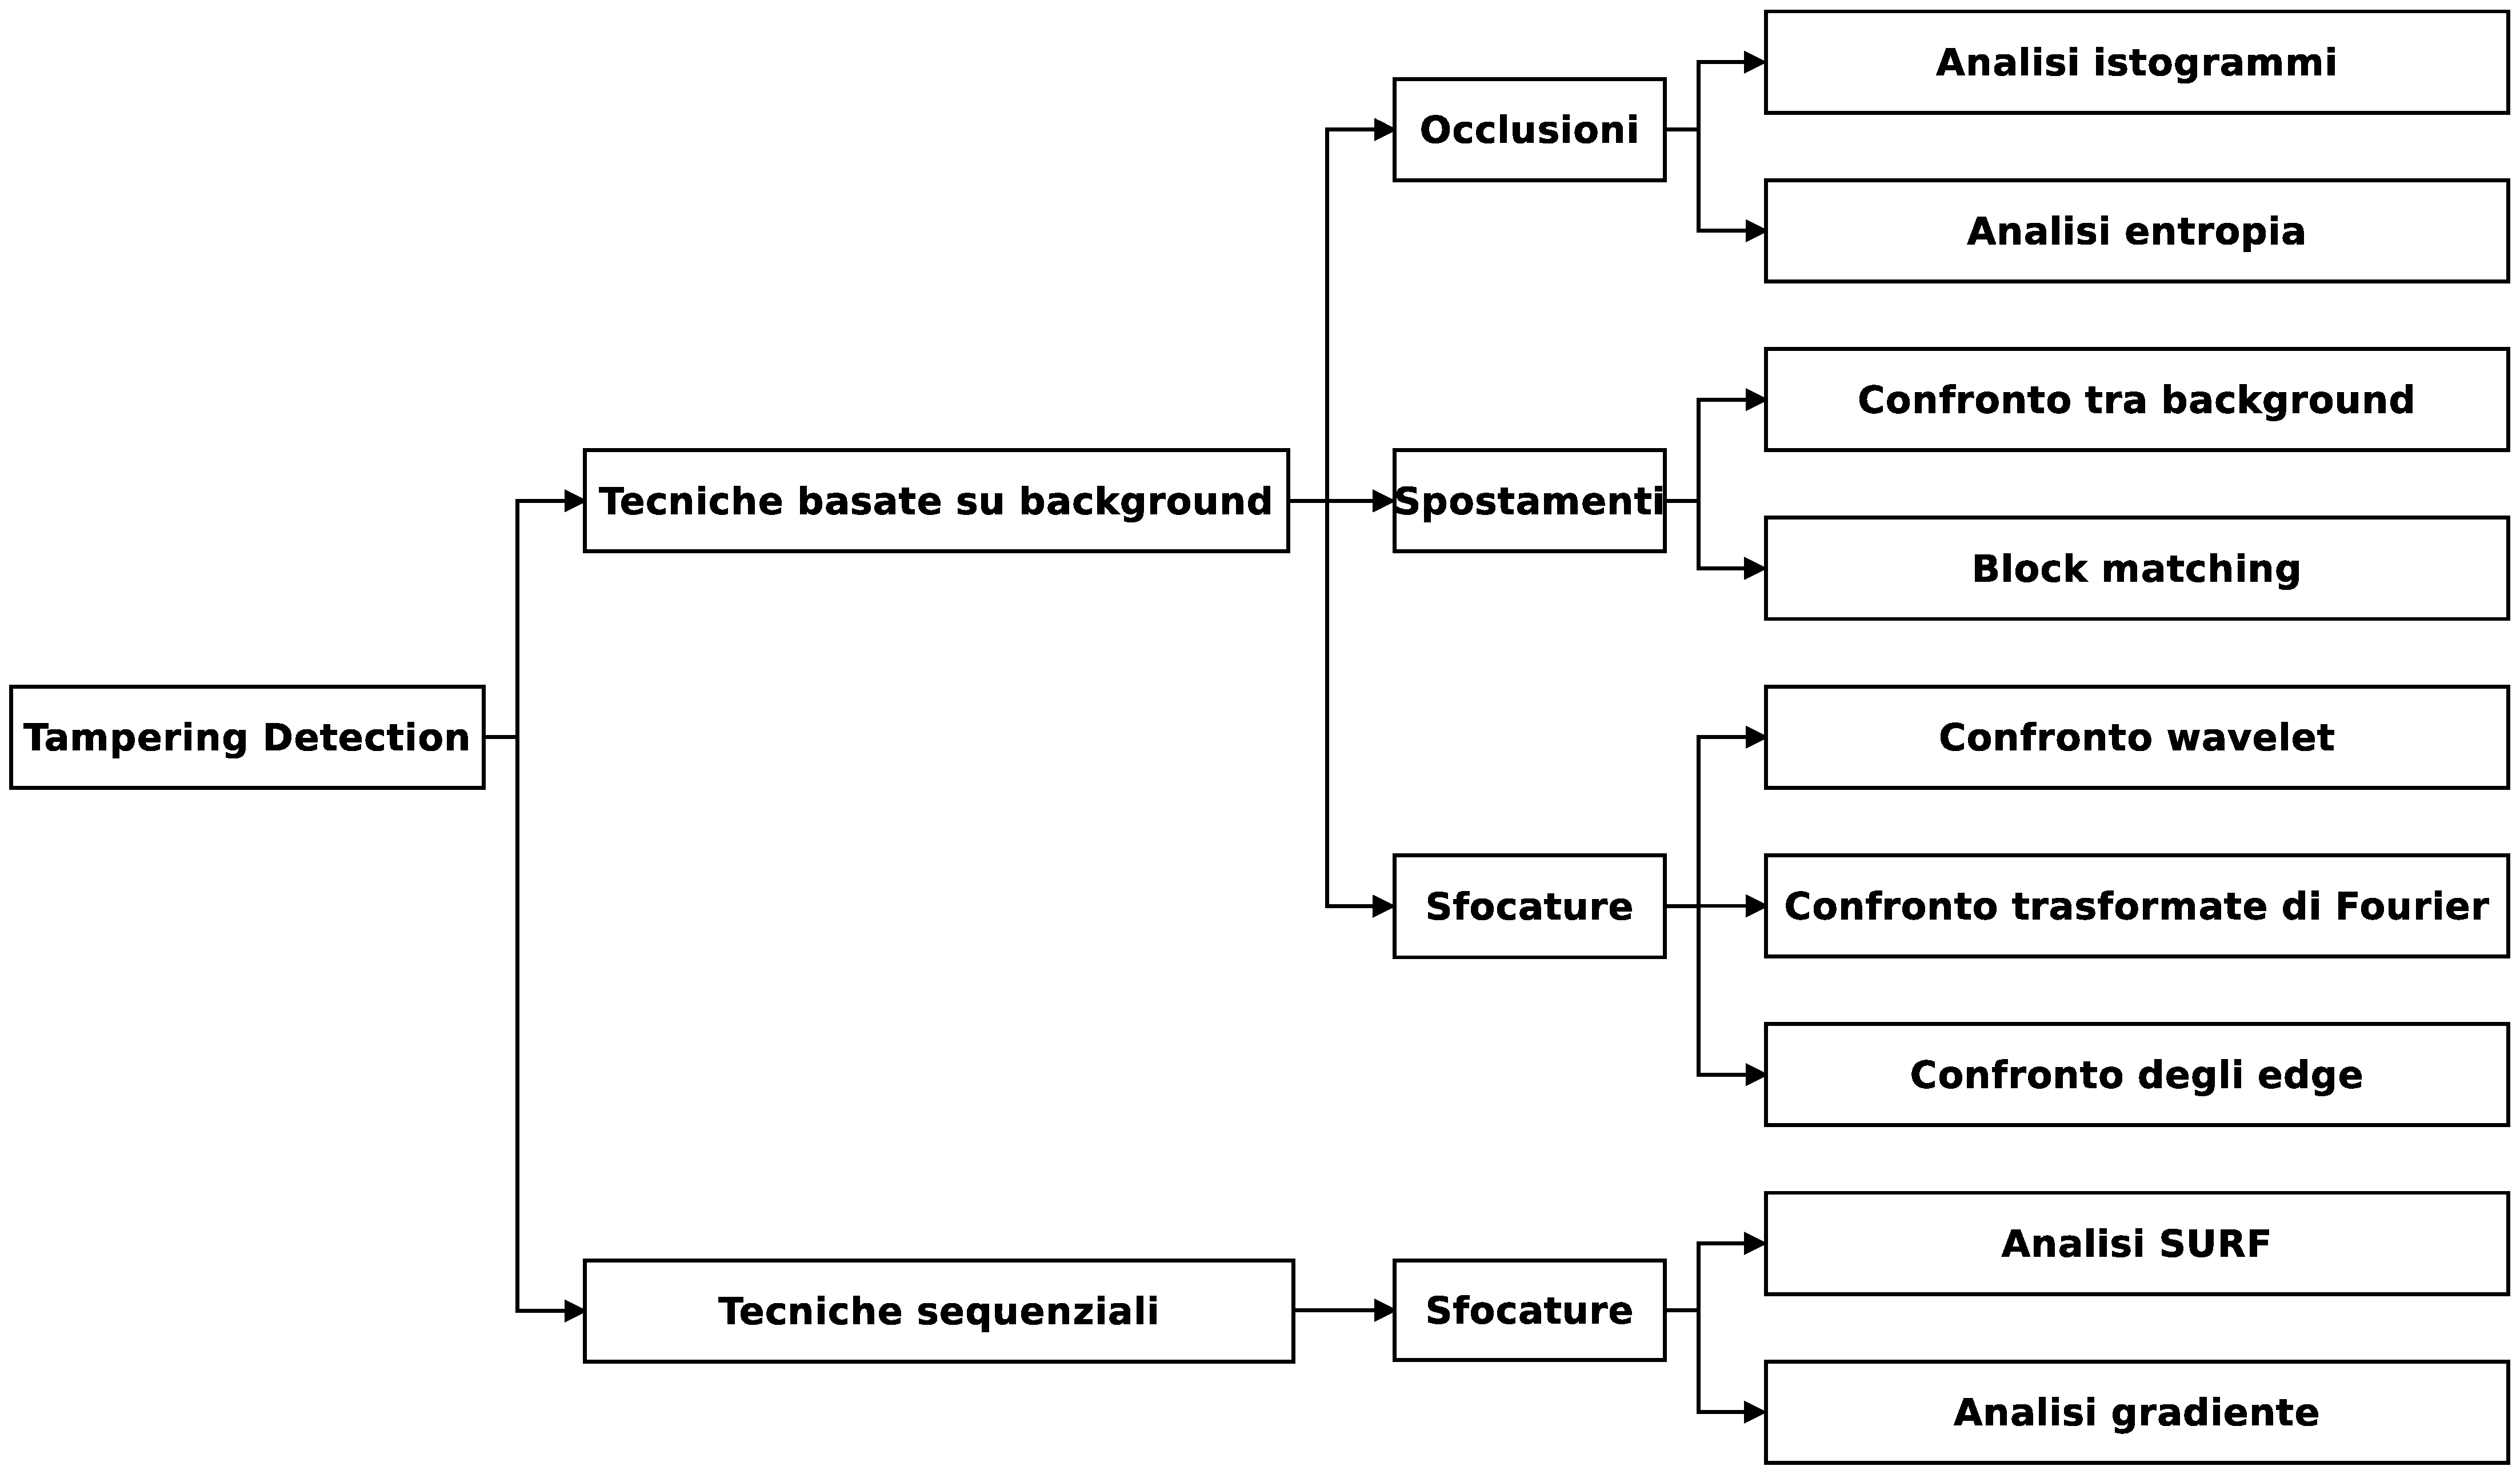
\includegraphics[width=12cm]{./diagrammi/tecnicheSOA.eps}
	\caption{Tecniche di tampering detection}
	\label{fig:tamperingSOA}
\end{figure}
Lo schema in Figura \ref{fig:tamperingSOA} mostra le principali tecniche di tampering detection presenti in letteratura.
Queste possono essere divise in due categorie: 
\begin{itemize}
	\item tecniche basate su confronto di background,
	\item tecniche basate su monitoraggio sequenziale.
\end{itemize}
Nel seguito del paragrafo verranno descritti i principali metodi utilizzati in queste due categorie.
\subsection{Concetti e terminologia}
\label{concetti}
Prima di concentrarci su come \`e stato affrontato il problema del tampering detection, definiamo i concetti e i termini che verranno utilizzati nel seguito della trattazione.\\
Lo scenario che consideriamo \`e quello di una camera che deve riprendere una particolare \textit{\gls{scena}}.
\begin{figure}[tb]
	\centering
	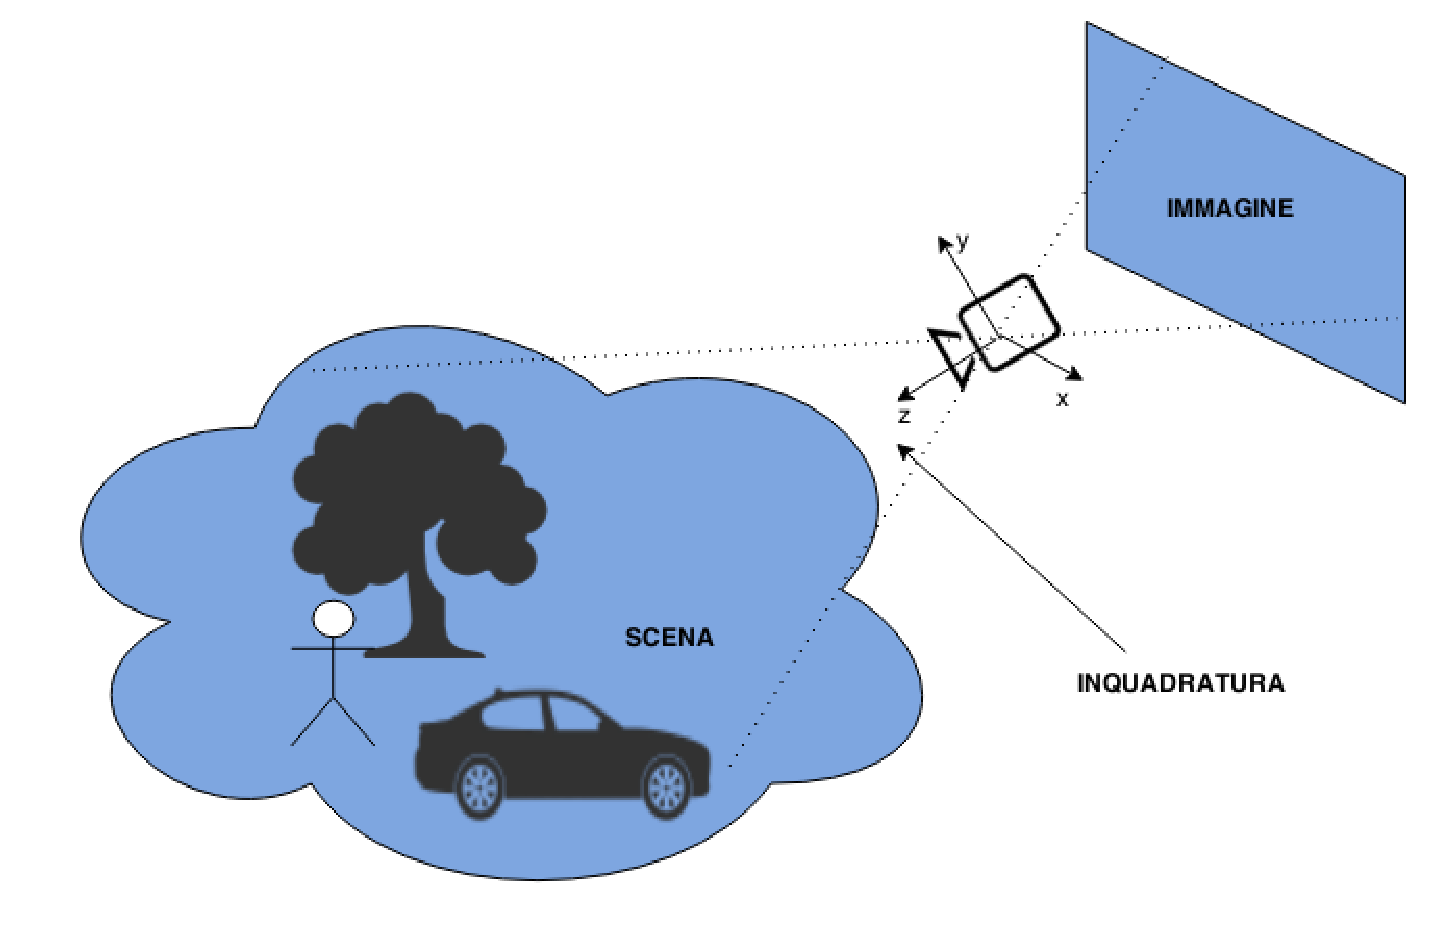
\includegraphics[width=12cm]{./pictures/videoMonitoring}
	\caption{Sistema di monitoraggio video}
	\label{fig:videoMonitoring}
\end{figure}
\noindent 
La posizione e l'orientamento della camera determinano l'\textit{\gls{inquadratura}} della scena.
L'acquisizione, da parte della camera, della scena nell'istante di tempo $t$ viene definita \textit{immagine} o \textit{frame} $t$-esimo.
La Figura \ref{fig:videoMonitoring} illustra questi concetti.\\
Per semplificare la trattazione, considereremo immagini estratte in \textit{scala di grigi}.
Ciascuna immagine, quindi, verr\`a rappresentata come una matrice di pixel, in cui ciascun elemento rappresenta l'intensit\`a luminosa (\textit{luma}) del pixel corrispondente.
L'estensione al caso di immagini \textit{RGB} \`e immediata: possiamo, infatti, applicare i vari algoritmi in maniera indipendente per ciascun canale di colore, per poi mediare i risultati ottenuti.\\
Nel seguito della trattazione useremo una specifica terminologia.
Indicheremo con $\mathcal{X}$ l'insieme dei \textit{pixel} costituenti l'immagine acquisita dalla camera,
\[ \mathcal{X} \subset \mathbb{N}^2, \]
e con $x \in \mathcal{X}$ il singolo pixel.
Quando vorremo considerare il frame acquisito all'istante di tempo $t$, useremo $z_t$, con $t=1,\dots , \infty$. 
In particolare, per indicare il valore della \textit{luminosit\`a} del pixel $x$ per il frame $t$-esimo, useremo il termine $z_t(x)$, con 
\[ z_t(x) \in [0, 255] \forall x \in \mathcal{X}. \]

\subsection{Tecniche basate su confronto di background}
\label{background}
Nella maggior parte dei lavori dedicati al problema del tampering detection, il metodo principalmente utilizzato consiste nel confrontare ciascun frame con un modello che viene calcolato a partire dalle osservazioni precedenti.
Tale metodo \`e ampiamente utilizzato in vari ambiti della visione artificiale e prende il nome di \textit{background subtraction}.
Una tecnica generale di calcolo del background \`e presentata in \cite{aksay2007camera}.
%Indichiamo con $z_i(x)$ il valore, nel pixel $x$, della luminosit\`a nell'$i$-esimo frame.
Il valore del modello di background per il pixel $x$\ \`e calcolato, in maniera ricorsiva, secondo la seguente formula:
\[
\label{eq:background}
B_{t + 1}(x)=\left\{ \begin{array} {lcl}
aB_t(x)+ (1-a)z_t(x) \\
\mbox{\hspace{1.5cm}, se } |z_t(x) - z_{t-1}(x)|\leq T_t(x) \\
B_t(x) \mbox{\hspace{0.5cm}, se } |z_t(x) - z_{t-1}(x)|>T_t(x)\end{array} \right. , \forall x \in \mathcal{X},
\]
dove $0 < a < 1$ \`e chiamato \textit{parametro di aggiornamento} (\textit{update parameter}) e $\Gamma_t(x)$ \`e una soglia che permette di identificare un cambiamento sostanziale di luminosit\`a nel pixel $(x)$. 
 Questa soglia viene aggiornata in maniera ricorsiva secondo la seguente formula:
  \[
  \label{eq:backgroundThreshUpd}
  \Gamma_{t + 1}(x)=\left\{ \begin{array} {lcl}
  a\Gamma_t(x)+ (1-a)(c |z_t(x) - B_t(x)|) \\
  \mbox{\hspace{1.5cm}, se	}  |z_t(x) - z_{t-1}(x)|\leq \Gamma_t(x) \\
  \Gamma_t(x) \mbox{	\hspace{0.5cm}, se	}  |z_t(x) - z_{t-1}(x)|>\Gamma_t(x) \end{array} \right. ,\forall x \in \mathcal{X},
  \]
  dove $c > 1$ e $0<a<1$.
  Lo stesso modello viene utilizzato in altri lavori, come ad esempio in \cite{saglam2009real} e \cite{tsesmelis2013tamper}, mentre una variante molto usata consiste nel calcolare il modello di background a partire dall'\textit{estrazione dei contorni} di ciascun frame (\cite{harasse2004automated}, \cite{gil2007automatic}).
  Un approccio diverso, ma comunque riconducibile allo stesso filone, lo troviamo in \cite{ribnick2006real}, dove il background \`e sostituito da un \textit{buffer} contenente gli ultimi $n$ frame acquisiti dalla camera, che vengono confrontati con l'ultima osservazione per identificare eventi di tampering.
\subsubsection{Identificazione di occlusioni}
L'evento di occlusione avviene quando un oggetto opaco viene posto vicino alla camera, in modo da coprire la scena ripresa.
In \cite{aksay2007camera} e \cite{saglam2009real} questo evento \`e associato a un cambiamento nella struttura dell'\textit{istogramma} del frame occluso rispetto a quello del background.
In particolare, se $z_t$ \`e un frame in cui \`e avvenuta un'occlusione, ci si aspetta che il suo istogramma contenga i valori pi\`u alti in un intervallo pi\`u ristretto rispetto a quello del background $B_t$, in quanto la maggior parte dell'immagine prender\`a il colore dell'oggetto occludente o diventer\`a pi\`u scura.\\
Indichiamo con $H_b(\cdot)$ il valore del $b$-esimo bin dell'istogramma di un frame, con $1 \leq b \leq 32$.
Per identificare un evento di occlusione vengono considerate due disequazioni:
\begin{eqnarray}
 \left(H_{max\left(H(z_t)\right)-1}(z_t) + H_{max\left(H(z_t)\right)}(z_t) +  H_{max\left(H(z_t)\right) + 1}(z_t)\right) \nonumber \\
 > \Gamma_1 \left(H_{max\left(H(z_t)\right)-1}(B_t) + H_{max\left(H(z_t)\right)}(B_t)
  +  H_{max\left(H(z_t)\right) + 1}(B_t)\right), \nonumber
\end{eqnarray}
\[ \sum_{b=1}^{32} H_b\left(|z_t - B_t|\right) > \Gamma_2 \sum_{b=1}^{k}H_b\left(|z_t - B_t|\right),\]
dove $\Gamma_1 > 1$, $\Gamma_2 > 1$ e $0 \leq k < 32$ sono soglie che possono essere modificate in base alla sensibilit\`a che si richiede da parte dell'algoritmo.\\
%In particolare, $\Gamma_1$ e $\Gamma_2$ possono essere aumentate in modo da aumentare la sensibilit\`a, mentre $k$ pu\`o essere diminuito.\\
Un approccio simile \`e presente in \cite{harasse2004automated}, \cite{gil2007automatic} e \cite{ellwart2012camera}, in cui l'evento di occlusione \`e associato a un abbassamento dell'\textit{entropia}:
 \[
 \label{eq:entropy}
 E=-\sum_{k}p_k\ln(p_k) ,
 \]
 dove $p_k$ rappresenta la probabilit\`a che il livello di grigio $k$ sia presente all'interno dell'immagine. \\
 Per riuscire a identificare delle occlusioni \textit{parziali} le tecniche descritte sopra non sono efficaci, in quanto tali eventi non sono in grado di modificare in maniera sostanziale la struttura dell'istogramma dei frame.
 Una soluzione (\cite{gil2007automatic}) consiste nel dividere ciascuna immagine in un certo numero di \textit{blocchi} della stessa dimensione, in modo da applicare le tecniche descritte sopra per ciascuna partizione.
\subsubsection{Identificazione di spostamenti della camera}
Quando viene spostata la camera, in modo cambi l'inquadratura della scena, l'immagine di background $B_i$ viene lentamente aggiornato in modo da riflettere i cambiamenti avvenuti nei frame. 
In \cite{saglam2009real} il metodo proposto per identificare uno spostamento della camera consiste nel confrontare l'immagine di background $B_t$ con $B_{t-k}$, ovvero con un secondo modello \textit{ritardato} di $k$ frame, dove $k \in \mathbb{Z}^+$.
L'approccio consiste nel calcolare un \textit{valore di proporzione} $P$, ottenuto dal confronto tra i due modelli:
\[
\label{eq:displEqSaglam}
P=\left\{ \begin{array} {lcl}
P+1 & \mbox{, se} & B_t(x) \neq B_{t-k}(x) \\
P & \mbox{, se} & B_t(x) = B_{t-k}(x) \end{array} \right. .
\]
Lo spostamento della camera viene identificato quando $P > \Gamma \cdot K$, dove $0<\Gamma<1$ \`e un valore di soglia scelto in base alla sensibilit\`a che si vuole dare all'algoritmo e $K$ \`e il numero totale di pixel dell'immagine.\\
Un altro approccio \`e quello di utilizzare tecniche di \textit{block matching}.
L'algoritmo di block matching fornisce due parametri:
il primo parametro, $m$, indica il \textit{vettore della traslazione} tra il background e il frame corrente, mentre il secondo parametro \`e lo ZNCC relativo a quel vettore.
In \cite{gil2007automatic} e \cite{harasse2004automated} l'algoritmo calcola il vettore di spostamento $m$ del frame corrente rispetto al background, e calcola la \textit{zero-mean normalized cross correlation} (ZNCC) \cite{roma2002comparative}:
\[
ZNCC_t(m) = \frac{\sum_{x \in \mathcal{X}}(B_{t-1}(x)- \mu_{B_{t-1}})(z_t(x+m)-\mu_{z_t})}{\sigma_{B_{t-1}} \sigma_{z_t}},
\]
dove $\mu_{z_t}$ e $\sigma_{z_t}$ rappresentano la media e la deviazione standard della luminosit\`a nell'immagine $z_t$.
Lo spostamento viene individuato quando il vettore $m$ ha una lunghezza minima e lo ZNCC corrispondente supera una certa soglia.
Un metodo simile viene utilizzato anche in \cite{kryjak2012fpga}, con la differenza che, invece di analizzare la correlazione dei pixel, viene analizzata quella degli istogrammi. 
\subsubsection{Identificazione di sfocature} 
La conseguenza di un evento di sfocatura \`e la perdita di dettagli nell'immagine.
In \cite{aksay2007camera} e \cite{saglam2009real} questo fenomeno \`e associato a una diminuzione dell'energia ad alta frequenza. 
Per analizzare questo cambiamento, \cite{aksay2007camera} confronta ciascun frame con il background nel dominio delle \textit{wavelet} \cite{mallat1989theory}, mentre \cite{saglam2009real} utilizza il dominio della \textit{trasformata di Fourier} \cite{bracewell1978fourier}.
\begin{figure}[tb]
	\centering
	\begin{subfigure}[]
		{\label{fig:defocusNormale} 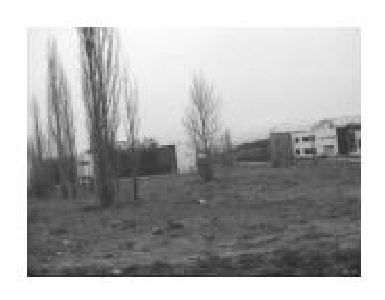
\includegraphics[width = 5cm]{./pictures/normale}}
	\end{subfigure}
	\begin{subfigure}[]
		{\label{fig:defocusNormaleFourier} 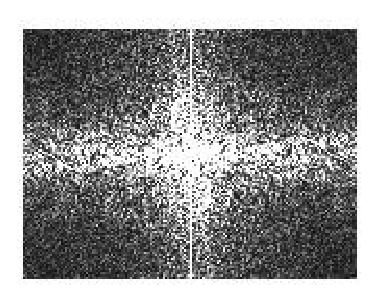
\includegraphics[width = 5cm]{./pictures/normale-fourier}}
	\end{subfigure}
	\begin{subfigure}[]
		{\label{fig:defocusSfocato} 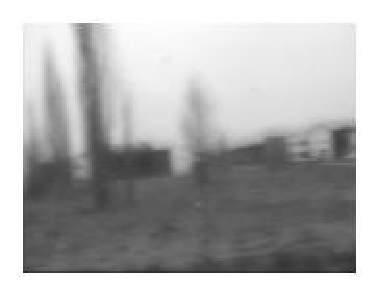
\includegraphics[width = 5cm]{./pictures/sfocato}}
	\end{subfigure}
	\begin{subfigure}[]
		{\label{fig:defocusSfocatoFourier} 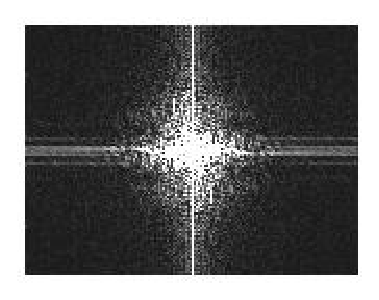
\includegraphics[width = 5cm]{./pictures/sfocato-fourier}}
	\end{subfigure}
	\caption{Comportamento della trasformata di Fourier nel caso di sfocatura}
	\label{fig:fourier}
\end{figure}
Nella Figura \ref{fig:fourier} vediamo un esempio di come si comporta la trasformata di Fourier nel caso di sfocature: 
nel passaggio da un frame nitido (Fig. \ref{fig:defocusNormale}) a uno sfocato (Fig. \ref{fig:defocusSfocato}) abbiamo un crollo delle componenti ad alta frequenza nelle trasformate di Fourier (rispettivamente Fig. \ref{fig:defocusNormaleFourier} e Fig. \ref{fig:defocusSfocatoFourier}).
L'evento di tampering viene individuato quando l'\textit{energia media} della trasformata di Fourier (o di quella wavelet) del frame corrente $E_{HF}(z_t)$ \`e $\Gamma$ volte minore di quella del background $E_{HF}(B_t)$:
\[E_{HF}(z_t)\leq \Gamma \cdot E_{HF}(B_t),\]
dove $0<\Gamma<1$ \`e  un valore di soglia scelto in base alla sensibilit\`a che si vuole dare all'algoritmo.\\
\begin{figure}[tb]
	\centering
	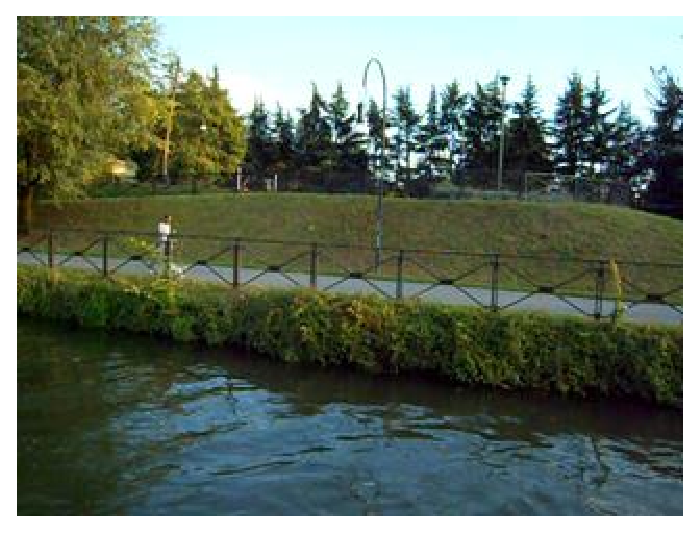
\includegraphics[width = 4cm]{./pictures/FPSalto/img0001}
	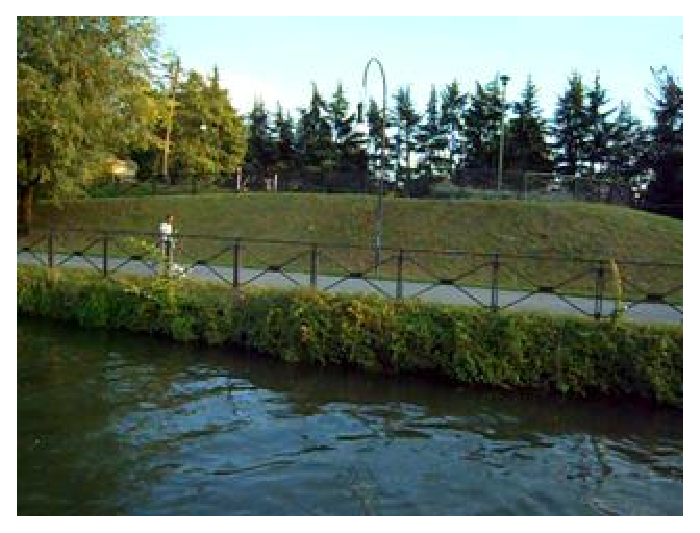
\includegraphics[width = 4cm]{./pictures/FPSalto/img0002}
	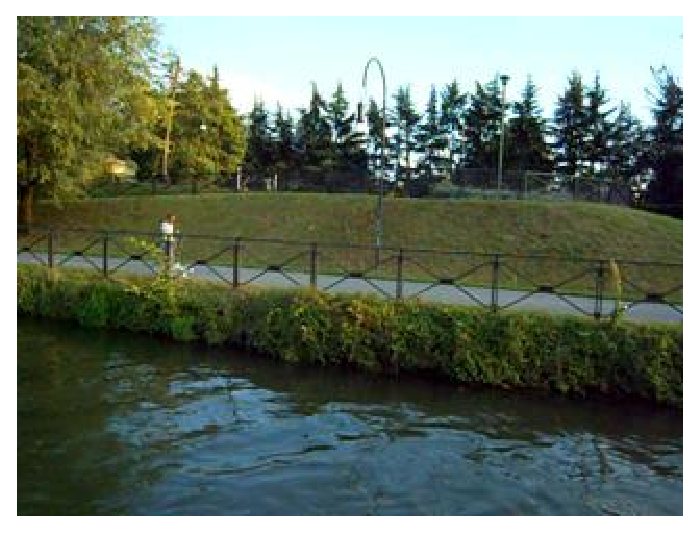
\includegraphics[width = 4cm]{./pictures/FPSalto/img0003}
	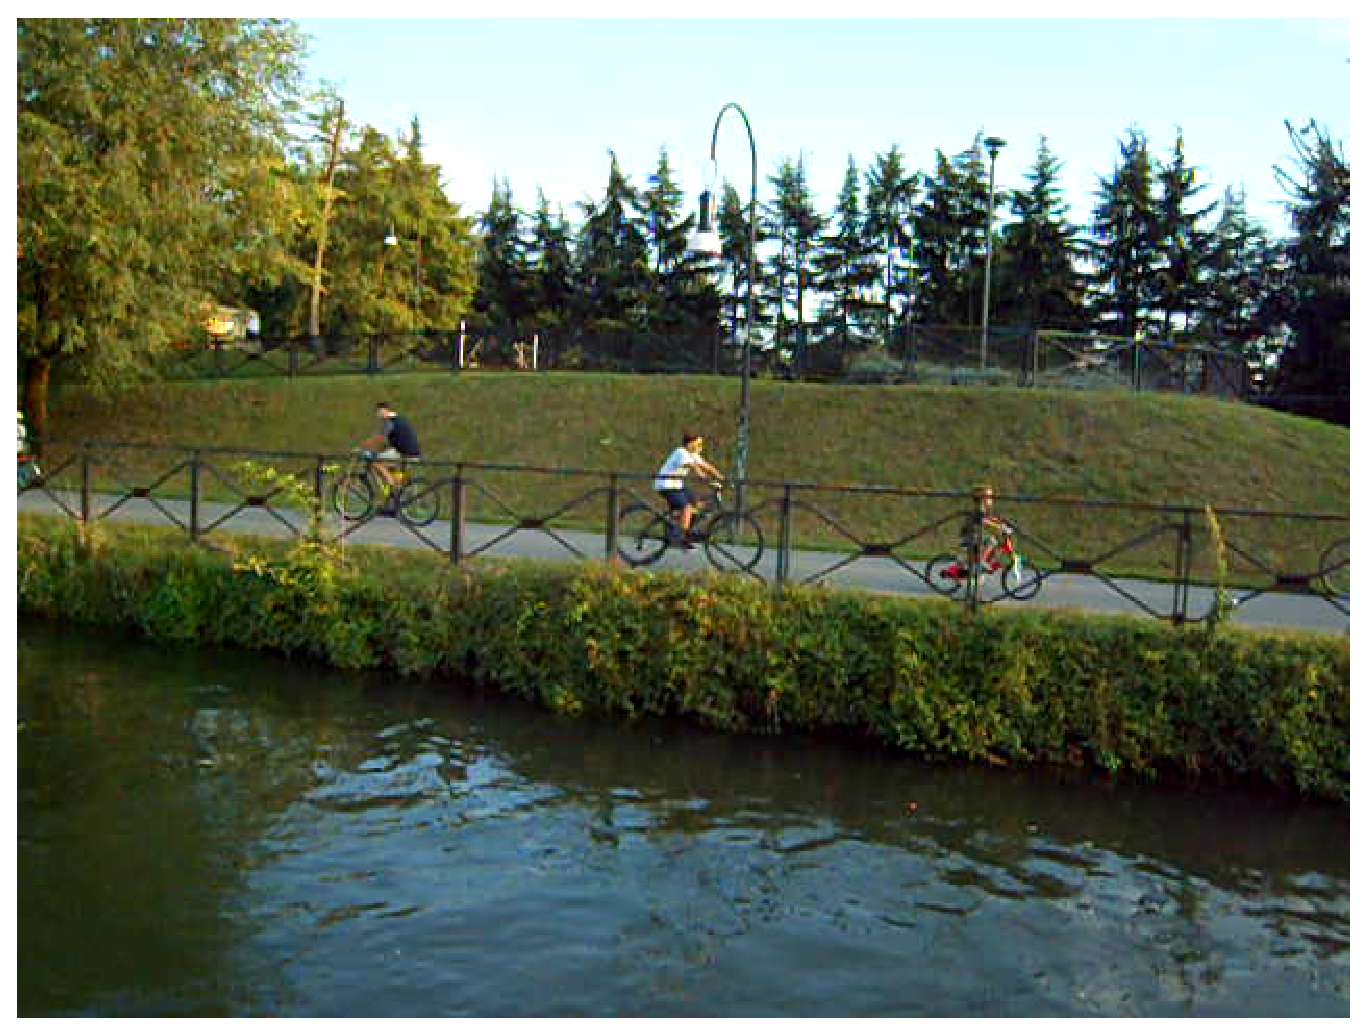
\includegraphics[width = 4cm]{./pictures/FPSalto/img0004}
	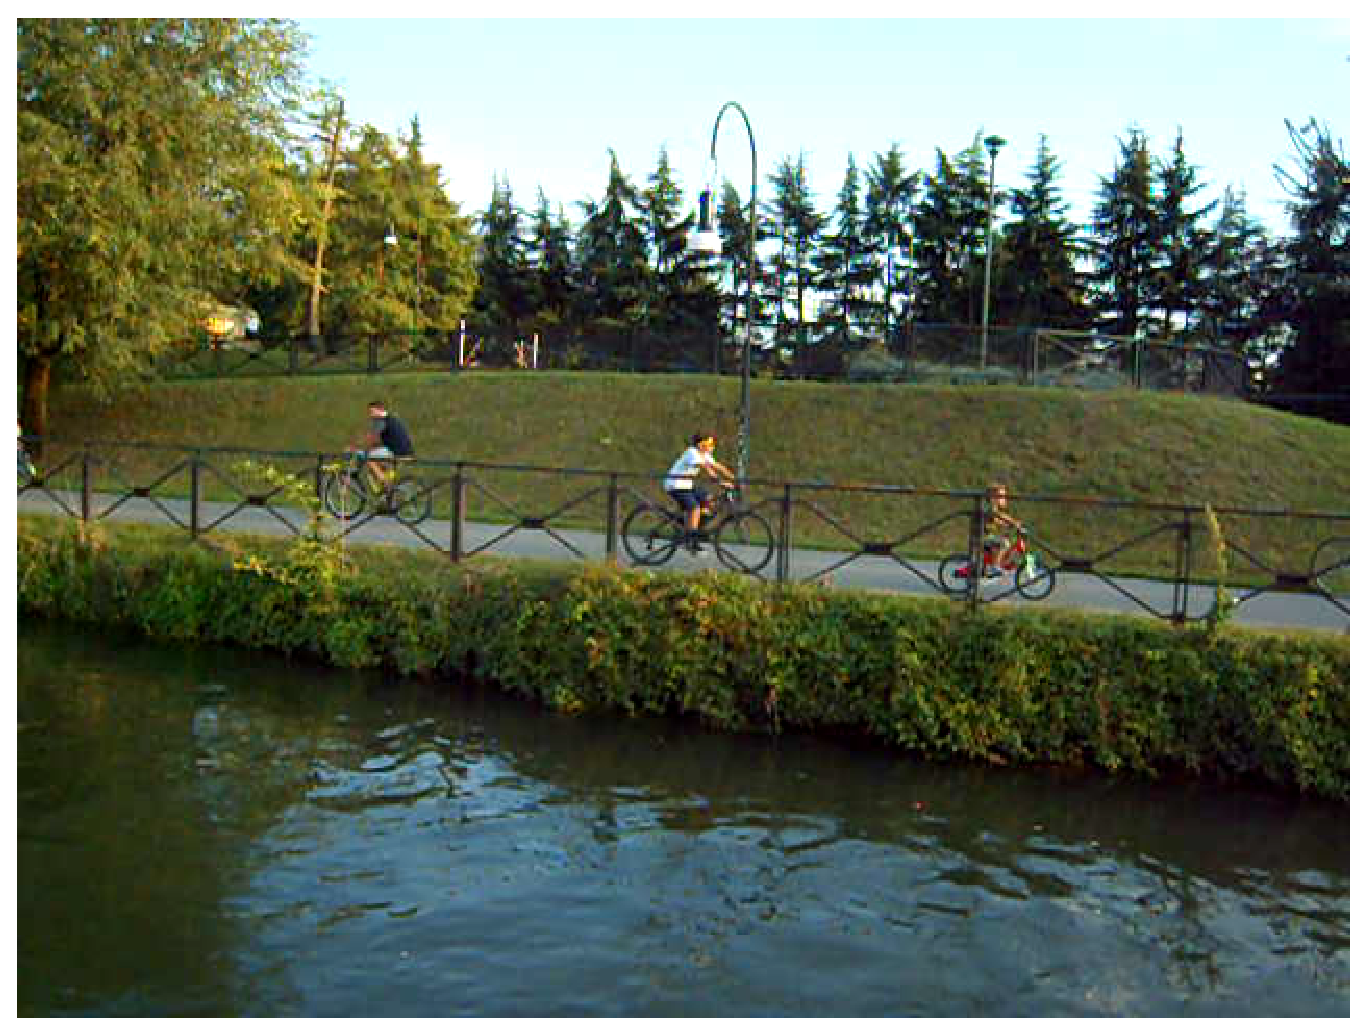
\includegraphics[width = 4cm]{./pictures/FPSalto/img0005}
	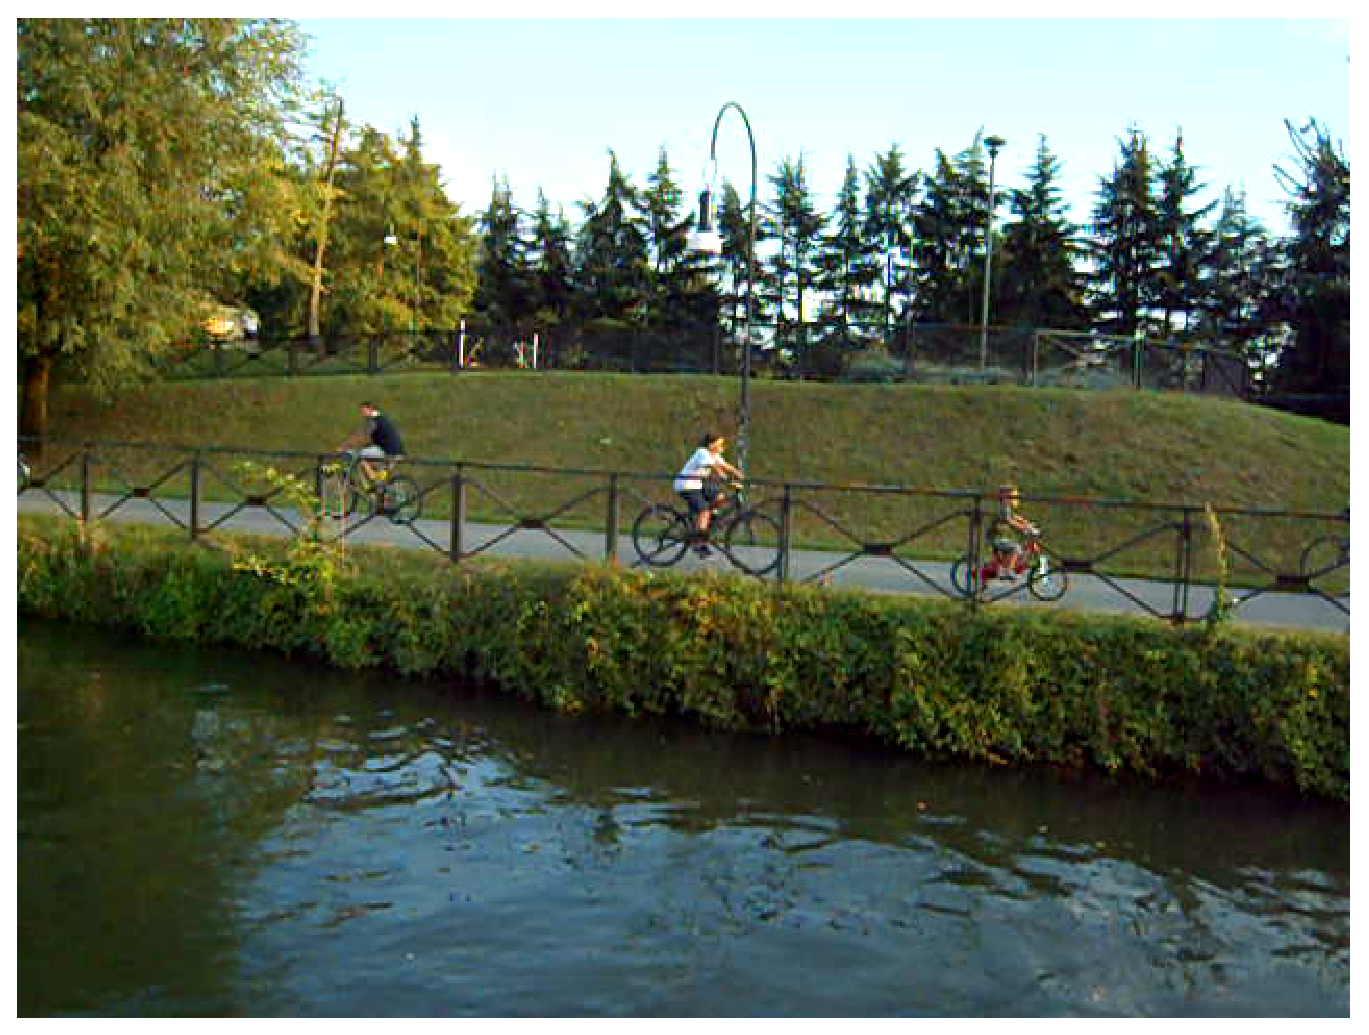
\includegraphics[width = 4cm]{./pictures/FPSalto/img0006}
	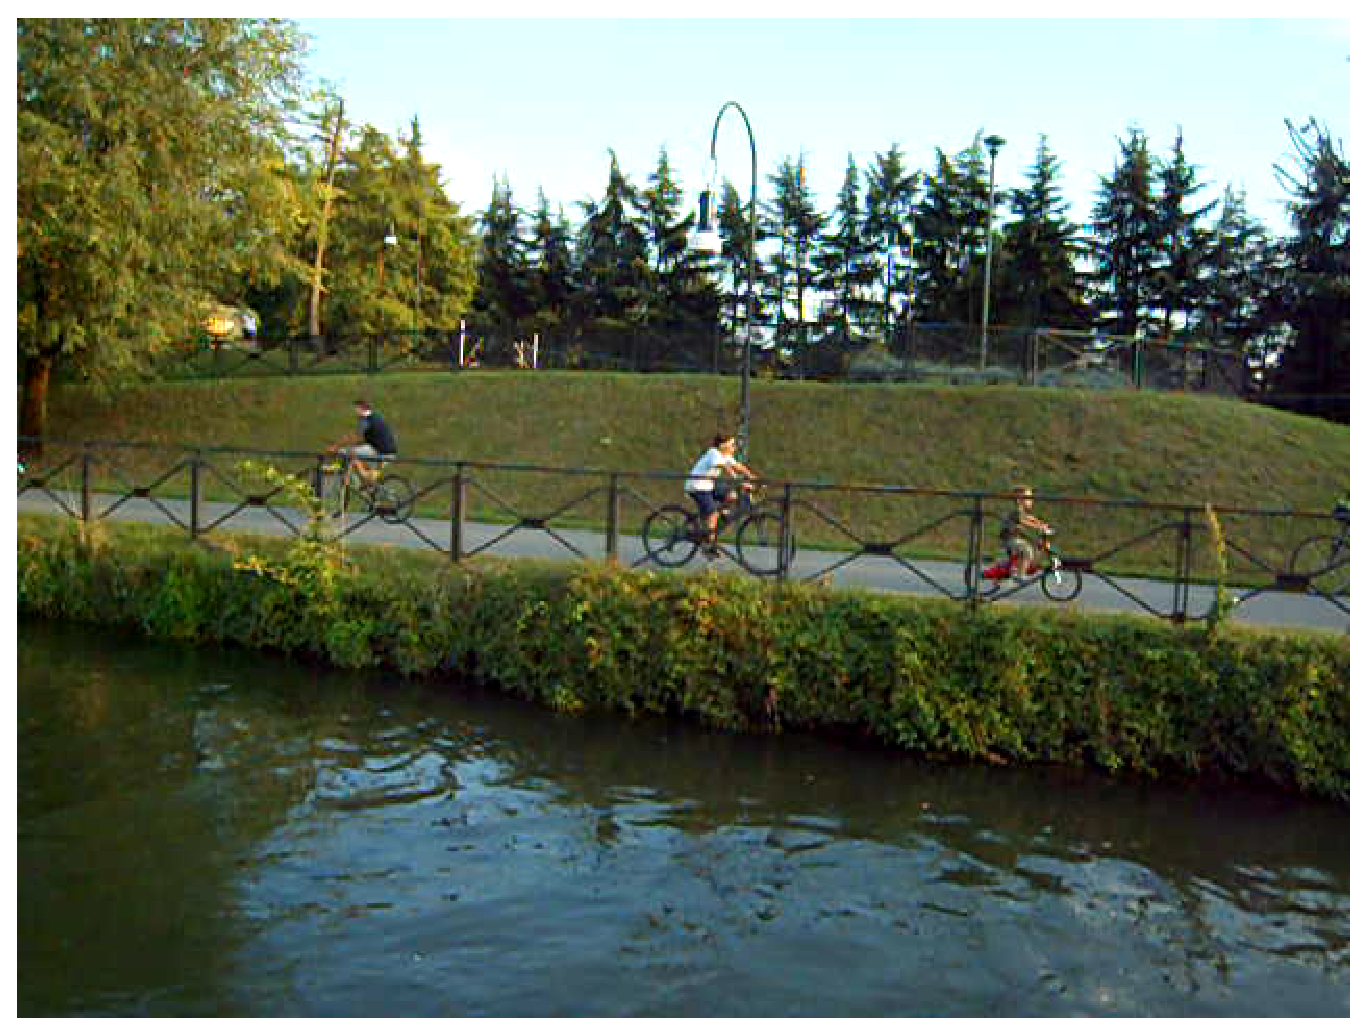
\includegraphics[width = 4cm]{./pictures/FPSalto/img0007}
	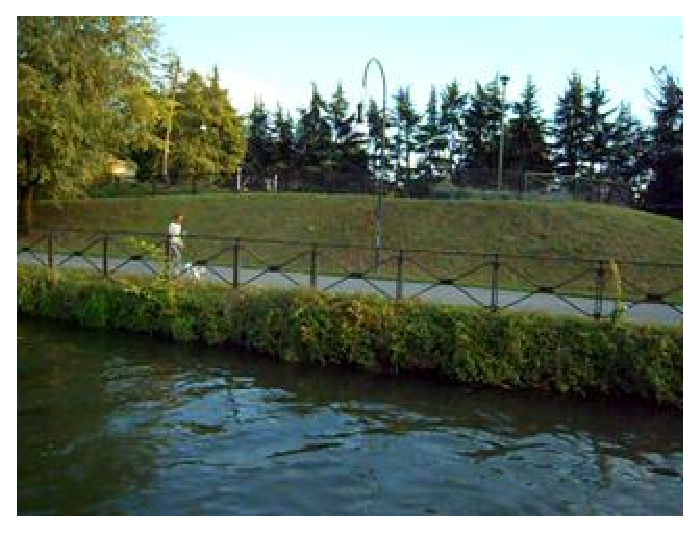
\includegraphics[width = 4cm]{./pictures/FPSalto/img0008}
	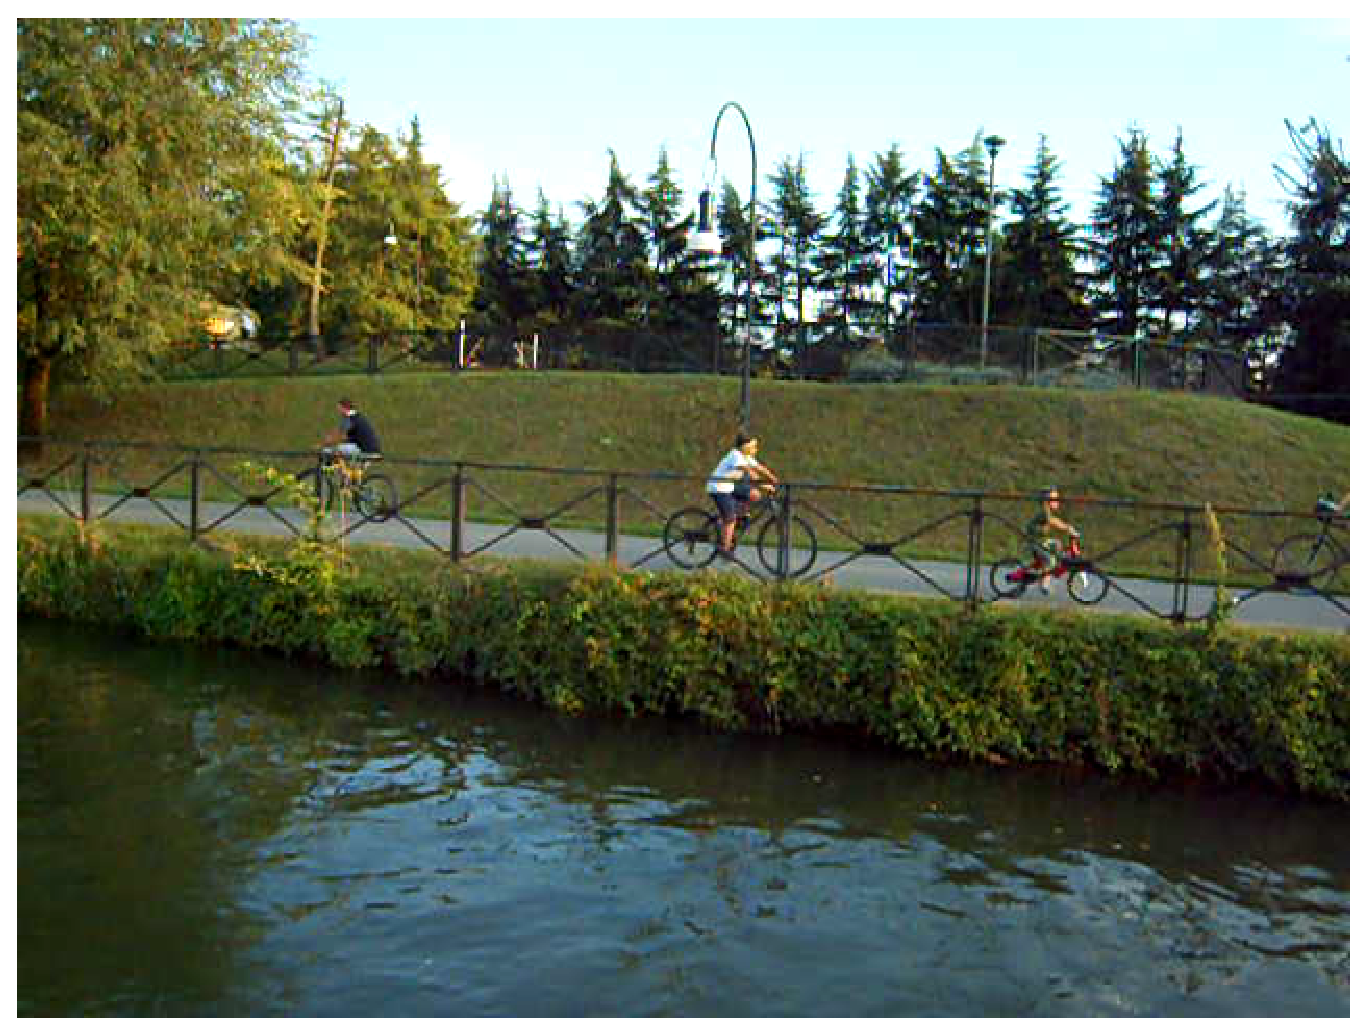
\includegraphics[width = 4cm]{./pictures/FPSalto/img0009}
	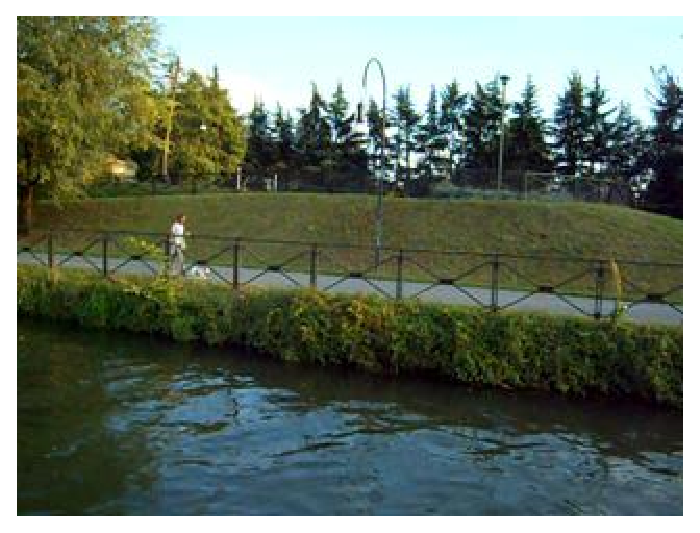
\includegraphics[width = 4cm]{./pictures/FPSalto/img0010}
	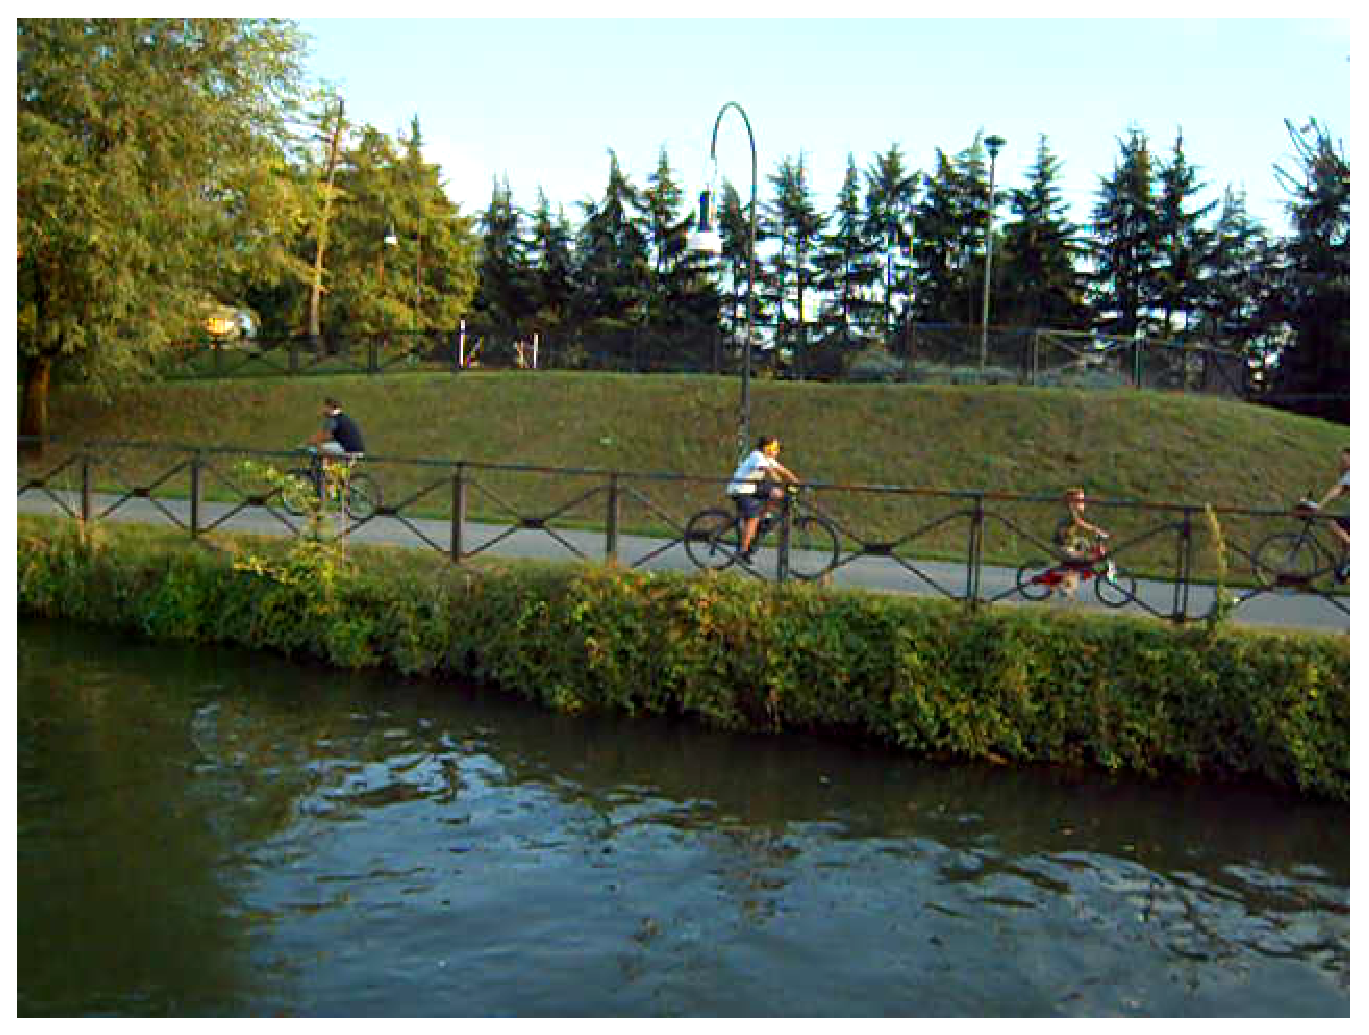
\includegraphics[width = 4cm]{./pictures/FPSalto/img0011}
	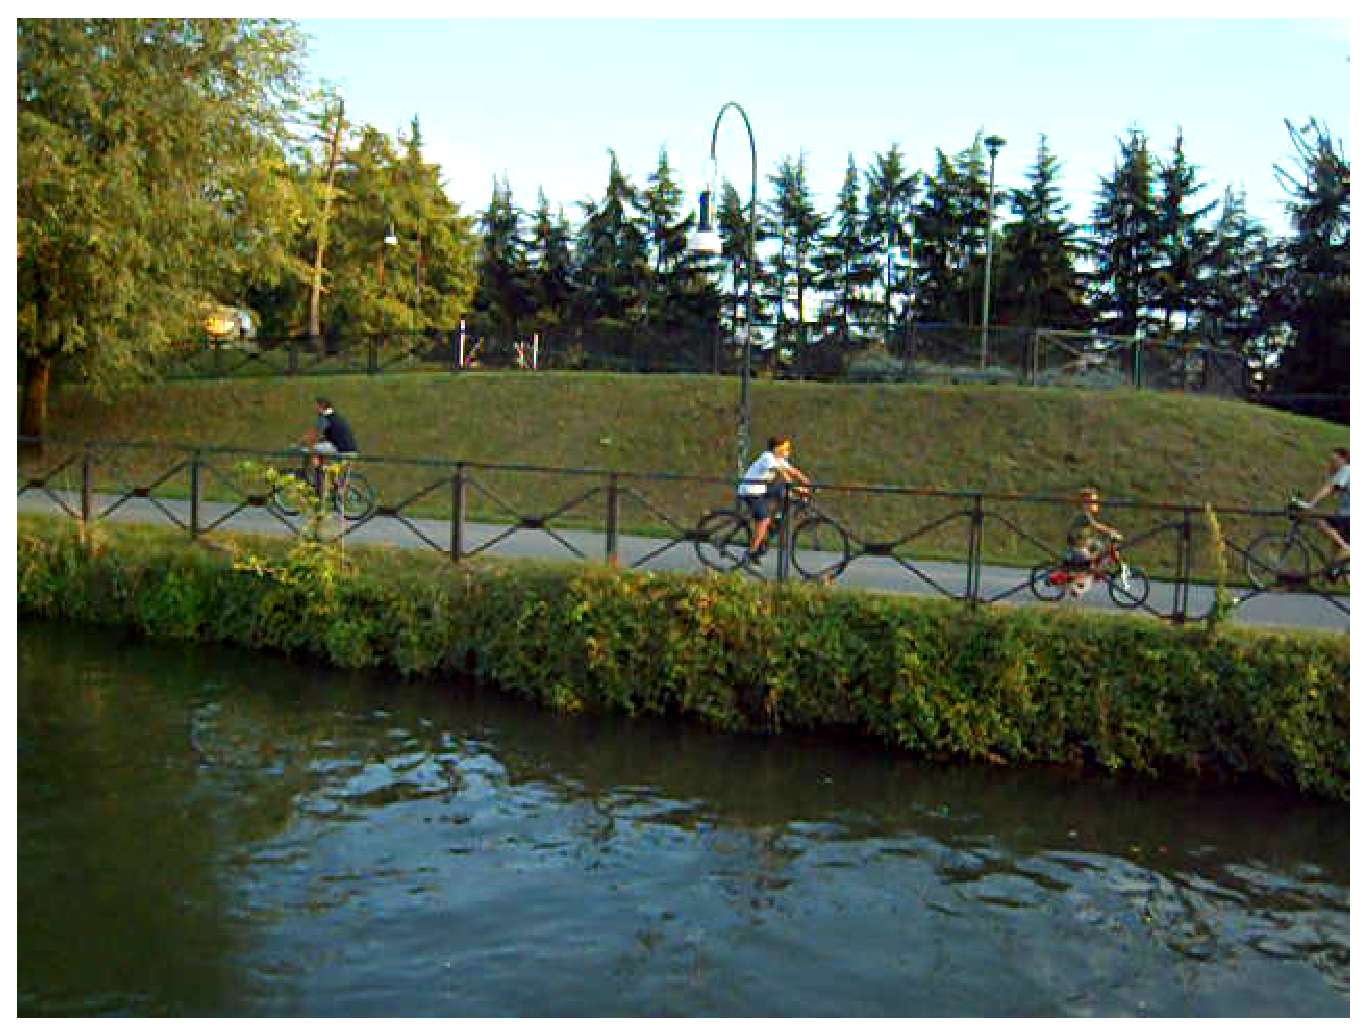
\includegraphics[width = 4cm]{./pictures/FPSalto/img0012}
	\caption{Sequenza di frame acquisiti a 30 fps}
	\label{fig:acquisizioneContinua}
\end{figure}
Un altro approccio consiste nell'analizzare la perdita di dettagli confrontando i contorni (\textit{edges}) del frame corrente con quelli del background.
Questo metodo, utilizzato in \cite{ellwart2012camera}, \cite{gil2007automatic}, \cite{harasse2004automated} e \cite{kryjak2012fpga}, consiste nell'estrarre i contorni dalle immagini secondo il metodo di Sobel \cite{sobel19683x3} o di Canny \cite{canny1986computational}, e confrontare il numero di pixel dei contorni con quelli del background. 
Quando il numero di pixel dei contorni del frame corrente $\sum edges(z_t)$ \`e $\Gamma$ volte pi\`u piccolo di quello del background $\sum edges(B_t)$:
\[ \sum edges(z_t) \leq \Gamma \sum edges(B_t), \]
dove $0<\Gamma<1$ \`e  un valore di soglia scelto in base alla sensibilit\`a che si vuole dare all'algoritmo.
\subsection{Tecniche basate su monitoraggio sequenziale}
Le tecniche viste finora, come \`e stato detto nel Paragrafo \ref{background}, permettono di aggiornare ciascun frame con un modello della scena che viene calcolato in base alle osservazioni precedenti.
\begin{figure}[tb]
	\centering
	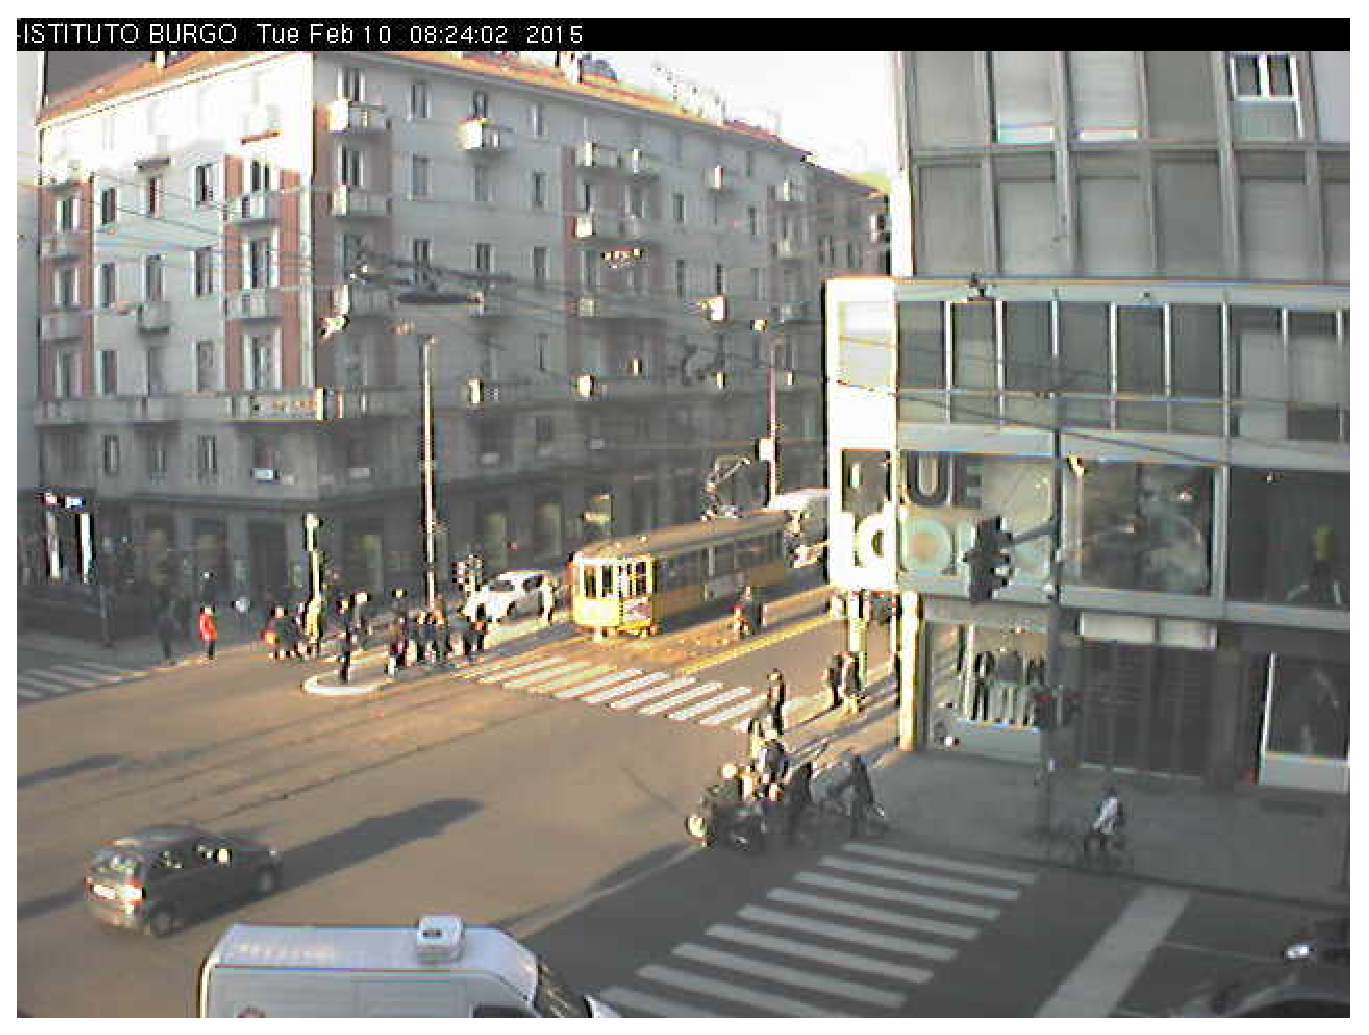
\includegraphics[width = 4cm]{./pictures/FPSbasso/image2691}
	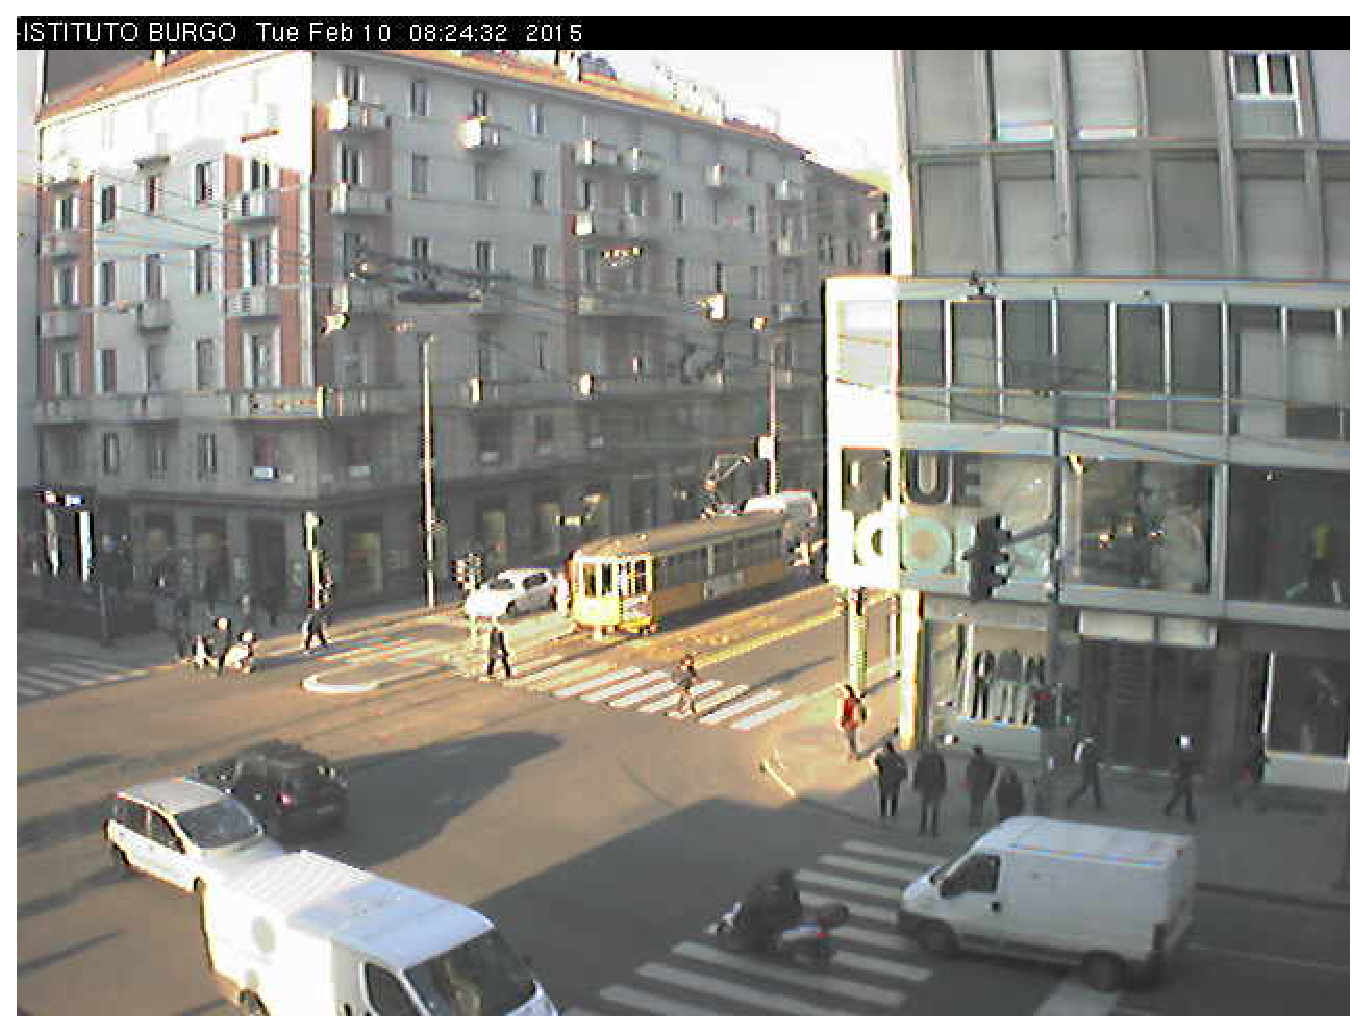
\includegraphics[width = 4cm]{./pictures/FPSbasso/image2692}
	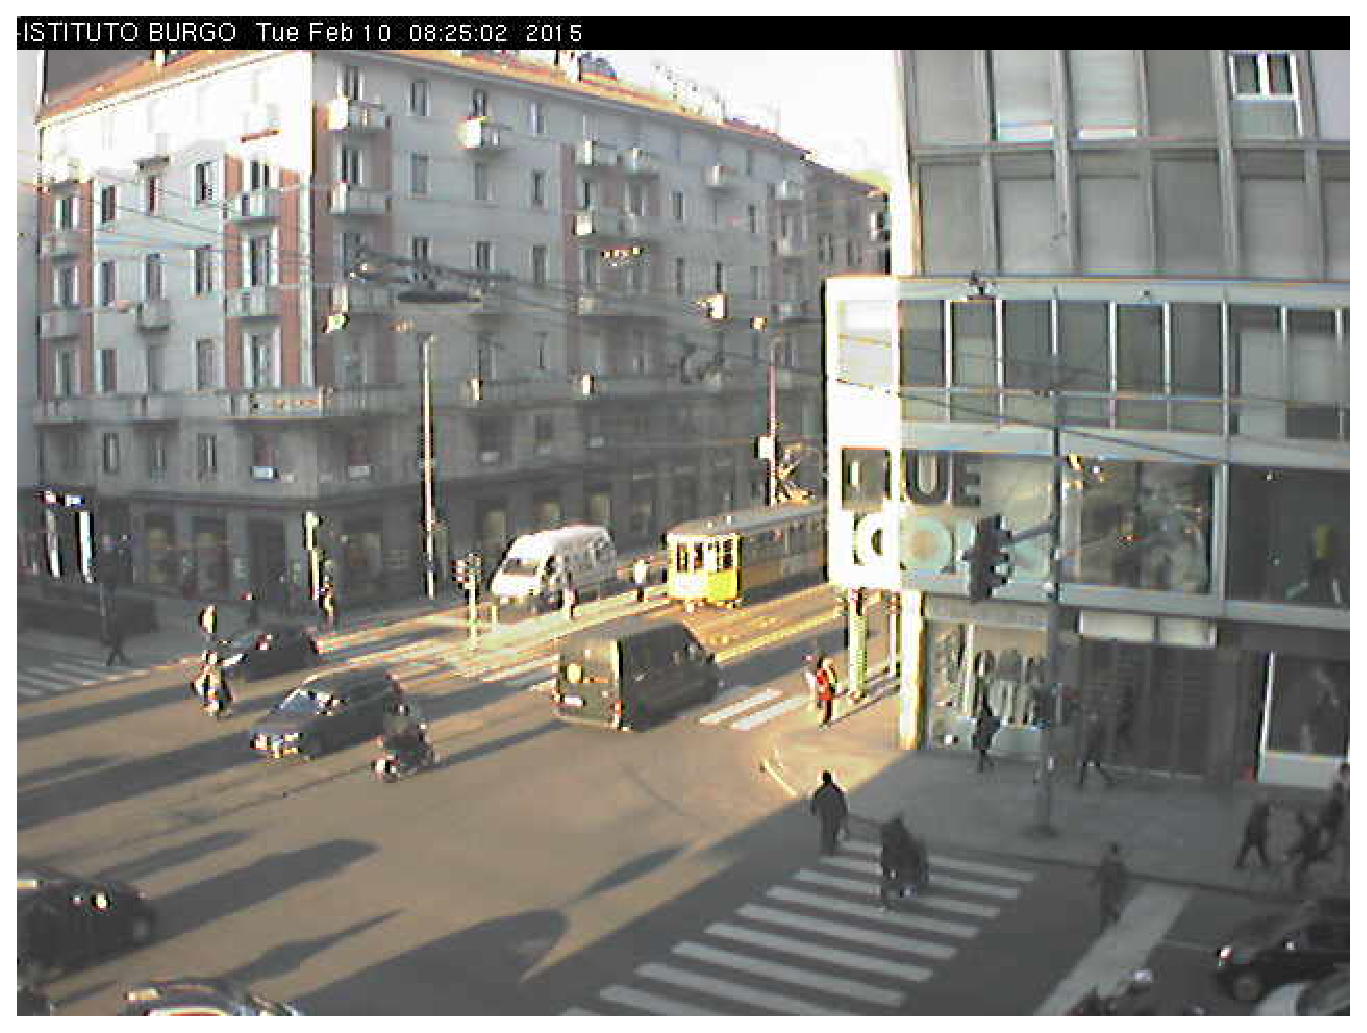
\includegraphics[width = 4cm]{./pictures/FPSbasso/image2693}
	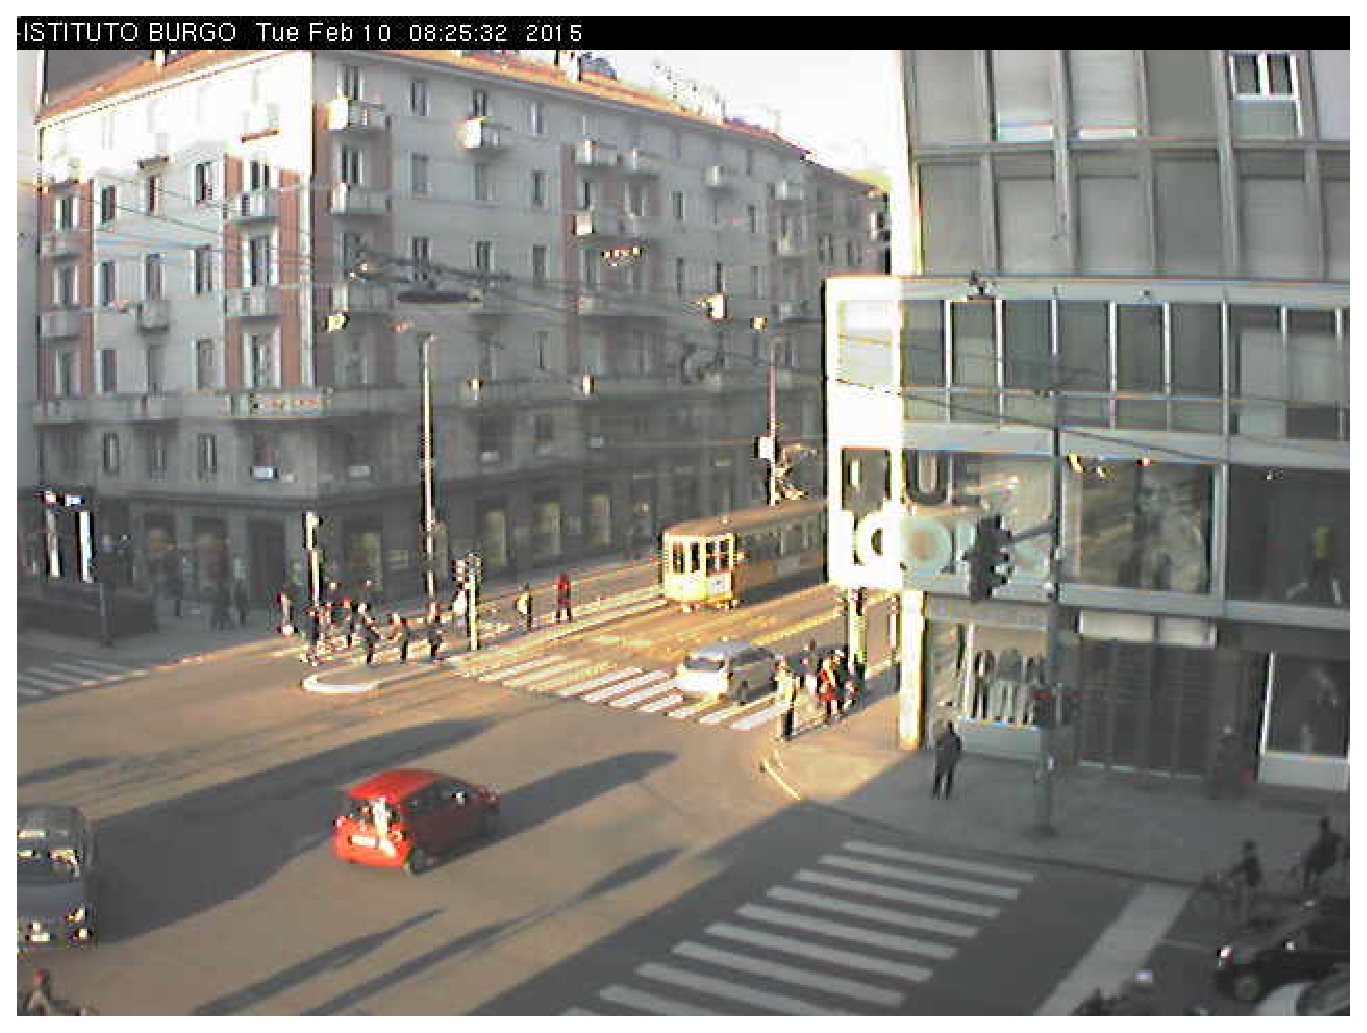
\includegraphics[width = 4cm]{./pictures/FPSbasso/image2694}
	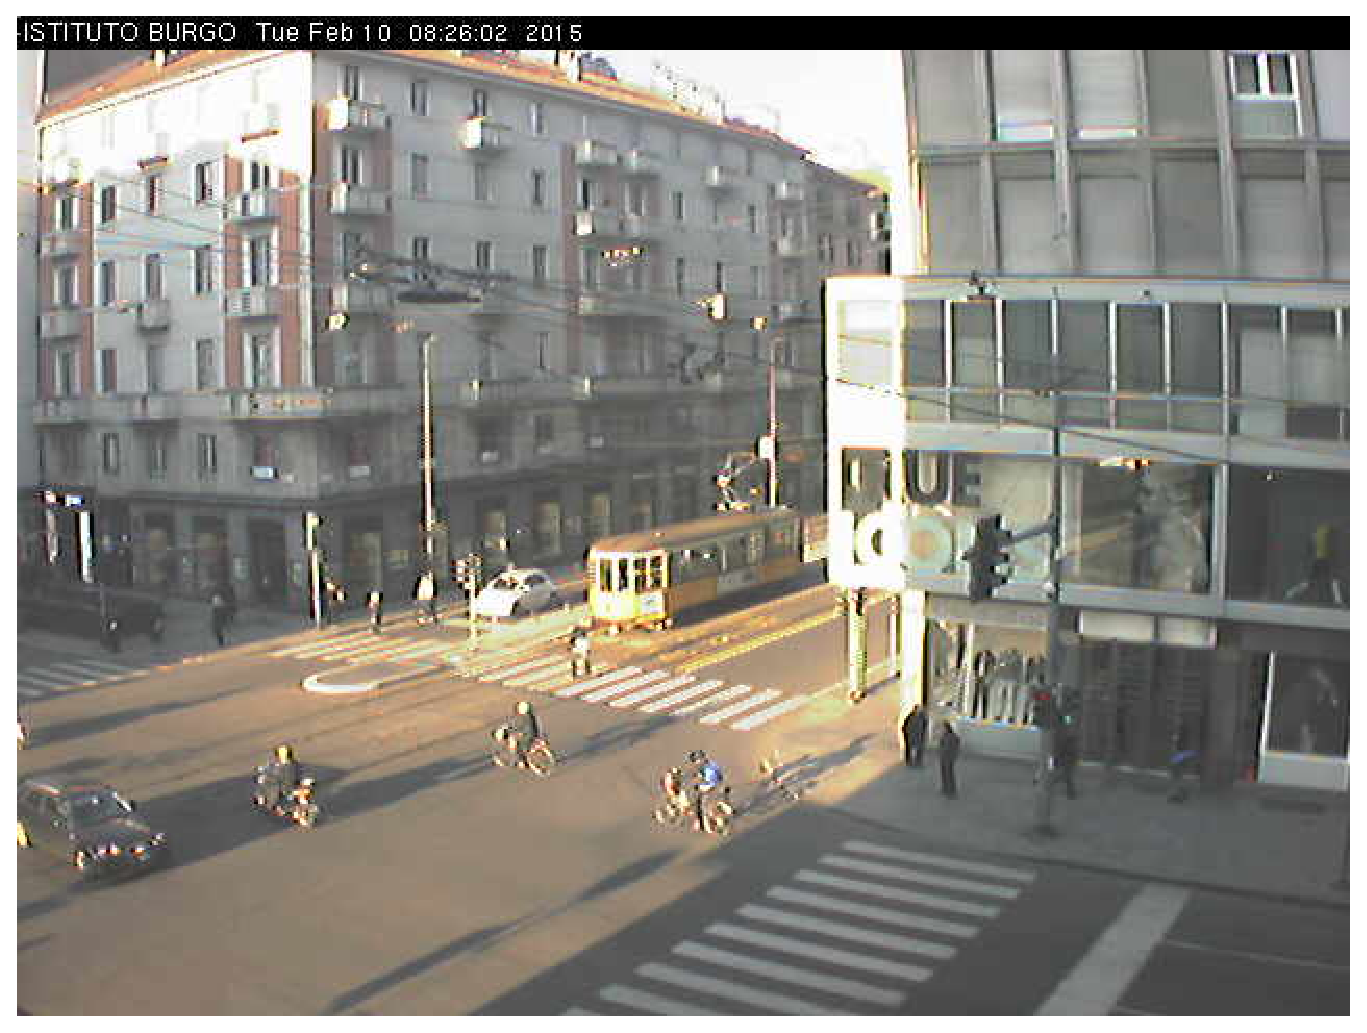
\includegraphics[width = 4cm]{./pictures/FPSbasso/image2695}
	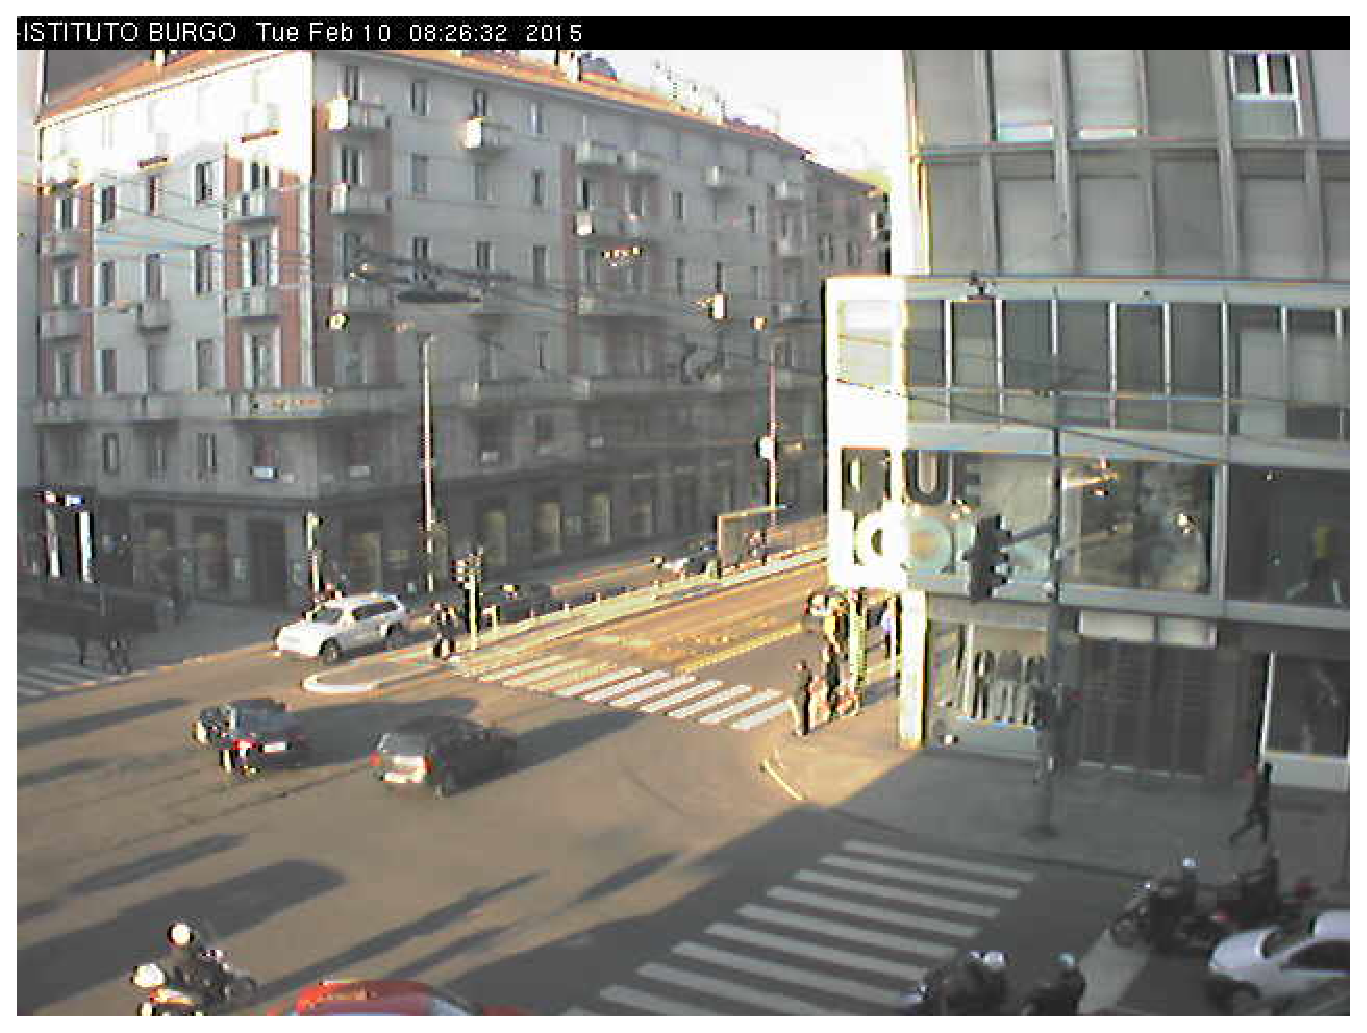
\includegraphics[width = 4cm]{./pictures/FPSbasso/image2696}
	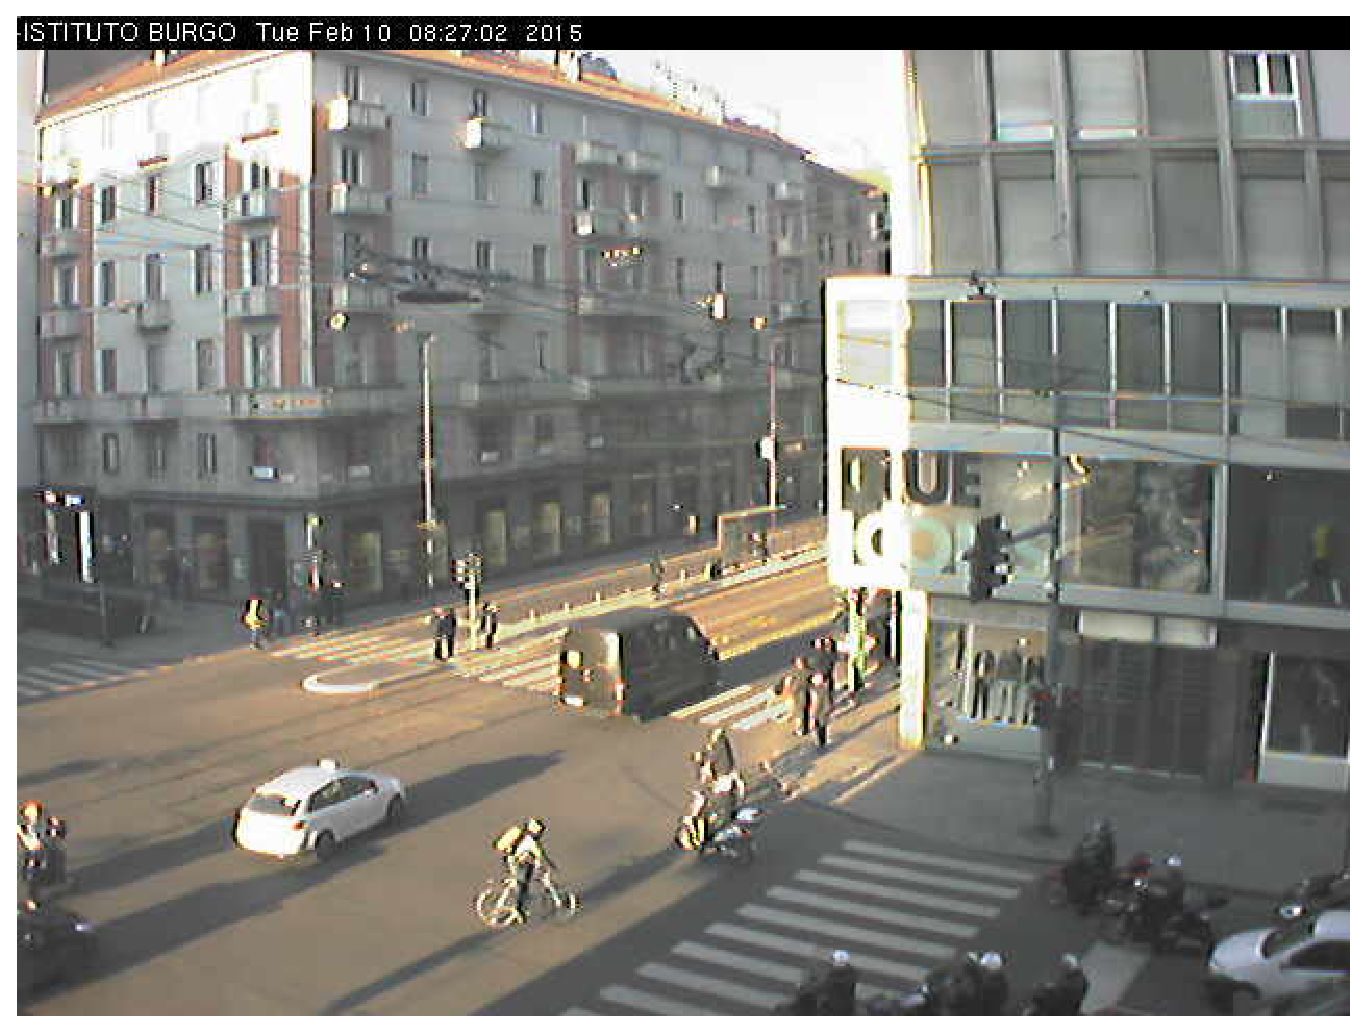
\includegraphics[width = 4cm]{./pictures/FPSbasso/image2697}
	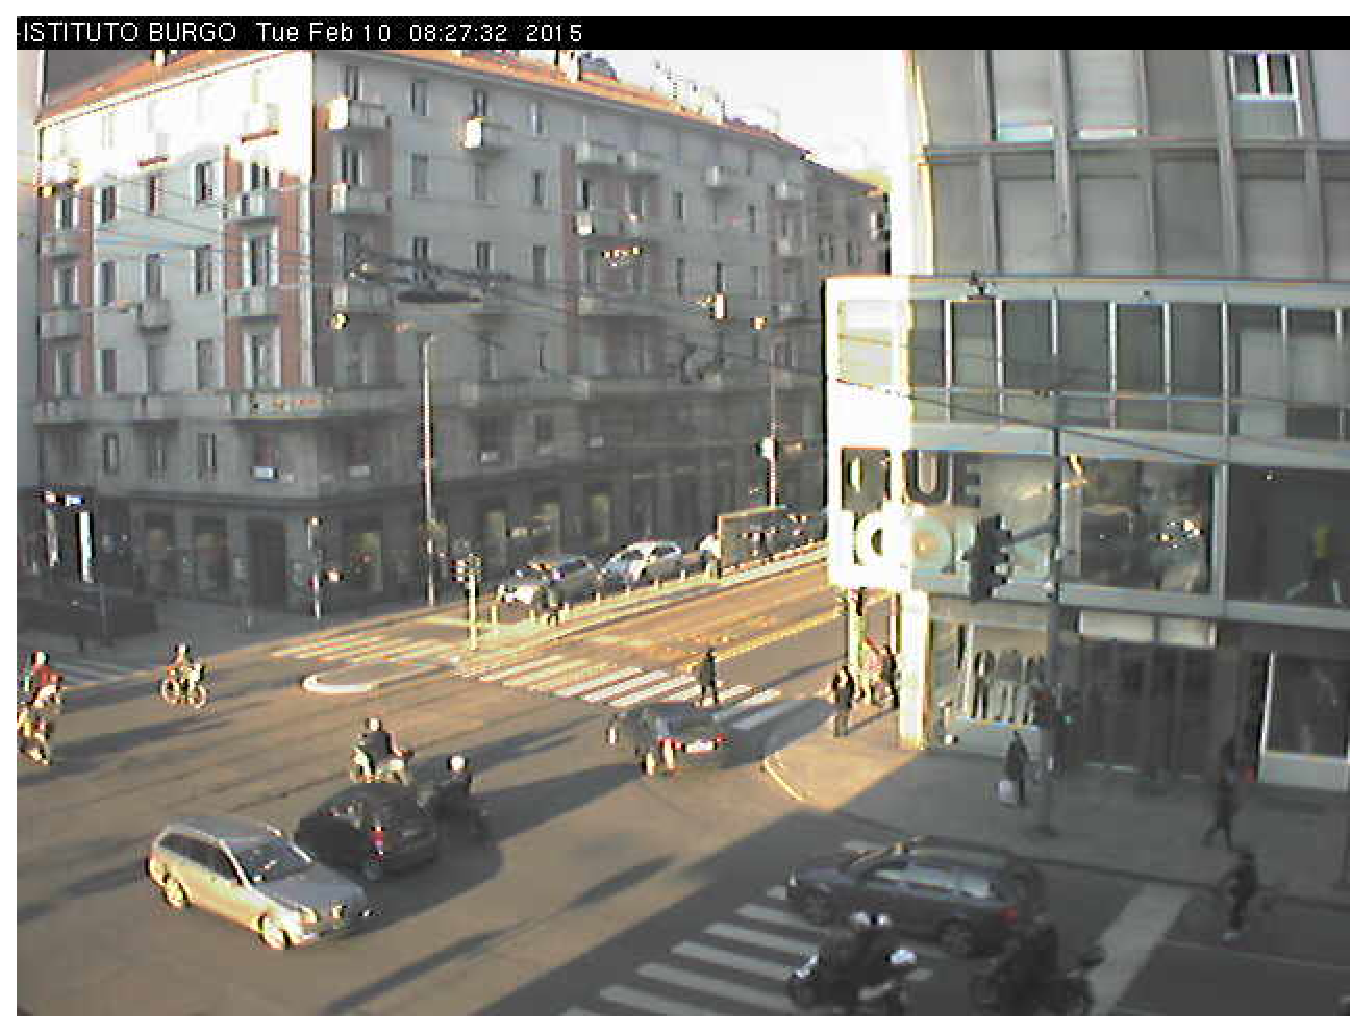
\includegraphics[width = 4cm]{./pictures/FPSbasso/image2698}
	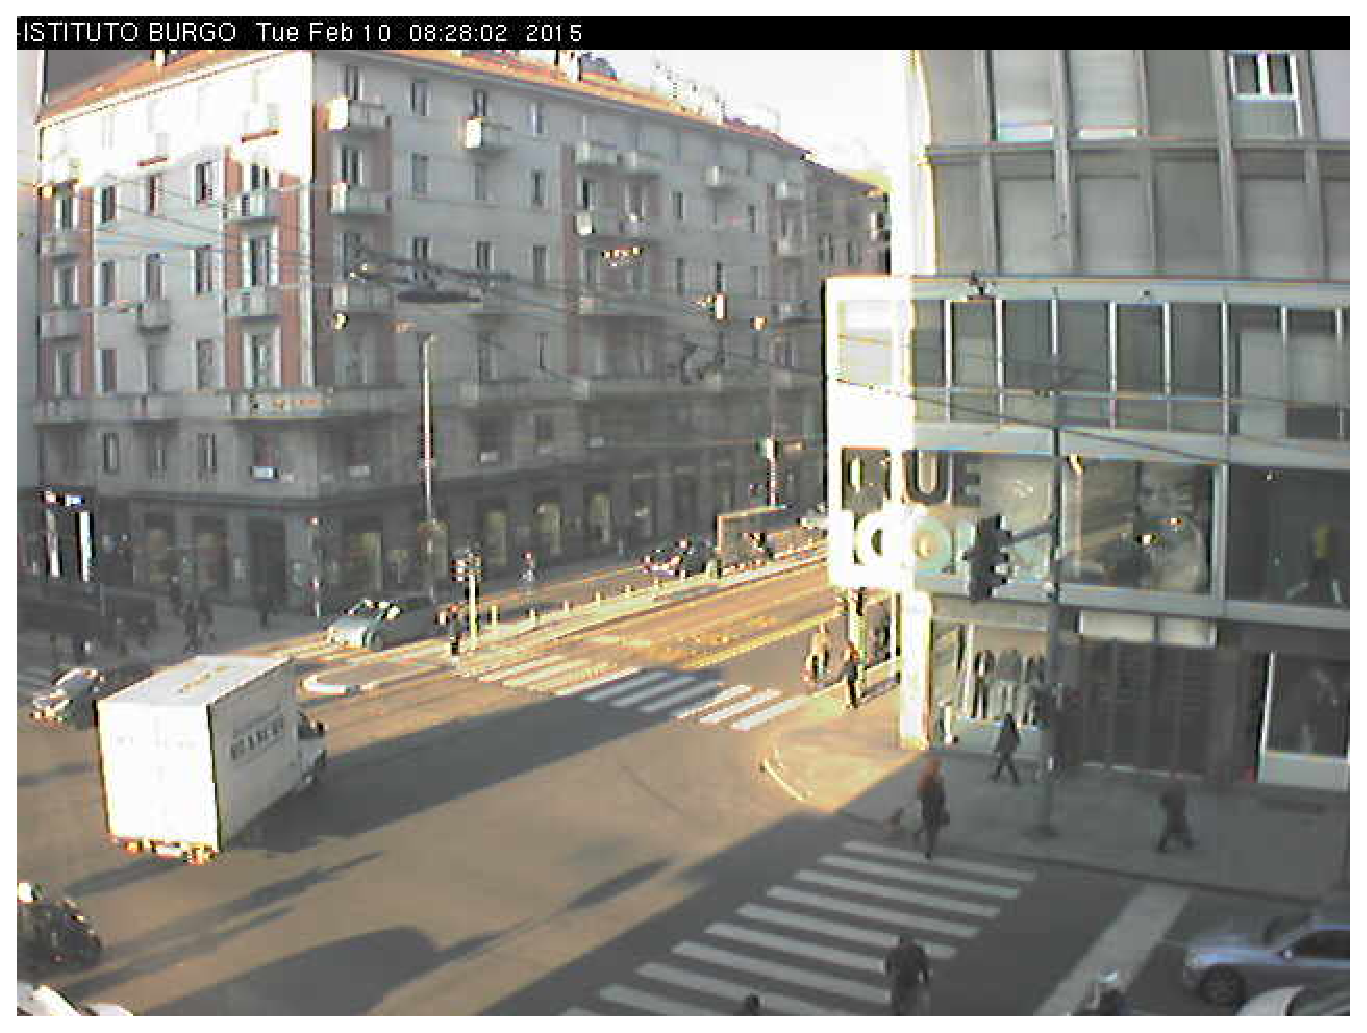
\includegraphics[width = 4cm]{./pictures/FPSbasso/image2699}
	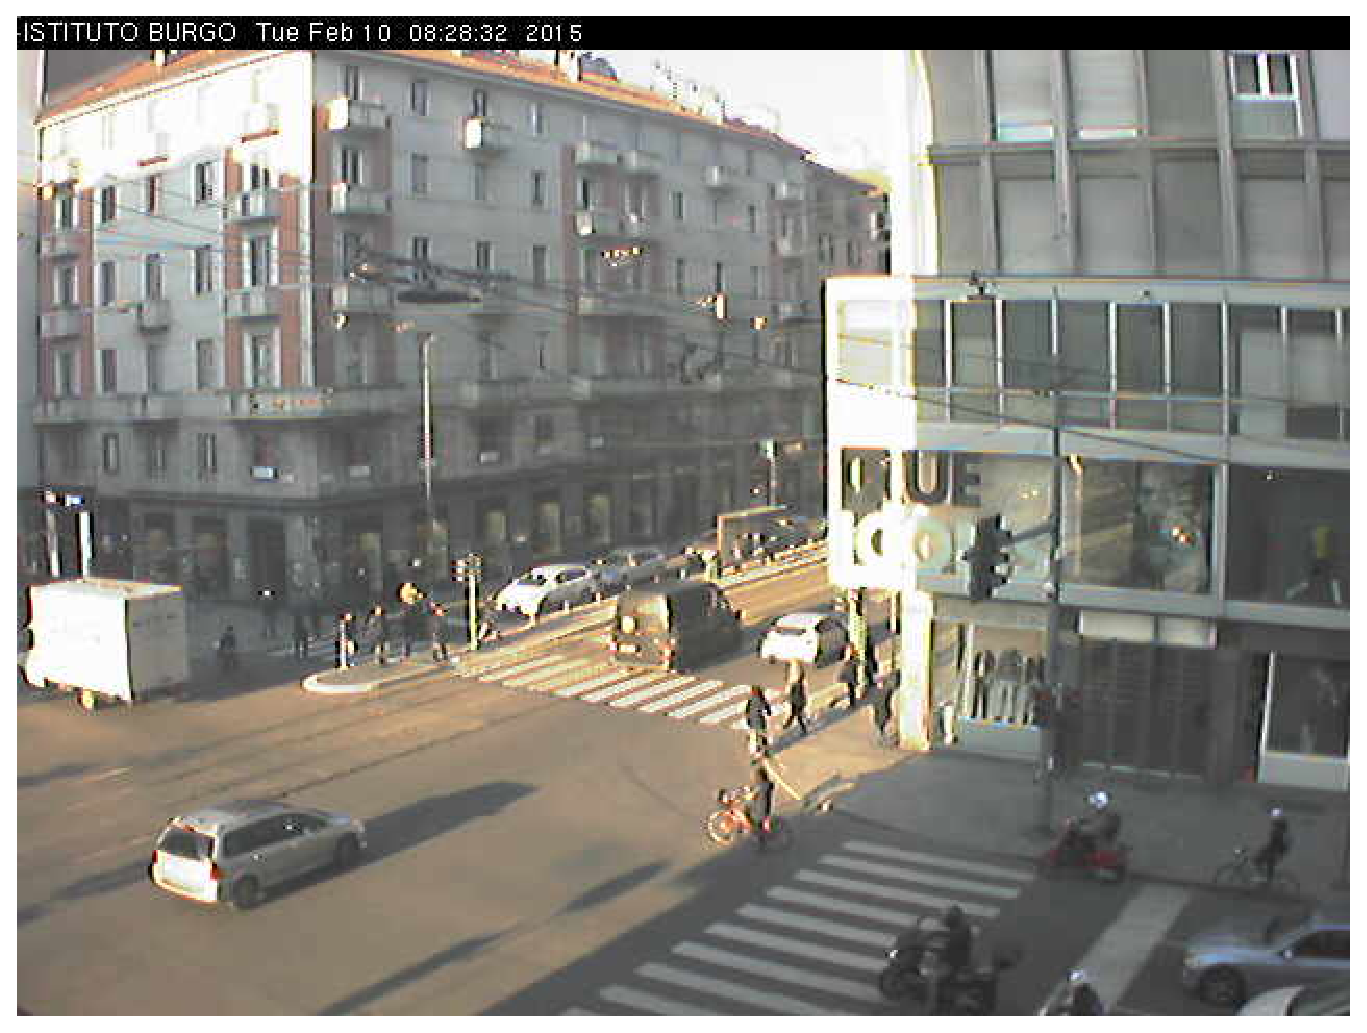
\includegraphics[width = 4cm]{./pictures/FPSbasso/image2700}
	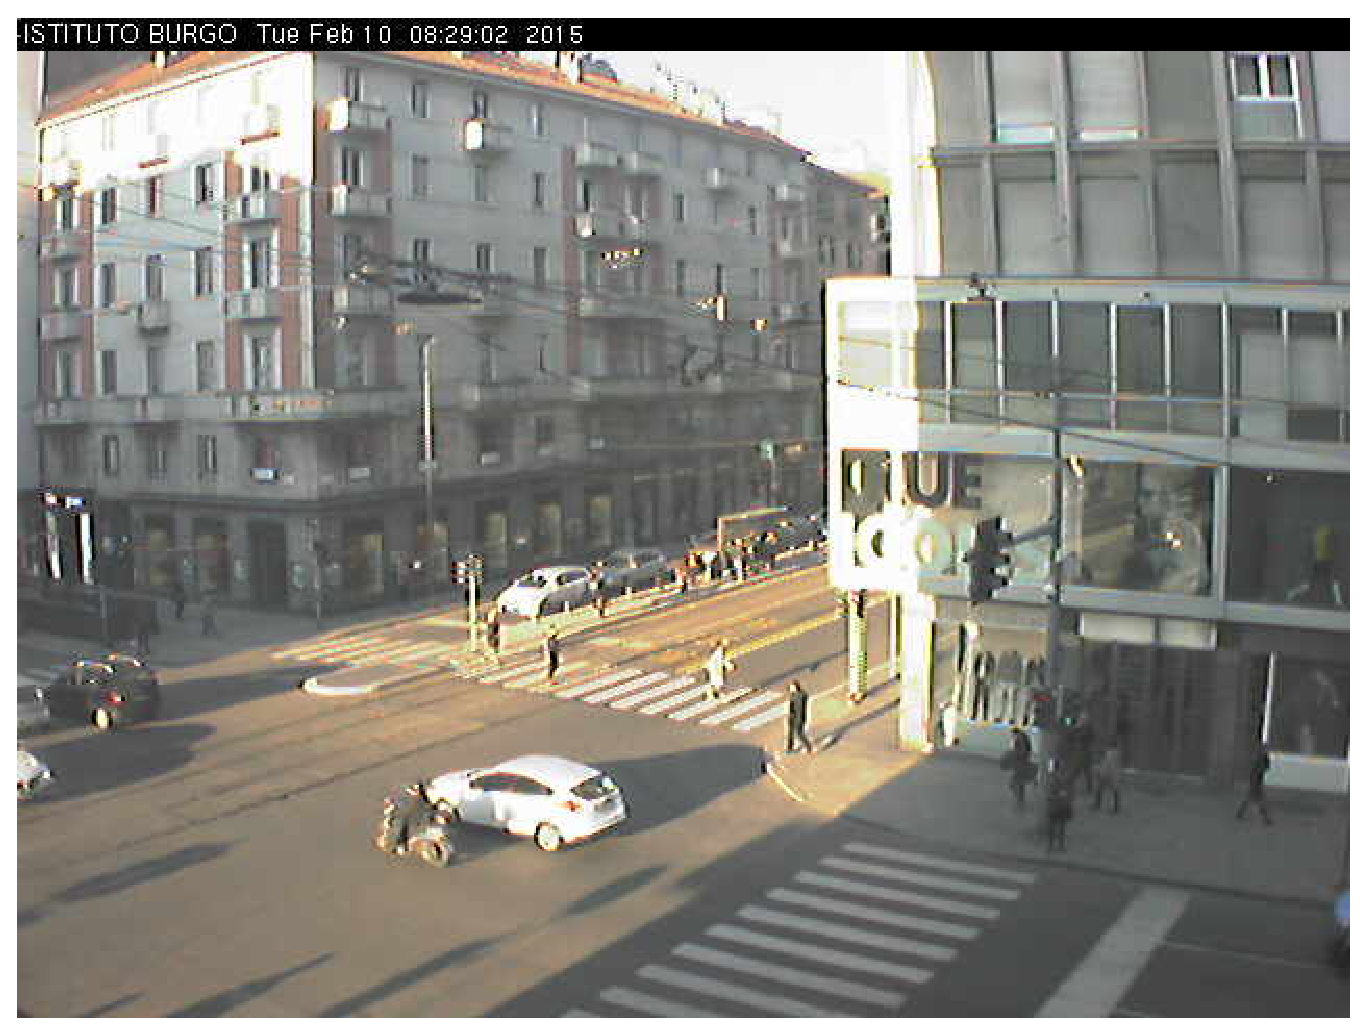
\includegraphics[width = 4cm]{./pictures/FPSbasso/image2701}
	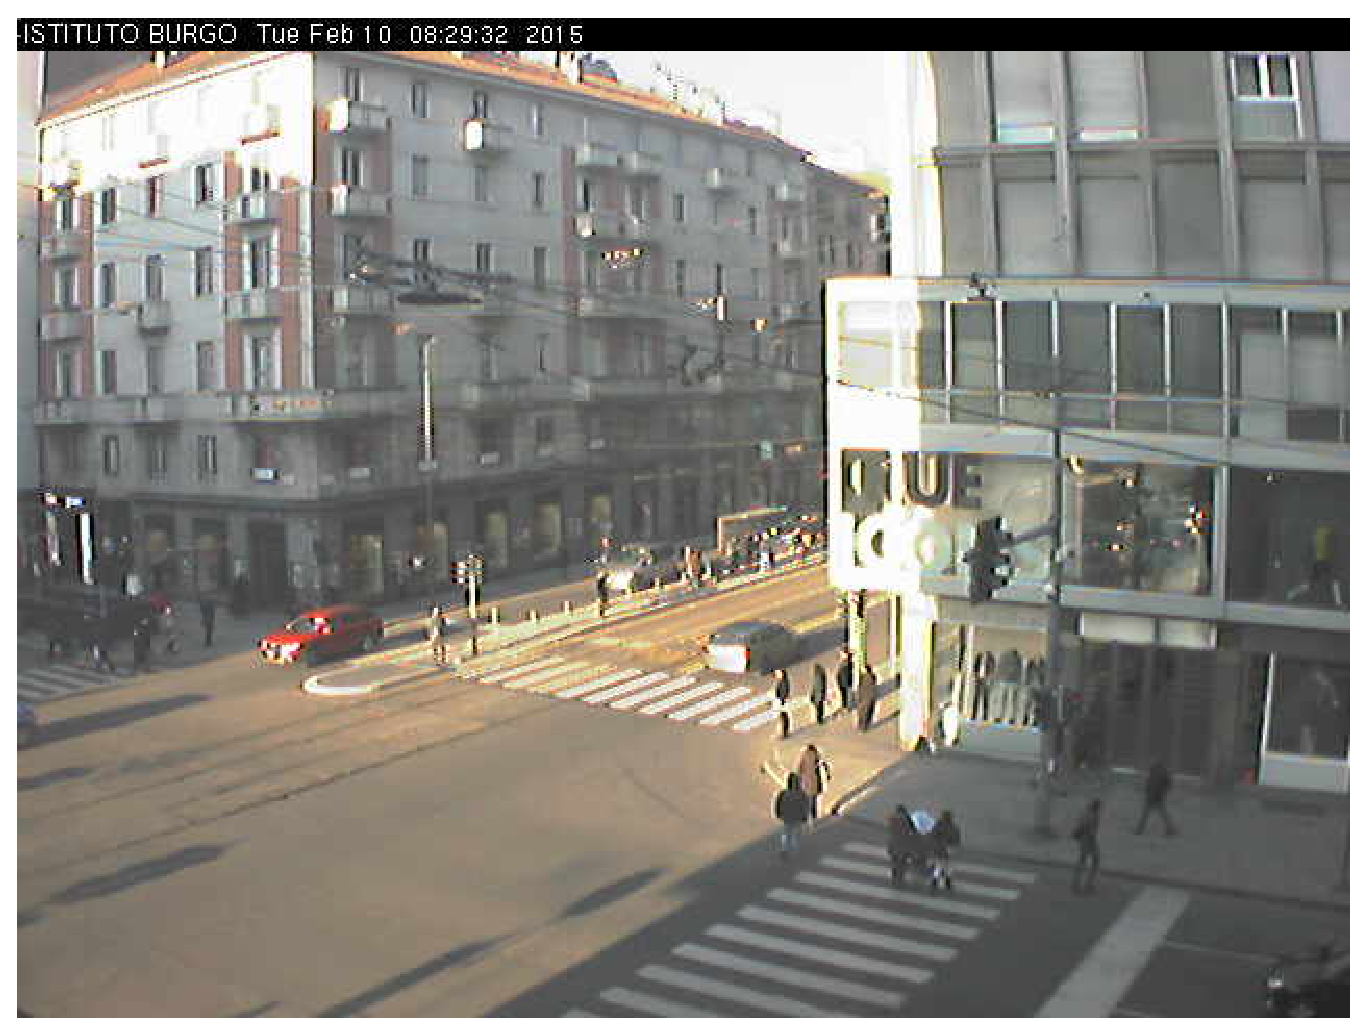
\includegraphics[width = 4cm]{./pictures/FPSbasso/image2702}
	\caption{Sequenza di frame acquisiti ogni 30 secondi}
	\label{fig:acquisizioneBassa}
\end{figure}
Questo approccio risulta fattibile nel caso in cui la camera operi con un framerate \textit{continuo}, solitamente tra i 30 frame per secondo (\textit{fps}) e i 2 fps. 
In questi casi, infatti, possiamo considerare che, tra un frame e il successivo, non avvengano grandi cambiamenti all'interno della scena e non cambi eccessivamente la luminosit\`a media.
La Figura \ref{fig:acquisizioneContinua} mostra come, in un'acquisizione fatta a 30 fps, le differenze tra frame consecutivi siano quasi inesistenti. 
Un evento di tampering pu\`o, quindi, essere identificato in maniera molto semplice, in quanto una differenza molto elevata tra il frame analizzato e il background pu\`o essere dovuto solamente a un evento di tampering sulla camera.
La Figura \ref{fig:acquisizioneBassa} mostra, invece, un esempio di frame acquisiti ogni 30 secondi.
Notiamo come le differenze tra immagini consecutive, in questo caso, siano pi\`u marcate rispetto al caso dell'acquisizione continua. 
Questo non permette l'impiego di un modello di background per il problema del tampering detection.
Evidenziamo, inoltre, che le tecniche viste finora richiedono che il sistema di monitoraggio possegga elevate capacit\`a computazionali, in quanto l'aggiornamento del background e l'analisi di tampering detection non pu\`o rallentare la frequenza di acquisizione.\\
Un approccio alternativo consiste nel monitorare nel tempo il comportamento di alcuni indicatori estratti dalle singole immagini acquisite.
Si presuppone che, quando il sistema di monitoraggio opera in condizioni di funzionamento \textit{ottimali}, gli indicatori analizzati presentino una certa \textit{stazionariet\`a}, ovvero siano considerati dei campioni \textit{indipendenti} tra loro e distribuiti secondo una stessa funzione di ripartizione.
L'evento di tampering viene considerato come un \textit{cambiamento nella stazionariet\`a} di questi indicatori.\\
Il monitoraggio pu\`o avvenire utilizzando tecniche statistiche, come ad esempio \textit{change-point method} (CPM) \cite{ross2011nonparametric} o \textit{change-detection test} \cite{pimentel2014review}.\\
Troviamo alcuni esempi nell'identificazione di sfocature: in \cite{tsesmelis2013tamper} la soluzione consiste nel monitorare nel tempo il \textit{numero di SURF} \cite{bay2006surf}, in quanto tali descrittori decrementano in maniera considerevole il loro numero in presenza di sfocature.
Notiamo, per\`o, che l'utilizzo di una tecnica del genere richiede un elevato numero di calcoli per ricavare le SURF.
Il metodo, quindi, si presta poco a essere utilizzato su sistemi di monitoraggio a basso consumo.\\
Un altro esempio \`e dato da \cite{alippi2010detecting}, dove le sfocature vengono identificate monitorando l'\textit{energia media del gradiente} delle immagini acquisite:
%\begin{equation}
%\label{eq:energyGradientSOA}
\[m_t = \mathcal{M}[z_t] = \int_{\mathcal{X}}\| \nabla z_t(x) \| _1 dx,\]
%\end{equation}  
dove $\| \cdot \|_1$ si riferisce alla \textit{norma} $\mathcal{L}_1$. 
Per identificare il cambio di stazionariet\`a di questo indicatore vengono utilizzate tecniche di CDT basate su \textit{somme cumulate} (CUSUM) \cite{alippi2008just}.\\
Il test statistico utilizzato non richiede alcuna informazione \textit{a priori} del processo che si sta monitorando, e sfrutta una sequenza iniziale $\{m_t\}, t=1,\dots,T$ di indicatori estratti da frame non sfocati, in modo da configurare automaticamente i suoi parametri. 
Tale sequenza prende il nome di \textit{training set} e, assumendo che i dati abbiano una distribuzione \textit{gaussiana,} permette di stimare i parametri di $m_t$ in assenza di sfocature che determinano l'\textit{ipotesi nulla} (indicata con $\Theta^0$), e di definire le \textit{ipotesi alternative}, indicate con $\Theta^1$, che identificano qualsiasi cambiamento non stazionario.\\
Per garantire una stima accurata dei parametri, \cite{alippi2010detecting} consiglia di utilizzare un training set ampio, ad esempio $T > 400$.
Il test opera su \textit{sotto-sequenze} di misure $m_t$ (ad esempio da $20$ misure) e stima la transizione da $\Theta^0$ a $\Theta^1$ misurando la \textit{log-verosimiglianza} tra la pdf in assenza di sfocature e le pdf delle varie ipotesi alternative nella sotto-sequenza $\tau$, ovvero
\[ r(\tau) = \ln \frac{N_{\Theta^1}(\phi_{\tau})}{N_{\Theta^0}(\phi_{\tau})}, \]
dove $\phi_{\tau}$ \`e il valore medio della misura $m_t$ nella sotto-sequenza $\tau$, e $N_{\Theta}$ \`e la \textit{distribuzione gaussiana multivariata} parametrizzata in $\Theta$.\\
Il metodo CUSUM considera la \textit{somma cumulata} 
\[ S(\tau) = \sum^\tau_{t=1} r(t) \]
e identifica un cambiamento in $m_t$ quando \[g(\tau)=S(\tau)-\nu(\tau),\] ovvero la differenza tra il valore della somma cumulata all'istante $\tau$ e il suo valore minimo nel tempo \[\nu(\tau)=\min_{t=1,...,\tau}S(t),\] supera una certa soglia $h$.\\
L'utilizzo di un descrittore leggero come l'energia media del gradiente permette di operare con una bassa complessit\`a computazionale, tanto da poter essere utilizzato come soluzione a livello di nodo per una \textit{wireless multimedia sensor network} (WMSN) \cite{akyildiz2007survey}.
D'altro canto, confrontato con le tecniche descritte nel Paragrafo \ref{background}, l'utilizzo di tecniche sequenziali genera un numero pi\`u alto di \textit{falsi allarmi}, il che si traduce, all'interno di una rete di sensori, in un aumento dei messaggi di allarme inviati, che devono essere considerati, quindi, come un costo.












